\documentclass[12pt,oneside]{book}

%%%%%%%%%%%%%%%%%%%%%%%%%%%%%%%%%%%%%%%%
% Include packages here
%%%%%%%%%%%%%%%%%%%%%%%%%%%%%%%%%%%%%%%%
\usepackage{amsmath}
\usepackage{amsfonts}
\usepackage{amssymb}
\usepackage{amsthm}
\usepackage{caption}
\usepackage{enumitem}
\usepackage[hyphens]{url}
\usepackage{hyperref}
\usepackage{listings}
\usepackage{graphics}
\usepackage{graphicx}
\usepackage{color}
\usepackage{subcaption}
\usepackage{todonotes}
%\usepackage{algorithm}
%\usepackage{algorithmic}
\usepackage{xspace}
\usepackage{tikz}
\usetikzlibrary{fit,positioning}

%%%%%%%%%%%%%%%%%%%%%%%%%%%%%%%%%%%%%%%
% Settings -- DO NOT CHANGE
%%%%%%%%%%%%%%%%%%%%%%%%%%%%%%%%%%%%%%%

\renewcommand{\baselinestretch}{1.3}
\hsize=5in
\vsize=7.5in
\hoffset=.25in
\voffset=.25in

\newcommand{\mychapter}[1]{\newpage \vspace*{0.01mm} \stepcounter{chapter}
    \begin{center}
    {\huge \bf Chapter \space  \thechapter \vspace*{1em}  \par
        #1\baselineskip=1.0\normalbaselineskip\par}
         \end{center}
            \vspace*{3ex} \par
\addcontentsline{toc}{chapter}{\protect \numberline{\thechapter}{#1}}}

\newcommand{\myappendix}{\newpage \vspace*{0.01mm} \stepcounter{chapter}
        \begin{center}
        {\LARGE \bf Appendix \space   \par
                \baselineskip=1.0\normalbaselineskip\par}
                 \end{center}
                        \vspace*{3ex} \par
\addcontentsline{toc}{chapter}{Appendix}}

\newcommand{\eg}{\emph{e.g.,}\@\xspace}
\newcommand{\ie}{\emph{i.e.,}\@\xspace}
\newcommand\clarQ{\textsc{clarQ}\@\xspace}

\makeatletter
\newcommand{\etc}{%
    \@ifnextchar{.}%
        {\emph{etc}}%
        {\emph{etc.}\@\xspace}%
}
\newcommand{\etal}{%
    \@ifnextchar{.}%
        {\emph{et al}}%
        {\emph{et al.}\@\xspace}%
}
\makeatother


\newcommand{\vect}[1]{\boldsymbol{#1}}
\newcommand{\argmax}[1]{\underset{#1}{arg\,max}\,\,}
\newcommand{\argmin}[1]{\underset{#1}{arg\,min}\,\,}
\newcommand{\expect}[1]{\langle #1 \rangle}
\newcommand{\normone}[1]{\| #1 \|_1}
\newcommand{\meanvar}[2]{#1\,{\scriptsize (#2)}}
\newcommand{\bigspace}[0]{\;\;\;\;\;\;\;\;\;\;\;\;\;\;\;\;\;\;\;\;\;\;\;\;\;\;\;\;\;\;\;\;\;\;\;\;\,}
\newcommand{\naive}{na\"ive }
\newcommand{\refeq}[1]{Eq.~(\ref{#1})}
\newcommand{\reffig}[1]{Figure \ref{#1}}
\newcommand{\what}[1]{\widehat{#1}}

% This fixes the page numbering in the bibliography
\makeatletter
\let\ps@plain\ps@myheadings
\makeatother

%%%%%%%%%%%%%%%%%%%%%%%%%%%%%%%%%%%%%%%%%%%%%%%%%
% Definitions of new theorem environments
%%%%%%%%%%%%%%%%%%%%%%%%%%%%%%%%%%%%%%%%%%%%%%%%%
\newtheorem{theorem}{Theorem}[chapter]
%% To number theorems, etc., in the same sequence as equations, use this instead:
%%    \newtheorem{theorem}[equation]{Theorem}
%% and replace [theorem] with [equation] in each of the following commands. 
\newtheorem{definition}[theorem]{Definition}
\newtheorem{proposition}[theorem]{Proposition}
\newtheorem{fact}[theorem]{Fact}
\newtheorem{corollary}[theorem]{Corollary}
\newtheorem{lemma}[theorem]{Lemma}
\newtheorem{state}[theorem]{Statement}
\newtheorem{claim}[theorem]{Claim}
\newtheorem{example}[theorem]{Example}
\newtheorem{problem}[theorem]{Problem}
\newtheorem{question}[theorem]{Question}
\newtheorem{conjecture}[theorem]{Conjecture}

\setlength{\parindent}{0.3cm}
\setlength{\headsep}{1.15in}
\setlength{\topmargin}{-.5in}

%%%%%%%%%%%%%%%%%%%%%%%%%%%%%%%%%%%%%%%
% Let's go !
%%%%%%%%%%%%%%%%%%%%%%%%%%%%%%%%%%%%%%%



\begin{document}
\clearpage
\pagestyle{empty}
%%%%%%%%%%%%%%%%%%%%%%%%%%%%%%%%%%%%%%%%%%%%%%%%%
% Comment/uncomment the list you wish to include
%%%%%%%%%%%%%%%%%%%%%%%%%%%%%%%%%%%%%%%%%%%%%%%%%
% this prevents page numbers on table of contents pages
% if there's more than one of them
\addtocontents{toc}{\protect\thispagestyle{empty}}

\tableofcontents  \thispagestyle{empty}
\listoffigures    \thispagestyle{empty}
\listoftables     \thispagestyle{empty}
%\listofalgorithms \thispagestyle{empty}


%%%%%%%%%%%%%%%%%%%%%%%%%%%%%%%%%%%%%%%%%%%%%%%%%
% Define other commands here
%%%%%%%%%%%%%%%%%%%%%%%%%%%%%%%%%%%%%%%%%%%%%%%%%
\newcommand{\Rset}{\ensuremath{\mathbb{R}}}
\newcommand{\Nset}{\ensuremath{\mathbb{N}}}
\newcommand{\Qset}{\ensuremath{\mathbb{Q}}}
\newcommand{\Zset}{\ensuremath{\mathbb{Z}}}


%%%%%%%%%%%%%%%%%%%%%%%%%%%%%%%%%%%%%%%%%%%%%%%%%
% Include your .tex sources here
%%%%%%%%%%%%%%%%%%%%%%%%%%%%%%%%%%%%%%%%%%%%%%%%%
\pagestyle{myheadings}
\chapter{Introduction}
\setcounter{page}{1}

It has long been a dream to communicate with a computer as one might with another human being using natural language.
We are now closer to this dream, as natural language interfaces become increasingly popular.
Our phones are already reasonably good at recognizing speech, and personal assistants, such as Apple Siri, Google Assistant, Microsoft Cortana, Amazon Alexa, \etc, help us with everyday tasks and answer some of our questions.
Chat bots are arguably considered ``the next big thing'', and a number of startups developing this kind of technology have emerged in Silicon Valley and around the world\footnote{\href{url}{http://time.com/4194063/chatbots-facebook-messenger-kik-wechat/}}.

Question answering is one of the major components of such personal assistants.
Existing techniques already allow users to get direct answers to some of their questions.
However, by some estimates\footnote{\href{url}{https://www.stonetemple.com/the-growth-of-rich-answers-in-googles-search-results/}} for $\sim 70\%$ of more complex questions users still have to dig into the ``10 blue links'' from search engine results page and extract or synthesize answers from information buried within the retrieved documents.
In order to make a shift towards more intelligent personal assistants, this gap needs to be closed.
Therefore, in my dissertation, I focus on helping users solve their informational needs by improving question answering methods and techniques.

User questions vary in many different aspects, and each type has its own set of challenges~\cite{voorhees2001trec,yang2016beyond}.
It is common to divide questions into \textit{factoid} and \textit{non-factoid}.
Factoid questions are inquiring about certain facts and can be answered with entity names or attributes, such as dates or numbers.
An example of a factoid question is ``\textit{What book did John Steinbeck wrote about the people in the dust bowl?}'' (answer: ``\textit{The Grapes of Wrath}'').
Of course, there is a variety of questions, that do not fall into this category, \eg how-to, ``why'' questions, recommendation and opinion questions, \etc
The literature usually refers to all such questions as ``\textit{non-factoid}''.
An example of such question is ``\textit{Why did John Steinbeck name his book the Grapes of Wrath?}''.
Most of the research in automatic question answering focused on factoid questions \cite{BerantCFL13:sempre,Cafarella:2008:WEP:1453856.1453916,voorhees2001trec,lin2007exploration}, but relatively recently more and more works have started targeting the category of non-factoid questions~\cite{overviewliveqa15,cohen2016end,fried2015higher,surdeanu2011learning,sharp2015spinning,tymoshenko2016learning,yang2016beyond}.

\begin{table}[h!t]
	\centering
	\small
	\begin{tabular}{p{2cm}|p{5.3cm}|p{5.3cm}}
		& Unstructured data & Structured data \\
		\hline
		Factoid questions & \multicolumn{1}{|c|}{Text} & \multicolumn{1}{|c}{Knowledge Bases} \\
		& + easy to match against question text & + aggregate all the information about entities\\
		& + cover a variety of different information types & allow complex queries over this data using special languages (e.g. SPARQL) \\
		& - each text phrase encodes a limited amount of information about mentioned entities & - hard to translate natural language questions into special query languages \\
		&  & - KBs are incomplete (missing entities, facts and properties) \\
		\hline
		Non-factoid questions & \multicolumn{1}{|c|}{Text} & \multicolumn{1}{|c}{Question-Answer pairs} \\
		& + contain relevant information to a big fraction of user needs & + easy to find a relevant answer by matching the corresponding questions \\
		& - hard to extract semantic meaning of text and match it against the question (lexical gap) & - cover a smaller subset of user information needs \\
	\end{tabular}
	\caption{Pros and cons of structured and unstructured data sources for factoid and non-factoid question answering.}
	\label{table:intro:data_procons}
\end{table}

More than 3.5 billion people in the world have access to the internet, and this number has increased tenfold from 1999 to 2013~\footnote{http://www.internetlivestats.com/}.
Over the years, people have contributed a vast amount of data, and created many highly valuable resources, such as encyclopedias (Wikipedia, WedMD, Britannica), community question answering websites (Quora, Yahoo!~Answers, Answers.com), social media (Twitter, Facebook, Snapchat), curated knowledge bases (Freebase, WikiData, DBpedia, YAGO), and others.
With more than a billion websites, the internet stores a huge volume of information, which could be useful to answer user questions.
By their nature, data sources can be classified into \textit{unstructured} (\eg raw natural language text), \textit{semi-structured} (\eg tables or question-answer pairs) and \textit{structured} (\eg knowledge bases).
Each of the formats offers a unique set of features, which have their advantages and limitations for question answering, and can often complement each other (Table~\ref{table:intro:data_procons}).
%Structured data is usually easier to query and reason with, but most of the business data is stored in the unstructured format, such as raw text~\cite{grimes2005structure}.
%However, structuring the data adds limitations, which often reduce the coverage of such data sources.
A number of methods have been proposed for question answering using text collections, knowledge bases (KB) or archives of question-answer (QnA) pairs.
Most of the developed systems use either a single source of data or combine multiple independent pipelines, each of which operates over a separate data source.

Two major paradigms for factoid question answering are knowledge base question answering (KBQA) and text-based question answer (TextQA).
The information contained in a huge volume of text data can be relatively easily queried using terms and phrases from the original question in order to retrieve sentences that might contain the answer.
However, each sentence encodes only limited amount of information about mentioned entities and aggregating it over unstructured data is quite problematic.

On the other hand, modern large scale knowledge bases, such as Freebase \cite{Bollacker:2008:FCC:1376616.1376746}, dbPedia \cite{auer2007dbpedia}, YAGO \cite{yago3}, WikiData \cite{vrandevcic2014wikidata}, accumulate information about millions of entities into a graph of \texttt{[subject, predicate, object]} RDF triples.
One of the issues with KBs is that they are inherently incomplete and miss a lot of entities, facts, and predicates~\cite{Dong:2014:KVW:2623330.2623623}.
Some of these issues are addressed by relation extraction techniques, which can derive factual knowledge from raw text data~\cite{MintzBSJ09}, web tables~\cite{Cafarella:2008:WEP:1453856.1453916} or pages~\cite{Cafarella:2009:WES:1519103.1519112}.
In my dissertation, I develop a method to further extend this set of sources to question-answer pairs, available in abundance on community question answering platforms.
This technique allows us to extract additional information, which may not be easily accessible in other sources.

While extremely useful, relation extraction techniques are not perfect and introduce both precision and recall errors.
An alternative approach is to use raw text and knowledge base data together for joint reasoning.
However, mapping between natural languages phrases and knowledge base concepts is not trivial, and is traditionally done by building huge lexicons~\cite{BerantCFL13:sempre,BerantL14:parasempre}.
The \textit{Text2KB} model, which I developed in my Ph.D. work, takes a different approach, and exploits techniques from text-based question answering to improve different stages of the KBQA process at run-time, \ie by retrieving relevant pieces of information from unstructured and semi-structured data sources, and using them to help KBQA system to score candidate answers.

Unfortunately, not all user questions align well with a knowledge base schema, even with large ones, such as Freebase~\cite{Fader:2014:OQA:2623330.2623677}.
The \textit{EviNets} model I developed in my dissertation, is a memory-augmented neural network architecture, which aggregates evidence in support for answer candidates from multiple different data sources, such as RDF triples and text sentences.
The proposed approach improves the performance over both Text and KB-based question answering, by better utilization of all available information.

% THIS PIECE IS GOOD, BUT IT DUPLICATES SOMETHING I HAVE ALREADY SAID. KEEPING IT JUST IN CASE...
% Billions of documents on the web contain all kinds of knowledge about the world, which can be retrieved to answer user questions.
%However, each individual statement includes a very limited amount of information about mentioned entities.
%On the other side, modern open domain large-scale knowledge bases, such as dbPedia\footnote{http://wiki.dbpedia.org/}, YAGO\cite{yago3}, Freebase\footnote{http://www.freebase.com}, WikiData\footnote{https://www.wikidata.org/}, etc., contain millions of entities and facts about them and are quite effective in answering some of the user questions.
%However, knowledge bases have their own disadvantages:
%\begin{itemize}
%\item knowledge bases are inherently incomplete \cite{Dong:2014:KVW:2623330.2623623}, even the largest existing resources miss a lot of entities, facts, and properties, that might be of interest to some users.
%\item it is quite challenging to translate a natural language question into a structured language, such as SPARQL, to query a knowledge base \cite{BerantCFL13:sempre}.
%\end{itemize}

In non-factoid question answering, one of the main challenges is the diversity of question and answer types.
Reusing answers from previously posted similar questions, which could be found, for example, in CQA archives, was demonstrated to be quite effective to answer new questions \cite{carmel2000eresponder,Shtok:2012:LPA:2187836.2187939}.
Unfortunately, it is not always possible to find a similar question, that has already been answered, because many information needs are unique in general or in details.
Alternative strategies include ranking text passages extracted from retrieved web documents by estimating semantic similarity between the question and an answer candidate \cite{soricut2006automatic}.
TREC LiveQA shared task\footnote{\href{url}{http://trec-liveqa.org}}, started in 2015 to advance research in complex question answering, asks participants to build a system to answer real user questions in real-time using any information available.
In this dissertation, I developed an open source state-of-the-art system, which utilizes both CQA archives and web search data sources, and combines them in a single model.

Unfortunately, no matter how good a QA system is, there likely to be cases when it is unable to return a satisfactory response to a user question, \eg existing data sources might not contain the necessary information, or a system might fail to rank a good answer on top of others.
Such failures can be detrimental to the overall user experience with a QA system.
One way to mitigate this challenging situation is to put a human in the loop, \eg let a system consult a group of workers, who can provide some kind of feedback and help return a more satisfactory answer.
\textit{EmoryCRQA} extends my automatic non-factoid question answering system with a real-time crowdsourcing module.
Crowdsourcing serves as an additional source of answer candidates and their quality ratings, which are used for re-ranking to return a better final response.
This system achieved the top performance on TREC LiveQA 2016 shared task.

The scenarios described above follow a traditional one-way interaction scenario, where a user issues a single query and a system needs to come up with a response.
However, modern conversational interfaces open many opportunities to enrich this scenario, and transition to information seeking dialogs, where a system may ask additional clarification questions, take feedback, \etc.
In Chapter~\ref{chapter:conversation} of my dissertation I focus on conversational question answering.
First, we conducted a user study with the goal to learn more about how users use dialogs, either with humans or chatbots, to solve informational needs.
The results of the user study suggest directions for future research in the area.
Next, we turn to two particular types of interactions, which a system can exploit to help users: search hints, designed to assist a user with complex multi-step tasks, and clarification questions, which may be asked to resolve certain ambiguities in user questions.
Together, our results and findings about conversational search provide a number of insights and ideas, which can be helpful for future research.

\clearpage

\section{Contributions}
\label{section:intro:contributions}

The main contributions of the dissertation are summarized as follows:
\begin{itemize}
	\item \textbf{Relation extraction from community generated question-answer pairs:} The dissertation develops a model for extracting factual knowledge for KB completion from CQA question-answer pairs.
	This method allows to extract more [subject, predicate, object] triples from available information and helps with knowledge base incompletion problem (Section~\ref{section:factoid:cqarelextract}).
	\item \textbf{Techniques for augmenting knowledge base question answering with unstructured text data:} The dissertation develops a novel Text2KB model for knowledge base question answering, which utilizes various available unstructured information, such as web search results, CQA archives, and annotated document collections, and improves the performance of a pure KBQA system (Section~\ref{section:factoid:text2kb}).
	\item \textbf{Framework for combining text and knowledge base evidence for factoid question answering:} The dissertation develops EviNets, a memory-augmented neural network architecture for aggregating multiple different pieces of information, as evidence in support of different answer candidates.
	To show the efficiency of the proposed architecture over a variety of user questions, I developed a new entity-centric factoid QA dataset, derived from the Yahoo!~Answers archive (Section~\ref{section:factoid:evinets}).
	\item \textbf{Non-factoid question answering system:} The dissertation develops a state-of-the-art system for non-factoid question answering, which showed very competitive results on both TREC LiveQA 2015 and 2016 shared tasks.
	The system combines vertical CQA and general web searches to build candidates from both retrieved question-answer pairs and web documents, which are then ranked with a trained learning-to-rank model (Section~\ref{section:non-factoid:system}).
	\item \textbf{Techniques for real-time crowdsourcing for question answering:} The dissertation proposed a method to incorporate crowdsourcing into a real-time question answering system. EmoryCRQA system, which extends our LiveQA approach with the crowdsourcing module to obtain additional and rate existing answer candidates, shows significant improvements over the baseline performance and achieves the top result on TREC LiveQA 2016 task (Section~\ref{section:non-factoid:crowdsourcing}).
	\item \textbf{Exploration of conversational question answering:} The dissertation investigates user perception and behavior patterns in dialog-based information seeking.
	We further study search hints and clarification questions, as particular examples of actions available to a QA system in dialog settings, and provide the results and implications of the analysis we conducted on the topics (Chapter~\ref{chapter:conversation}).
\end{itemize}

Together, the results presented in this Ph.D. dissertation push research in question answering forward by improving the key components in the QA pipeline with techniques to combine different unstructured, semi-structured and structured data source, and by exploring the possibilities of conversational interfaces for information seeking scenarios. 

%\section{Organization}
%\label{section:intro:organization}

%%In summary, in this thesis I describe several methods and techniques, that improve the performance of automatic question answering and describe our findings in a conversational search.
%The thesis is organized as follows: In Chapter~\ref{chapter:related}, related work is reviewed to put the thesis in context.
%Then, Chapter~\ref{chapter:factoid} presents ideas and models, that improve factoid question answering using both structured knowledge bases, semi-structured question-answer pairs and unstructured text data sources.
%Next, Chapter~\ref{chapter:non-factoid} focuses on non-factoid question answering, \ie user information needs, that cannot be answered with an entity or its attribute.
%I describe a state-of-the-art open source question answering system I developed to participate in TREC LiveQA evaluation campaign, which achieves high performances in both 2015 and 2016 tasks.
%Further, I describe \textit{EmoryCRQA}: an extension of the non-factoid QA system that integrates a real-time crowdsourcing module, which achieved the top result in TREC LiveQA 2016.
%Finally, Chapter~\ref{chapter:conversation} describes the findings of the user study we conducted to learn about user behavior in human-human and human-system conversation search scenarios.
%Additionally, it describes the analysis and experiments on strategic search hints and clarification questions, as two particular types of interactions, available to a QA system in dialog settings.
%Finally, in Chapter~\ref{chapter:conclusion}, the thesis is concluded with a summary of the findings, a discussion about result implications, limitations of the proposed techniques, and future research directions.
		\clearpage
\chapter{Background and Related Work}
\label{chapter:related}


The field of automatic questions answering has a long history of research and dates back to the days when the first computers appear.
By the early 60s, people have already explored multiple different approaches to question answering and a number of text-based and knowledge base QA systems existed at that time~\cite{Simmons:1965:AEQ:363707.363732,Simmons:1970:NLQ:361953.361963}.
In the 70s and 80s, the development of restricted domain knowledge bases and computational linguistics theories facilitated the development of interactive expert and text comprehension systems~\cite{androutsopoulos1995natural,shortliffe1975model,wilensky1988berkeley,woods1977lunar}.
The modern era of question answering research was motivated by a series of Text Retrieval Conference (TREC\footnote{\href{url}{http://trec.nist.gov}}) question answering shared tasks, which was organized annually from 1999 to 2007~\cite{voorhees2001trec}.
A comprehensive survey of the approaches from TREC QA 2007 can be found in \cite{dang2007overview}.
To track the progress made during the years of active research in question answering I can refer the readers to a number of surveys, such as~\cite{allam2012question,andrenucci2005automated,gupta2012survey,hirschman2001natural,Kolomiyets:2011:SQA:2046840.2047162,prager2006open,wang2006survey}.

In this Chapter, I describe the works that provide the foundation and give the context to the research of my Ph.D. dissertation.

\section{Factoid Question Answering}
\label{section:relatedwork:factoid}

Most of the research in the earlier days of QA have focused on questions, which can be answered with a name of an entity, or its attributes, which are usually referred to as factoid questions.
In the 60s and 70s, researchers explored different sources of information, which can be used for question answering, which lead to the development of the two major approaches to factoid QA: text-based (TextQA) and knowledge base question answering (KBQA)~\cite{Simmons:1965:AEQ:363707.363732}.
I first describe related work in TextQA (Section~\ref{section:relatedwork:factoid:text}), then introduce KBQA (Section~\ref{section:relatedwork:factoid:kbqa}), and finally in Sections~\ref{section:relatedwork:factoid:relextract} and~\ref{section:relatedwork:factoid:hybrid} present existing techniques for combining different information sources together.

\subsection{Text-based Question Answering}
\label{section:relatedwork:factoid:text}

A traditional approach to factoid question answering over text documents, popularized by the TREC QA task, starts by querying a collection with a possibly transformed question and retrieving a set of potentially relevant documents, which are then used to identify the answer.
Information retrieval for question answering has certain differences from traditional IR methods~\cite{keikha2014retrieving}, which are usually based on keyword matches.
A natural language question contains certain information, that is not expected to be present in the answer (\eg question words \textit{who}, \textit{what}, \textit{when} \etc), and the answer statement might use language that is different from the question (lexical gap problem)~\cite{berger2000bridging}.
On the other side, there is a certain additional information about expected answer statement, that a QA system might infer from the question (\eg we expect to see a number in response to the ``how many'' question).
One way to deal with this problem is to transform the question in certain ways before querying a collection~\cite{AgichteinLG01,brill_askmsr}.
Another idea is to extend the raw text data with certain semantic annotations, \eg part of speech tags, semantic role labels, named entity tags, \etc
By indexing these annotations a question answering system gets an opportunity to query collection with additional attributes, inferred from the question~\cite{bilotti2007structured,yao2013automatic,chen2016discriminative}.

The next stage in TextQA is to select sentences, which might contain the answer.
One of the most frequently used benchmark datasets for the task, designed by Mengqiu Wang et al.~\cite{wang2007jeopardy}, is based on the questions from the TREC QA tasks and sentences retrieved by participating systems\footnote{A table with all known benchmark results and links to the corresponding papers can be found on\\ \href{url}{http://aclweb.org/aclwiki/index.php?title=Question\_Answering\_(State\_of\_the\_art)}}.
The early approaches for the task used mostly keyword matching strategies~\cite{ittycheriah2001ibm,soubbotin2001patterns}.
However, in many cases, keywords does not capture the similarity in meaning of the sentences very well and researchers started looking on syntactic information.
Syntactic and dependency tree edit distances and kernels help us measure the similarity between the structures of the sentences~\cite{heilman2010tree,punyakanok2004mapping,shen2005exploring,wang2010probabilistic,yao2013answer}.
Recent improvements on the answer sentence selection task are associated with deep learning, \eg recursive neural networks using sentence dependency tree~\cite{iyyer2014neural}, convolutional neural networks~\cite{yu2014deep,santos2016attentive}, recurrent neural networks~\cite{tan2015lstm,WangN15}, and some techniques for term matching in the embeddings space~\cite{he2016pairwise,yang2016anmm,wang2017bilateral}.
Another dataset, called WikiQA~\cite{yang2015wikiqa}, raises a problem of answer triggering, \ie detecting cases when the retrieved set of sentences does not contain the answer.

To provide a user with the concise response to her factoid question, QA systems extract the actual answer phrase from retrieved sentences.
This problem is often formulated as a sequence labeling problem, which can be solved using structured prediction models, such as CRF~\cite{yao2013answer}, or as a node labeling problem in an answer sentence parse tree~\cite{malon2013answer}.
A couple of recently developed benchmark datasets, such as WebQA~\cite{li2016dataset}, Stanford QUestion Anwsering Dataset SQuAD~\cite{rajpurkar2016squad}\footnote{\href{url}{https://rajpurkar.github.io/SQuAD-explorer/}}, and Microsoft MARCO~\cite{nguyen2016ms}\footnote{\href{url}{http://www.msmarco.org/}}, have considerable size ($\sim100K$ questions), which allows researchers to train and reliably test different models, including various deep learning architectures.

Unfortunately, passages include very limited amount of information about the candidate answer entities, \ie very often it does not include the information about their types (person, location, organization, or more fine-grained, CEO, president, basketball player, \etc), which is very important to answer question correctly, \eg for the question ``\textit{what country did host the 2016 summer olympics?}'' we need to know that \texttt{Rio de Janeiro} is a city and \texttt{Brazil} is a country to be able to respond correctly.
Therefore, multiple works have put some effort into developing answer type typologies~\cite{Hovy:2002:QTS:1289189.1289206,hovy2000question}, prediction, and matching of expected and true candidate answer entity types~\cite{LiRoth02,li2006learning,prager2006question}.
Many approaches exploited external data, such as large-scale open domain knowledge bases, and I will describe some of these efforts in Section~\ref{section:relatedwork:factoid:hybrid}.

When dealing with large document collections, such as the Web, we often have a situation of information duplication, \eg same knowledge is stated in text dozens, hundreds and sometimes thousands of times, possibly using different language.
It is also frequent to have contradictory or false information, presented in some of the documents, intentionally or not.
In such circumstances, it is quite useful to aggregate the information across multiple pieces of evidence and use redundancy for the benefit.
AskMSR system was one of the first to exploit this idea, and it achieved very impressive results on TREC QA 2001 shared task~\cite{brill2002analysis}.
The system starts by transforming a question into search queries, extracts snippets of search results from a web search engine, and consider word n-grams as answer candidates, ranking them by frequency.
A recent revision of the AskMSR QA system \cite{tsai2015web} introduced several improvements to the original system, \ie named entity tagger for candidate extraction, and additional semantic similarity features for answer ranking.
It was also observed, that modern search engines are much better in returning the relevant documents for question queries and query generation step is no longer needed.
Some other notable systems, that used the web as the source for question answering are MULDER~\cite{kwok2001scaling}, Aranea~\cite{lin2003question}, and a detailed analysis of what affects the performance of the redundancy-based question answering systems can be found in~\cite{clarke2001exploiting,lin2007exploration}.

\subsection{Knowledge Base Question Answering}
\label{section:relatedwork:factoid:kbqa}

Despite the abundance of knowledge available in textual resources, it is often challenging for a computer system to extract and understand this information.
Knowledge bases, on the other hand, encode precise factual information, which can be effectively queried and reasoned with, which is quite natural in computer science.

\subsubsection{Knowledge Bases and Datasets}
\label{section:relatedwork:factoid:kbqa:data}

In the early days of QA research, knowledge bases were relatively small and contained information specific to a particular domain.
Many approaches have been developed to answer detailed questions about these domains, \eg baseball~\cite{green1961baseball}, lunar geology~\cite{woods1977lunar}, or geography~\cite{zelle1996learning}.
However, one of the problems of techniques developed in this period is domain adaptation, as it is quite challenging to map from natural language phrases to database concepts in open domain when the search space is quite large.
Recent development of large scale knowledge bases (\eg dbPedia \cite{auer2007dbpedia}, Freebase \cite{Bollacker:2008:FCC:1376616.1376746}, YAGO \cite{suchanek2007yago}, WikiData\footnote{\href{url}{http://www.wikidata.org}}) shifted attention towards open domain question answering.
KBQA approaches can be evaluated on an annual Question Answering over Linked Data (QALD\footnote{\href{url}{www.sc.cit-ec.uni-bielefeld.de/qald/}}) shared task, and some popular benchmark dataset, such as Free917~\cite{CaiY13}, WebQuestions \cite{BerantCFL13:sempre} and WebQuestionsSP~\cite{yih2016webquestionssp}.
A series of QALD evaluation campaigns has started in 2011, and since then a number of different subtasks have been offered, \ie since 2013 QALD includes a multilingual task, and QALD-4 formulated a problem of hybrid question answering.
These tasks usually use DBpedia knowledge base and provide a training set of questions, annotated with the ground truth SPARQL queries.
The hybrid track is of particular interest to the topic of this dissertation, as the main goal in this task is to use both structured RDF triples and free form text available in DBpedia abstracts to answer user questions.
A survey of some of the proposed approaches can be found in~\cite{unger2014introduction}.

\subsubsection{Systems Architecture}
\label{section:relatedwork:factoid:kbqa:architecture}

The architecture of most KBQA systems are based on one of the two major approaches: semantic parsing and information extraction.
Semantic parsing starts from question utterances and works to produce the corresponding semantic representations, \eg logical forms.
The model of J.Berant \etal~\cite{BerantCFL13:sempre} uses a CCG parser, which can produce many candidates on each level of parsing tree construction.
A common strategy is to use beam search to keep top-k options on each parsing level or agenda-based parsing~\cite{berant2015imitation}, which maintains current best parses across all levels.
An alternative information extraction strategy was proposed by Xuchen Yao \etal~\cite{YaoD14}, and it can be very effective for relatively simple questions.
The idea of the information extraction approach is that for most of the questions the answer lies in the neighborhood of the question topic entity.
Therefore, it is possible to use a relatively small set of query patterns to generate candidate answers, which are then ranked using the information about how well involved predicates and entities match the original question.
A comparison of this approaches can be found in~\cite{yao2014freebase}.

Question entity identification and disambiguation is the key component in such systems, they cannot answer the question correctly if the question entity is not identified.
Multiple systems used NER to tag question entities, which are then linked to a knowledge base using an entity names lexicon~\cite{BerantCFL13:sempre,BerantL14:parasempre,xu2014answering}.
However, NER can easily miss the right span, which would not allow this question to be answered correctly.
Most of the recently developed KBQA systems consider a reasonable subset of token n-grams, each of which can map to zero or more KB entities.
Top entities according to some entity linking scores are kept and disambiguated only at the answer ranking stage~\cite{bastmore:cikm:2015:aquu,yao-scratch-qa-naacl2015,yih:ACL:2015:STAGG}.
Ranking of candidates can be done using either a simple linear classification model~\cite{yao-scratch-qa-naacl2015} or a more complex gradient boosted trees ranking model~\cite{bastmore:cikm:2015:aquu,yih:ACL:2015:STAGG}.

Some questions contain certain conditions, that require special filters or aggregations to be applied to a set of entities. 
For example, the question ``\textit{who won 2011 heisman trophy?}'' contains a date, that needs to be used to filter the set of heisman trophy winners, the question ``\textit{what high school did president bill clinton attend?}'' requires a filter on the entity type to filter high schools from the list of educational institutions, and ``\textit{what is the closest airport to naples florida?}'' requires a set of airports to be sorted by distance and the closest one to be selected.
Information extraction approaches either need to extend the set of candidate query templates used, which is usually done manually, or to attach such aggregations later in the process, after the initial set of entities have been extracted~\cite{yih:ACL:2015:STAGG,xu2016enhancing}.
An alternative strategy to answer complex questions is to extend RDF triples as a unit of knowledge with additional arguments and perform question answering over n-tuples~\cite{yin2015answering}.
Z.Wang \etal~\cite{wang2015large} proposed to start from single KB facts and build more complex logical formulas by combining existing ones while scoring candidates using paraphrasing model.
Such a template-free model combines the benefits of semantic parsing and information extraction approaches.

\subsubsection{Question to Query Mapping}
\label{section:relatedwork:factoid:kbqa:mapping}

One of the major difficulties in KBQA is the problem of a lexical gap and lexicon construction for mapping natural language phrases to knowledge base concepts~\cite{fader2013paraphrase,BerantL14:parasempre}.
The earlier systems were mainly trained from questions annotated with ground truth logical forms, which are expensive to obtain.
Such approaches are hard to scale to large open domain knowledge bases, which contain millions of entities and thousands of different predicates.

An idea to extend a trained parser with an additional lexicon, built from the Web and other resources, has been proposed by Q. Cai and A. Yates~\cite{CaiY13}.
However, most of the parses of a question produce different results, which means that it is possible to use question-answer pairs directly~\cite{BerantCFL13:sempre}, however Scott Wen-tau Yih \etal~\cite{yih2016webquestionssp} showed that for relatively simple questions, obtaining true semantic parse ground truth might be easier than correct answers, and gives better system performance.
PARALEX system of A.Fader \etal~\cite{fader2013paraphrase} constructs a lexicon from a collection of question paraphrases from WikiAnswers\footnote{\href{url}{https://answers.wikia.com/}}.
A reverse approach was proposed in ParaSempre model of J.Berant \etal~\cite{BerantL14:parasempre}, which ranks candidate structured queries by first constructing a canonical utterance for each query and then uses a paraphrasing model to score it against the original question.

Another approach to learning term-predicate mapping is to use patterns obtained using distant supervision~\cite{MintzBSJ09} labeling of a large text corpus, such as ClueWeb~\cite{yao2014freebase}.
Such labeled collections can also be used to train a KBQA system, as demonstrated by S.Reddy \etal~\cite{ReddyLS14,reddy2016transforming}.
This approach is very attractive as it does not require any manual labeling and can be easily transferred to a new domain.
However, learning from statements instead of question-answer pairs has certain disadvantages, \eg question-answer lexical gap, and noise in distant supervision labeling.

Modern knowledge bases also contain a certain name or surface forms for their predicates and entities, which makes it possible to convert KB RDF triples into questions and use them for training~\cite{BordesCW14:emnlp}.
Finally, many systems work with distributed vector representations for words and RDF triples and use various deep learning techniques for answer selection.
A common strategy is to embed question text and knowledge base concepts into the same space and perform reasoning using operations in this vector space.
For example, character n-gram text representation as input to a convolutional neural network can capture the gist of the question and help map phrases to entities and predicates~\cite{yih2014semantic}.
Joint embeddings can be trained using multi-task learning, \eg a system can learn to embed a question and candidate answer subgraph using question-answer pairs and question paraphrases at the same time~\cite{BordesCW14:emnlp}.

Memory Networks, developed by the Facebook AI Lab, can also be used to return triples stored in network memory in a response to the user question~\cite{bordes2015large}.
This approach uses embeddings of predicates and can answer relatively simple questions, that do not contain any constraints and aggregations.
A nice extension of this idea is so called key-value memory networks~\cite{miller2016key}, which simplify retrieval by replacing a single memory cell, which has to be selected using softmax layer, with a key-value pair.
Thus, one can encode subject and predicate of a KB triple as the key and let the model return the object as the value of a memory cell.
Both regular and Key-value Memory Networks summarize the whole set of memories into a single vector, which is then used to score answer candidates, which can lead to information loss.
This limitation has been partially addressed in \cite{henaff2016tracking,wang2016reading}, which proposes to accumulate evidence for each answer separately using a recurrent neural network.
To extend deep learning framework to more complex questions, Li Dong \etal~\cite{dong2015question} used a multi-column convolutional neural network to capture the embedding of entity path, context, and type at the same time.
Another idea that allows memory networks to answer complex questions is multiple iterations over the memory, which helps the model to focus on different parts of the question and extend the current set of candidate facts, as shown by S.Jain \etal~\cite{jain2016question}.

The described approaches have significantly advanced the state-of-the-art in knowledge base question answering~\footnote{A table with some of the results on WebQuestions dataset are available at \href{url}{https://goo.gl/sePBja}}.
However, one of the major drawbacks of knowledge bases is their incompleteness, which means that many entities, predicates, and facts are missing from knowledge bases, which limits the number of questions one can answer using them.
This brings up a question on combining data from multiple sources, and the next I am describing relation extraction, which targets the problem of extended knowledge bases with data, extracted from other available data sources.

\subsection{Information Extraction}
\label{section:relatedwork:factoid:relextract}

% Relation extraction from text.

One approach to increase the coverage of knowledge bases is to extract information from other resources, such as raw text~\cite{Gupta:2014:BOS:2732286.2732288,jijkoun2004information,MintzBSJ09}, web tables \cite{Cafarella:2008:WEP:1453856.1453916}, or infer from existing knowledge~\cite{bordes2011learning,gardner2015efficient,lao2012reading}.
As most of the information in the world is present in unstructured format, relation extraction from natural language text has been an active area of research for many years, and a number of supervised~\cite{snow2004learning}, semi-supervised~\cite{Agichtein:2000:SER:336597.336644} and unsupervised~\cite{Fader:2011:IRO:2145432.2145596} methods have been proposed.
These techniques analyze individual sentences and can extract facts stated in them using syntactic patterns, sentence similarity, \etc.

% Joint representation of text and KB concepts. Universal schemes, etc.
One of the approaches for information extraction, that has received a considerable attention in the recent years, thanks to the rise of neural network research, is a joint representation of text and knowledge base data.
The introduction of text-based edges, extracted from sentences mentioning a pair of entities, to the Path Ranking Algorithm was demonstrated to be superior to KB data alone for knowledge base construction~\cite{lao2012reading}.
Such a graph, consisting of KB entities, predicates, and textual data can be viewed as a heterogeneous information network, and such a representation was effectively used to represent text documents for clustering and classification~\cite{wang2015incorporating,wang2016text}.
The idea of universal schemas for relation extraction is to represent KB and natural language predicates with embeddings in low dimensional space.
The original work of Sebastian Riedel \etal~\cite{riedel2013relation} by factorizing a matrix, in which rows correspond to entity pairs and columns to KB predicates and natural language phrases connecting these entity mentions in text.
These techniques were further improved by learning embeddings of individual entities~\cite{verga2016row}, which allows the model to generalize to unseen entity pairs, and compositionality-aware embeddings of natural language~\cite{toutanova2015representing} to better capture the variability of the language.
Zhen Wang \etal~\cite{wang2014knowledge} showed how to embed entities and words into the same space by preserving entity relations and word co-occurrences in a text.
These approaches aim at computing a similarity between KB predicates and the ways they are expressed in sentences, and they do not attempt to solve a problem of detecting relations not present in KB, which users might ask about, nor they are trying to cross the sentence boundary and extract information scattered across multiple sentences.
However, embedding of various modalities, such as knowledge base predicates and text, into the same space have been effectively used for different tasks, including question answering with so-called memory networks~\cite{bordes2015large,miller2016key}.

% This is OpenIE and OpenQA.
However, the larger the knowledge base gets, the more difficult it is to find a mapping from natural language phrases to KB concepts.
Alternatively, open information extraction techniques~\cite{Etzioni:2008:OIE:1409360.1409378} can be used to extract a schema-less knowledge base, which can be very effective for question answering.
Open question answering approach of Anthony Fader \etal~\cite{Fader:2014:OQA:2623330.2623677,yin2015answering} combines multiple structured (Freebase) and unstructured (OpenIE) knowledge bases together by converting them to string-based triples.
User question can be first paraphrased using paraphrasing model learned from WikiAnswers data, then converted to a KB query and certain query rewrite rules can be applied, and all queries are ranked by a machine learning model.

Abstract Meaning Representation (AMR)~\cite{banarescu2012abstract} is an attempt to build a universal semantic representation schema.
The potential of AMR has been demonstrated on many tasks, including reading comprehension~\cite{wang2016reading}, however it is not clear how this result can be scaled to the open domain setting.

The work I describe in my dissertation (Section~\ref{section:factoid:cqarelextract}) builds on the research in relation extraction for knowledge base completion, and extends it to a new domain: question-answer pairs, which helps to increase the amount of information we can extract from available resources.

Relation extraction methods have made a big progress, however, they are not perfect and still leave a lot of useful data behind, and add noise in a form of the erroneously triples.
In the next Section, I will describe research on using the raw structured and unstructured data for joint reasoning in question answering.

\subsection{Hybrid Question Answering}
\label{section:relatedwork:factoid:hybrid}

A natural idea of combining available information sources to improve question answering has been explored for a long time.
A very detailed overview of these approaches can be found in a recent book by Hannah Bast, Bj\"orn Buchhold and Elman Haussmann~\cite{bast2016semantic}.

Researchers have used various additional resources, such as WordNet~\cite{miller1995wordnet}, Wikipedia\footnote{\href{url}{http://www.wikipedia.org}} and structured knowledge bases along with textual document collections.
WordNet lexical database was among the first resources, that were adapted by QA community for such tasks as query expansion and definition extractions~\cite{hovy2001use,pasca2001informative}.
Next, Wikipedia, which can be characterized as an unstructured and semi-structured (infoboxes) knowledge base, quickly became a valuable resource for answer extraction and verification~\cite{ahn2005using,buscaldi2006mining}.
Developers of the Aranea QA~\cite{lin2003question} system noticed that structured knowledge bases are very effective in answering a significant portion of relatively simple questions.
They designed a set of regular expressions for popular questions that can be efficiently answered from a knowledge base and fall back to regular text-based methods for the rest of the questions.
Knowledge bases can also be used as an external source of structured data for some lower level text tasks, such as language modeling~\cite{ahn2016neural}.

% Watson
Another great example of a hybrid question answering system is IBM Watson, which is arguably the most important and well-known QA system ever developed so far.
It was designed to play the Jeopardy TV show\footnote{\href{url}{https://en.wikipedia.org/wiki/Jeopardy!}}.
The system combined multiple different approaches, including text-based, relation extraction and knowledge base modules, each of which generated candidate answers, which are then pooled together for ranking and answer selection.
The full architecture of the system is well described in~\cite{ferrucci2010building} or in the full special issue of the IBM Journal of Research and Development~\cite{ibm_watson_special_issue}.
YodaQA~\cite{baudivs2015yodaqa} is an open source implementation of the ideas behind the IBM Watson system.

% Extended knowledge graphs.
On the other hand, knowledge base question answering systems can benefit from lexical resources.
After the information is encoded into RDF triples in a knowledge base, we need to be able to map it back to natural language in order to answer user questions.
An idea of extended knowledge graphs ~\cite{elbassuoni2009language,yahya2013robust} is to augment the RDF triples with keywords, which could be extracted from the context of the triple in a text, \eg from a relation extraction model.
These keywords encode a context of a triple and can be used to match against keywords in the question.
To query such knowledge graphs authors proposed an extension of the SPARQL language, that allows specifying keywords for some triple patterns.
However, such queries now require special answer ranking mechanism, \eg based on a language model idea~\cite{elbassuoni2009language}.
When answering natural language questions, it is often hard to decide whether to map phrases to some KB concepts and which one to use.
Therefore, many translated queries might become overspecific and return no results at all because of the incorrect translation or lack of knowledge in a KB.
Mohamed Yahya \etal~\cite{yahya2013robust,yahya2016relationship} proposed to use query relaxation techniques to reduce a set of triple patterns in translated SPARQL queries and use some of the question phrases as keywords in the query instead.
As an extreme case of such relaxation, we can get a query with a single triple pattern, that retrieves all entities of a certain type and then ranks them using all keywords from the question.

% Text + KB without information extraction: textual based filtering and QuASE.
Extension of knowledge bases with textual metadata is subject to some of the above mentioned limitations of knowledge bases.
There are several approaches that propose to use data in their original format for QA.
K.~Xu \etal~\cite{xu2016enhancing} proposed to use textual evidence to do answer filtering in a knowledge base question answering system.
On the first stage the system produces a list of answers using traditional information extraction techniques, and then each answer is scored using its Wikipedia page on how well it matches the question. 
Knowledge bases can also be incorporated inside TextQA systems.
Modern KBs contain comprehensive entity type hierarchies, which were utilized in QuASE system of~\cite{Sun:2015:ODQ:2736277.2741651} for answer typing.
In addition, QuASE exploited the textual descriptions of entities stored in Freebase knowledge base as answer supportive evidence for candidate scoring.
However, most of the information in a KB is stored as relations between entities, therefore there is a big potential in using all available KB data to improve question answering.

% QALD hybrid
QALD evaluation campaigns include a hybrid track in a couple of most recent challenges.
The goal of this track is to answer questions, that were designed in such a way, that can only be answered by a combination of a knowledge base and textual data.
The targeted textual data is usually descriptions of each entity, stored in DBpedia.
These descriptions often represent an overview of the most important information about the entity and can be matched against some parts of the question.
The questions designed for this task typically contain multiple parts, one or more of which require textual resources.
An example question is: ``\textit{Who was vice president under the president who approved the use of atomic weapons against Japan during World War II?}''.
Due to this specifics and relatively small size of the dataset (QALD-5 training set for multilingual question answering includes 300 examples and 40 examples for the hybrid task), most of the systems are based on certain rules, \eg splitting the question into parts and issuing individual queries into full-text index or KB~\cite{park2015isoft,usbeck2015hawk}.
My dissertation focuses on more open settings, where the text does not have to come from inside the knowledge base.
% In addition, real user questions tend to be more different than hand-crafted ones, which along with larger datasets allows using machine learning-based modules for answer ranking and selection.

Overall, this dissertation research advances the field of hybrid question answering in two ways.
\textit{Text2KB} model, which I describe in Section~\ref{section:factoid:text2kb}, proposes a set of techniques to improve knowledge base question answering using unstructured and semi-structured textual resources, which allows us to bring advances in TextQA over to the KBQA world.
This approach relies on KBQA as the primary method, whereas \textit{EviNets} framework (Section~\ref{section:factoid:evinets}) proposes a neural network architecture, that aggregates information of different nature, as evidence in support for the extracted answer candidates.

\section{Non-factoid Question Answering}
\label{section:relatedwork:non-factoid}

During the earlier days of QA research, non-factoid questions received relatively little attention.
The TREC QA tasks started to incorporate certain categories of non-factoid questions, such as definition questions, during the last 4 years of the challenge.
One of the first non-factoid question answering systems was described by R. Soricut and E. Brill~\cite{soricut2006automatic} and was based on web search using chunks extracted from the original question.
The ranking of extracted answer candidates was done using a translation model, which showed better results than n-gram based match score.

The growth of the popularity of community question answering (CQA) websites, such as Yahoo! Answers, Answers.com, \etc, contributed to an increased interest of the community to non-factoid questions.
Some questions on CQA websites are repeated very often and answers can easily be reused to answer new questions, Y.Liu \etal~\cite{Liu:2008:USA:1599081.1599144} studied different types of CQA questions and answers and analyzes them with respect to answer re-usability.
A number of methods for similar question retrieval have been proposed~\cite{bernhard2009combining,duan2008searching,Jeon:2005:FSQ:1099554.1099572,Shtok:2012:LPA:2187836.2187939}.

The candidate answer passages ranking problem becomes even more difficult in non-factoid questions answering as systems have to deal with a larger piece of text and need to ``understand'' what kind of information is expressed there.
WebAP is a dataset for non-factoid answer sentence retrieval, which was developed in \cite{yang2016beyond}.
Experiments conducted in this work demonstrated, that classical retrieval methods do not work well for this task, and multiple additional semantic (ESA, entity links) and context (adjacent text) features have been proposed to improve the retrieval quality.
One of the first extensive studies of different features for non-factoid answer ranking can be found in Mihai Surdeanu \etal~\cite{surdeanu2011learning}, who explored information retrieval scores, translation models, tree kernel and other features using tokens and semantic annotations (dependency tree, semantic role labeling, \etc) of text paragraphs.
Alignment between question and answer terms can serve as a good indicator of their semantic similarity.
Such an alignment can be produced using a machine learning model with a set of features, representing the quality of the match~\cite{wang2015faq}.
Alignment and translation models are usually based on term-term similarities, which are often computed from a monolingual alignment corpus.
This data can be very sparse, and to overcome this issue~\cite{fried2015higher} proposed higher-order lexical semantic models, which estimates similarity between terms by considering paths of length more than one on term-term similarity graph.
An alternative strategy to overcome the sparseness of monolingual alignment corpora is to use the discourse relations of sentences in a text to learn term association models~\cite{sharp2015spinning}.
Some of the more recent works proposed to use neural networks to encode and score the quality of answer passages in non-factoid QA~\cite{cohen2016end,yang2016anmm}.

Questions often have some metadata, such as categories on a community question answering website.
This information can be very useful for certain disambiguations and can be encoded in the answer ranking model~\cite{zhou2015learning}.
The structure of the web page, from which the answers are extracted can be very useful as well.
Wikipedia articles have a good structure, and the information encoded there can be extracted in a text-based knowledge base, which can be used for question answering~\cite{sondhi2014mining}.
Information extraction methods can also be useful for the more general case of non-factoid question answering.
For example, there is a huge number of online forums, FAQ-pages and social media, that contain question-answer pairs, which can be extracted to build a collection to query when a new question arrives~\cite{cong2008finding,ding2008using,Jijkoun:2005:RAF:1099554.1099571,li2011question,Yang:2009:ISK:1526709.1526735}.

The TREC LiveQA shared task organized by Yahoo and Emory University started a series of evaluation campaigns for non-factoid question answering.
The task is to develop a live question answering system to answer real user questions, that are posted to Yahoo!~Answers community question answering website.
Most of the approaches from the TREC LiveQA 2015 and 2016 combined similar question retrieval and web search techniques~\cite{savenkov_liveqa15,wang2015cmu,ecnucs_liveqa15}.
Answers to similar questions are very effective for answering new questions \cite{carmel2000eresponder,savenkov_liveqa15}.
However, when a CQA archive does not have any similar questions, we have to fall back to regular web search.
The idea behind the winning system of CMU~\cite{wang2015cmu} is to represent each answer with a pair of phrases: clue and answer text.
A clue is a phrase that should be similar to the given question, and the passage that follows should be the answer to this question.
The overview of the TREC LiveQA 2015 and 2016 shares tasks and their results can be found in the following reports~\cite{overviewliveqa15,overviewliveqa16}.

In my dissertation I develop an open source question answering system (Section~\ref{section:non-factoid:system}), which retrieves an answer from a combination of vertical and general web searches.
The system achieves state-of-the-art results on TREC LiveQA evaluations, and can be used for future research in the area.

% BELOW is related work for answer summarization.
% Typically QA system simply rank passages and return the top scoring one as the answer.
% However, in many cases such passages might either contain redundant information or no individual passage covers all the aspects of the question.
% In such cases we can apply answer summarization techniques to build the final response.
% Previous research focused on summarization of answers provided by the community~\cite{liu2008understanding,tomasoni2010metadata,pande2013summarizing,chan2012community,zhaochun_sparsecoding_2016}.
% Y.Liu et al~\cite{liu2008understanding} investigated the idea that different types of questions might require different summarization strategies.
% Some posts on CQA websites are quite long and actually contain multiple subquestions, by identifying those it is possible to group answers according to which particular subquestion do they answer and use this information for summarization~\cite{chan2012community,pande2013summarizing}.
% Additionally, answers in CQA websites have some metadata, including the author of the answer, and this information can be effectively used to improve summarization as shown in~\cite{tomasoni2010metadata}.
% An alternative to summarizing answers is to rank them by acknowledging diversity and novelty of aspects, covered by different answers~\cite{omari2016novelty}.
% The key difference between the existing approaches work I propose to do in my thesis is the source of information to summarize.
% Since I am planning to build an answer summarization module for a real QA system, it will have to deal with a more diverse set of candidates, many of which will be totally irrelevant to the question, which adds additional challenges.
% The work I am proposing to do is in sync with the answer distillation idea, described in the research proposal of~\cite{mitra2016distillation}.


\section{Crowdsourcing for Question Answering}
\label{section:relatedework:crowdsourcing}

Using the wisdom of a crowd to help users satisfy their information needs has been studied before in the literature.
M.Bernstein \etal~\cite{bernstein2012direct} explored the use of crowdsourcing for an offline preparation of answers to tail search queries.
Log mining techniques were used to identify potential question-answer fragment pairs, which were then processed by the crowd to generate the final answer.
This offline procedure allows a search engine to increase the coverage of direct answers to user questions.
In contrast, the focus of my dissertation is on online question answering, which requires fast responses to users, who are unlikely to wait more than a minute.
Another related work is targeting a different domain, namely SQL queries.
The CrowdDB system~\cite{franklin2011crowddb} is an SQL-like processing system for queries, that cannot be answered by machines only.
In CrowdDB human input is used to collect missing data, perform computationally difficult functions or matching against the query.
In \cite{aydin2014crowdsourcing} authors explored efficient ways to combine human input for multiple choice questions from the ``Who wants to be a millionaire?'' TV show.
In this scenario going with the majority for complex questions is not effective, and certain answerer confidence weighting schemas can improve the results.  
CrowdSearcher platform of \cite{Bozzon:2012:ASQ:2187836.2187971} proposes to use crowds as a data source in the search process, which connects a searcher with the information available from the users of multiple different social platforms.

Many works have used crowdsourcing to get a valuable information that could guide an automated system for some complex tasks.
For example, entity resolution system of \cite{Whang:2013:QSC:2536336.2536337} asks questions to crowd workers to improve the results accuracy.
Using crowdsourcing for relevance judgments has been studied extensively in the information retrieval community, \eg, \cite{alonso2011design,Alonso:2008:CRE:1480506.1480508,grady2010crowdsourcing} to name a few.
The focus in these works is on document relevance and the quality of crowdsourced judgments.
Whereas in my dissertation I investigate the ability of a crowd to quickly assess the quality of the answers in a nearly real-time setting.
The use of crowdsourcing in IR is not limited to relevance judgments.
The work of \cite{harris2013comparing} explores crowdsourcing for query formulation task, which could also be used inside an IR-based question answering system.
Matthew Lease \etal~\cite{lease2013crowdsourcing} provides a good overview of different applications of crowdsourcing in information retrieval.

Crowdsourcing is usually associated with offline data collection, which requires a significant amount of time.
Its application to (near) real-time scenarios poses certain additional challenges.
\cite{bernstein2011crowds} introduced the retainer model for recruiting synchronous crowds for interactive real-time tasks and showed their effectiveness on the best single image and creative generation tasks.
VizWiz mobile application of \cite{bigham2010vizwiz} uses a similar strategy to quickly answer visual questions.
This work builds on these ideas and uses the proposed retainer model to integrate a crowd into a real-time question answering system.
The works of \cite{huang2016there,huang2015guardian,Lasecki:2013:CCC:2501988.2502057} showed how multiple workers can sit behind a conversational agent named Chorus, where human input is used to propose and vote on responses.
My Ph.D. research uses similar ideas in application to non-factoid question answering, which requires more comprehensive responses from the workers.
Another use of a crowd for maintaining a dialog is presented in \cite{Bessho:2012:DSU:2392800.2392841}, who let the crowd handle difficult cases when a system was not able to automatically retrieve a good response from the database of twitter data.

In my Ph.D. dissertation I show a successful example of integration of a crowdsourcing module into a real-time QA system (Section~\ref{section:non-factoid:crowdsourcing}).
This work shows that even regular workers without certain domain expertise can provide feedback, which a QA system can use to re-rank and improve its response to the user questions.

\section{Interactions between Users and QA Systems}
\label{section:relatedwork:user}

Most of the research in question answering have focused on improving the core answer retrieval functionality.
However, it is important to look into question answering from a users perspective, which requires analyzing and improving interactions patterns and interfaces.
I refer readers to a deep book by Ryen White~\cite{white2016interactions}, which focuses on user interactions with search systems.
In this section, I describe some of the existing research on improving user experience with certain assistance techniques and studying search in a more natural conversational setting.
Several studies have focused on learning more about user satisfaction with personal assistants, \eg~\cite{kiseleva2016understanding,Liu:2008:PIS:1390334.1390417,ong2009measurement}.

\subsection{User Assistance in Information Retrieval}
\label{section:relatedwork:conversation:user-assist}

There has been a considerable amount of work on user assistance for general web search and improving user experience with feedback, suggestions, and hints.
Results of the study in~\cite{xie2009understanding} demonstrate that in 59.5\% of the cases users need help to refine their searches or to construct search statements.
Individual term~\cite{ruthven2003survey} or query suggestions~\cite{Bhatia:2011:QSA:2009916.2010023, Cao:2008:CQS:1401890.1401995,Jones:2006:GQS:1135777.1135835} are among the most popular techniques for helping users to augment their queries.
The study in Diane Kelly \etal~\cite{Kelly:2009:CQT:1571941.1572006} demonstrated that users prefer query suggestions over term relevance feedback, and that good manually designed suggestions improve retrieval performance.
Query suggestion methods usually use search logs to extract queries that are similar to the query of interest and work better for popular information needs~\cite{Bhatia:2011:QSA:2009916.2010023}.
Query suggestions can also have a learning effect.
Harvey \etal~\cite{Harvey:2015:LET:2766462.2767731} demonstrated, that users can learn formulate better queries by observing high-quality query suggestions.
And search by itself is a learning experience~\cite{vakkari2016searching}.

When query or term suggestions are not available, it is still possible to help users by providing potentially useful search hints.
An adaptive tool providing tactical suggestions was presented in~\cite{Kriewel2010}, and users reported overall satisfaction with its automatic non-intrusive advice.
Modern search engines have many features that are not typically used by an average user but can be very useful in particular situations as shown in~\cite{Moraveji:2011:MIU:2009916.2009966}.
The study demonstrated the potential effectiveness and teaching effect of hints.
In my dissertation, rather than suggesting to use certain advanced search tools, I explore the effectiveness of \textit{strategic} search hints, designed to suggest a strategy a user can adapt to solve a difficult information question.


% Relevance feedback for question answering
% Existing information retrieval tools are not perfect and in many cases fail to return useful information.
% User interactions data and implicit feedback can be a very effective source of information, and allow a system to refine and come up with a better answer.
% Relevance feedback for document retrieval has been on a research radar for a long time since Rocchio~\cite{rocchio1971relevance} developed a method for adjusting the query based on available positive and negative feedback documents.
% Since then a number of extensions for different retrieval models have been proposed, \eg ~\cite{salton1997improving,lavrenko2001relevance,lv2010positional,hiemstra2001relevance} to name a few.
% However, relevance feedback for question answering is quite different from ad-hoc retrieval, where instead of a single response the goal is to rank documents according to their relevance.
% In addition, negative feedback is more common, because if a user is satisfied with an answer, a system does not get a chance to use this information, in contrast to document retrieval, where quite often the goal is to find as many relevant documents as possible.
% Negative relevance feedback has some key differences from the positive feedback, which tells us exactly what kind of information is relevant~\cite{wang2008study}.


\subsection{Conversational Search and Question Answering}
\label{section:relatedwork:user:conversation}

The topic of chatbots and conversational answer seeking has recently become quite popular.
F.Radlinski and N.Craswell~\cite{radlinski2017} defined a set of required properties and designed a theoretical model of interactions in a conversational search.
M.Iyyer \etal~\cite{iyyer2016answering} released a dataset for conversational question answering, which was built by a converting complex multi-part questions from WikiTables dataset to a sequence of related questions using crowdsourcing.
Authors identified major challenges in this data as resolving references to previously mentioned entities and semantic matching.

Much work has been done in the area of comparing user interactions with a human and a computer.
There are varying opinions on the subject.
Edwards \etal~\cite{edwards2014bot} found no significant differences in how Twitter users treated a social bot, whether it was perceived as a human or not.
In turn, Cl{\'e}ment and Guitton~\cite{clement2015interacting} report that the way bots are perceived varies with the role they play.
They found that ``invasive'' Wikipedia bots received more ``polarizing'' feedback -- both positive and negative -- compared to the bots that carried out ``silent helper'' functions.
The similar result is reported by Murgia \etal~\cite{murgia2016among} -- Stackoverflow bot receives more negative feedback for false answers when its identity as an automatic program is revealed. 
Another work by Aharoni and Fridlund~\cite{aharoni2007social} reports mixed results from participants who underwent a mock interview with a human and an automatic system.
The authors report that there were no explicit differences in the interviewer perception described by the participants, although the authors noticed significant differences in people's behavior -- when talking to a human interviewer they made greater effort to speak, smiled more, and were more affected by a rejection.
In a study by Luger and Sellen~\cite{luger2016chi}, 14 people were interviewed about their experience with an intelligent assistant that they use in their daily life. The authors report on people's experiences, expectations, discuss scenarios of successes and failures of conversational agents.
They report that the most frequent types of tasks are relatively simple -- weather updates and checking reminders.

Early QA studies considered users the sole proactive part asking refining questions and clarifying on system's response~\cite{deboni2005}.
QA with a more active system's role was investigated within the complex interactive QA (ciQA) TREC track: assessors provided additional information in various forms to live QA systems as a follow-up to initial inquiry; systems produced updated answers upon interactive sessions~\cite{dang2007overview}.
The track outcomes were mixed: interactive phase degraded initial results in most cases; evaluation design was found not quite appropriate for interactive QA.

Kotov and Zhai~\cite{kotov2010} introduced a concept of \textit{question-guided search}, which can be seen as a variant of query suggestion scenario: in response to an initial query the user is presented with a list of natural language questions that reflect possible aspects of the information need behind the query.
Each such question had a ready to show the answer, which a user would see if his intent matched the intent of a suggested question.
Tang \etal~\cite{tang2011} proposed a method for refining questions generation, which consists of two steps: 1)~refinement terms are extracted from a set of similar questions retrieved from a question archive; 2)~terms are clustered using a WordNet-like thesaurus.
Cluster type (such as \textit{location} or \textit{food}) defines the question template to be used.
Sajjad \etal~\cite{sajjad12} described a framework for search over a collection of items with textual descriptions exemplified with xbox avatar assets (appearance features, clothes, and other belongings).
Multiple textual descriptions for each item were gathered via crowdsourcing; attribute--value pairs were extracted subsequently.
In online phase, intermediate search results are analyzed and yes/no questions about attributes and values are generated sequentially in order to bisect the result set and finally come to the sought item.
Gangadharaiah and Narayanaswamy~\cite{gangadharaiah2013} elaborated a similar approach to search results refinement through clarification questions.
The authors considered customer support scenario using forum data.
In offline phase noun phrases, attribute--value pairs and action tuples are extracted from forum collection.
In online phase answers to automatically generated questions help reduce the set of candidate answers.

The ability to ask clarification questions is one of the key desired components of conversational search systems~\cite{radlinski2017}, and can be used for multiple tasks, 
\eg to resolve anaphora and coreferences~\cite{quarteroni2009}.
In spoken dialog systems, clarification questions can be used to resolve speech recognition uncertainty, either of individual words or of whole utterances~\cite{stoyanchev2013}. 
Kato et al.~\cite{kato2013} investigated clarification questions in the context of an enterprise  Q\&A instant messaging in the software domain.
Analysis has shown that about one-third of all dialogues have clarification requests; 8.2\% of all utterances in the log are related to clarifications.
The authors developed a question classifier that prompted the asker to provide clarifications in case the request was identified as underspecified. 
Pengwei Wang~\etal~\cite{wang2016learning} used a set of shopping question-answer pairs to extract [subject, predicate, answer, condition] quadruples from a set of shopping question-answer pairs using question pattern mining and clustering techniques.
The extractions can then be used to either answer new user questions, or trigger clarifications if the condition entity is missing and needs to be asked about.

The results described in Chapter~\ref{chapter:conversation} contributes to the research in conversational search in two aspects.
The user study, described in Section~\ref{section:conversation:user-study}, sheds some lights on the question about ``what features do people expect a conversational search system to have'' and what aspects do existing commercial systems lack so far.
This research provides some insights into the directions for future research in the area.
And one of such aspects, that a conversational system should have, is an ability to ask clarification questions.
In Section~\ref{section:conversation:clarq} of my dissertation I describe the results of analyzing a dataset from the StackExchange CQA website, and demonstrate feasibility of generating clarification questions automatically.
		\clearpage
% chap3_factoid.tex
%

\chapter{Combining Data Sources for Factoid Question Answering}
\label{chapter:factoid}

\noindent

The majority of user web searches are entity-centric, \ie looking for some information or transacting (\eg buying, downloading) on entities~\cite{pound2010ad}.
Questions that are asking about certain entities (\eg person, movie, product \etc) or their attributes (\eg date or number) are usually referred to as factoid questions.

Factual information exists in many various formats: natural language statements, tables, question-answer (QnA) pairs, structured databases (DB) and knowledge bases (KB), images and other multimedia resources.
These information can be helpful for answering various user questions.
Moreover, due to the differences in nature of these data sources, their pros and cons are often complimentary, and therefore their combination would have a synergistic effect.
In particular, text document collections~\cite{Kolomiyets:2011:SQA:2046840.2047162} and structured knowledge bases~\cite{unger2014introduction} are very useful for automatic factoid question answering.
Natural language text is relatively easy to match against user questions, especially given the redundancy of the information in large text collections, such as the web~\cite{lin2007exploration}.
On the contrary, for knowledge bases, translating a question into one of the structured query languages can be very challenging~\cite{BerantCFL13:sempre}.
Moreover, text encodes all kinds of factual knowledge, whereas knowledge base schemes are often very limited, and a set of objects, predicates and facts are far from being complete~\cite{Dong:2014:KVW:2623330.2623623}.
According to D.Wimalasuriya and D.Dou~\cite{wimalasuriya2010ontology}, about 80\% of the information contained in business documents is stated in natural language, \ie unstructured format.
However, text fragments include a very limited amount of information about the mentioned entities, which complicates the reasoning and often require certain prediction models to be built~\cite{LiRoth02}.
Knowledge bases on the other hand aggregate all the information around entities and allow very complicated queries using special languages such as SPARQL.
Therefore, an idea to combine unstructured text and structured knowledge bases for joint question answering is very appealing and some existing research demonstrated its potential~\cite{baudivs2015yodaqa,elbassuoni2009language,fader2013paraphrase,ferrucci2010building,Sun:2015:ODQ:2736277.2741651}.

This chapter describes multiple different approaches I developed to combine the information available in different unstructured, semi-structured and structured data sources for factoid question answering.
First, Section~\ref{section:factoid:cqarelextract} details an approach for relation extraction from question-answer pairs for knowledge base completion.
Unlike existing techniques, which operate either on individual sentences or on structured data like infoboxes or tables, our method exploits the relationship between question and answer sentences, and increases the volume of extracted information, eventually helping with the KB incompleteness problem.
Next, Section~\ref{section:factoid:text2kb} describes the \textit{Text2KB} model for improving knowledge base question answering using a variety of available unstructured and semi-structured data, such as document search results, question-answer archives, and semantically annotated document collections.
Finally, in Section~\ref{section:factoid:evinets}, I propose \textit{EviNets}: a unified framework for factoid question answering, which jointly processes and aggregates evidence from various structured and unstructured data sources.
\textit{EviNets} is a memory-based neural network architecture, which embeds unstructured text and structured knowledge base triples into a low-dimensional space, which is used to perform relevance matching and aggregation to improve answer selection.

In summary, the contributions of this chapter are:
\begin{itemize}
\item A novel approach for information extraction from question-answer pairs, which exploits the known relation between the question and answer sentences to infer the relations between entities, mentioned in them.
This work was published in NAACL 2015 Student Research Workshop paper titled ``Relation extraction from community generated question-answer pairs''~\cite{savenkov2015relation}.
\item \textit{Text2KB}: an approach for using various text data to improve precision and recall of knowledge base question answering.
It was presented as SIGIR 2016 full paper ``When a Knowledge Base Is Not Enough: Question Answering over Knowledge Bases with External Text Data''~\cite{Savenkov:2016:KBE:2911451.2911536}.
\item \textit{EviNets}: Neural network framework for scoring and aggregating evidence from structured and unstructured data sources in support for answer candidates.
The paper describing EviNets was presented as an ACL 2017 short paper titled ``EviNets: Neural Networks for Combining Evidence Signals for Factoid Question Answering''~\cite{savenkov_evinets17}.
\end{itemize}


% =-=-=-=-=-=-=-=-=-=-Cqa Relation Extraction: Begin-=-=-=-=-=-=-=-=-=-=-=-=-=-=-

\section{Relation Extraction from Question-Answer Pairs}
\label{section:factoid:cqarelextract}

Knowledge Bases were found to be quite effective in answering some of the users' factual information needs~\cite{unger2014introduction}.
However, KBs are inherently incomplete, \ie a lot of information is simply missing even from the largest existing knowledge bases.
According to Dong et al~\cite{Dong:2014:KVW:2623330.2623623}, 71\% of people in
Freebase have no known place of birth, and 75\% have no known nationality.
One approach to bridge this knowledge gap is automatic knowledge extraction from other data sources, \eg natural language sentence \cite{Agichtein:2000:SER:336597.336644,Gupta:2014:BOS:2732286.2732288,jijkoun2004information,MintzBSJ09}, tables \cite{Cafarella:2008:WEP:1453856.1453916}, \etc
In this section, I focus on yet another source of information: question-answer pairs.

CQA websites, such as Yahoo! Answers\footnote{\href{url}{http://answers.yahoo.com/}}, Answers.com\footnote{\href{url}{http://www.answers.com}}, Quora\footnote{\href{url}{http://quora.com}} \etc, have gained a lot of popularity in the recent years, and their archives store hundreds of millions of user questions along with answers provided by the community.
Many users' information needs are not unique and arise again and again, which makes it possible to reuse the information to answer new questions \cite{Shtok:2012:LPA:2187836.2187939}.
This idea makes CQA data attractive for knowledge base population.
Although some of the facts mentioned in QnA pairs can also be found in some other text documents, another part might be unique (\eg in Clueweb\footnote{\href{url}{http://www.lemurproject.org/clueweb12/}} about 10\% of entity pairs with existing Freebase relations mentioned in Yahoo! Answers documents cannot be found in other documents \cite{savenkov2015relation}).
Existing relation extraction techniques face some challenges when applied to CQA data, \ie they typically consider sentences independently and ignore the discourse of a QnA pair text.
However, frequently, it is impossible to understand the answer without knowing the question.
For example, sometimes users simply give the answer to the question without stating it in a narrative sentence (\eg ``\textit{What does "xoxo" stand for? Hugs and kisses.}``), or the provided answer might contain ellipsis, \ie some important information is omitted (\eg ``\textit{What is the capital city of Bolivia? Sucre is the legal capital, though the government sits in La Paz}``).

In my dissertation I propose a novel model for relation extraction from CQA data, that uses the discourse of a QnA pair to extract facts between entities mentioned in the question and answer sentences.
The conducted experiments confirm that many of such facts cannot be extracted by existing sentence-based techniques and thus it is beneficial to combine their outputs with the output of our model.

More formally, the target problem is relation extraction from QnA data, which is a collection of $(q, a)$ pairs, where $q$ is a question text (can contain multiple sentences) and $a$ is the corresponding answer text (can also contain multiple sentences).
By relation instance, $r$ we mean an ordered binary relation between $subject$ and $object$ entities, which is commonly represented as $[subject, predicate, object]$ triple.
For example, the fact that Brad Pitt married Angelina Jolie can be represented as [Brad Pitt, married\_to, Angelina Jolie].
In this work we use Freebase, an open schema-based KB, where all entities and predicates come from the fixed alphabets $E$ and $P$ correspondingly.
Let $e_1$ and $e_2$ be entities that are mentioned together in a text (\eg in a sentence, or $e_1$ in a question and $e_2$ in the corresponding answer), we will call such an entity pair with the corresponding context a mention.
The same pair of entities can be mentioned multiple times within the corpus, and for all mentions $i=1,...,n$ the goal is to predict the expressed predicate ($z_i \in P$) or to say that none applies ($z_i = \emptyset$).
Individual mention predictions $z_1, ..., z_n$ are combined to infer a set of relations $\mathbf{y}=\{y_i \in P\}$ between the entities $e_1$ and $e_2$.

\begin{figure}[h]
\centering
\begin{tikzpicture}
\tikzstyle{main}=[circle, minimum size = 8mm, thick, draw =black!80, node distance = 14mm]
\tikzstyle{mainnob}=[circle, minimum size = 8mm, thick, draw =white!100, node distance = 14mm]
\tikzstyle{connect}=[-latex, thick]
\tikzstyle{box}=[rectangle, draw=black!100]
\node[main, fill = white!100] (y) [label=center:$y$] { };
\node[rectangle, inner sep=-1mm, fit=(y),label=below right:$P$] {};
\node[rectangle, inner sep=4mm, fit=(y),draw=black!100] {};
\node[main, fill = white!100] (z) [below=of y,label=center:$z_i$] { };
%\node[rectangle, inner sep=-1mm, fit=(z),label=below right:$P$] {};
%\node[rectangle, inner sep=4mm, fit=(z),draw=black!100] {};
\node[main, fill = black!10] (x) [below=of z,label=center:$\mathbf{x_i}$] { }; 
\node[main, fill = black!10] (t) [right=of z,label=center:$\mathbf{x_q}$] { };
\node[mainnob, fill = white!100] (wt) [right=of y,label=center:$\mathbf{w_q}$] { };
\node[mainnob, fill = white!100] (wx) [left=of y,label=center:$\mathbf{w_m}$] { };
\node[rectangle, inner sep=-1mm, fit=(z)(x)(t),label=below right:$|Q|$, yshift=-1mm] {};
\node[rectangle, inner sep=6.5mm, fit=(z)(x)(t),draw=black!100] {};

\node[rectangle, inner sep=-1mm, fit=(z)(x),label=below right:$M$,yshift=-12mm] {};
\node[rectangle, inner sep=5.0mm, fit=(z)(x),draw=black!100] {};

\node[rectangle, inner sep=-1mm, fit=(x)(z)(y),label=below right:$N$,yshift=-30mm,xshift=4.5mm] {};
\node[rectangle, inner sep=9mm, fit=(x)(z)(y),draw=black!100, yshift=-3mm] {};

\path (wx) edge [connect] (z)
(x) edge [connect] (z)
(z) edge [connect] (y)
(wt) edge [connect] (z)
(t) edge [connect] (z);
\end{tikzpicture}
\caption{QnA-based relation extraction model plate diagram.
$N$ - number of different entity pairs, $M$ - number of mentions of an entity pair, $|Q|$ - number of questions where an entity pair is mentioned, $\mathbf{x_i}$ and $\mathbf{x_q}$ - mention-based and question-based features, $\mathbf{w_m}$ and $\mathbf{w_q}$ - corresponding feature weights, latent variables $z_i$ - relation expressed in an entity pair mention, latent variables $y$ - relations between entity pair.}
\label{figure:factoid:cqarelextract:graphmodel}
\end{figure}

\subsection{Relation Extraction Models}
\label{section:factoid:cqarelextract:models}

Models for relation extraction from QnA data incorporates the topic of the question and can be represented as a graphical model (Figure~\ref{figure:factoid:cqarelextract:graphmodel}).
Each mention of a pair of entities is represented by a set of mention-based features $x_i$ and question-based features $x_q$.
A multinomial latent variable $z_i$ represents a relation (or none) expressed in the mention and depends on the features and a set of weights $w_m$ for mention-based and $w_q$ for question-based features:
$$\hat{z_i}=\argmax{z \in P \cup \emptyset} p(z_i|x_q, x_i, w_q, w_m)$$
To estimate this variable we use L2-regularized multinomial logistic regression model, trained using the distant supervision approach for relation extraction \cite{MintzBSJ09}, in which mentions of entity pairs related in Freebase are treated as positive instances for the corresponding predicates, and negative examples are sampled from mentions of entity pairs which are not related by any of the predicates of interest.
Finally, to predict a set of possible relations $\mathbf{y}$ between the pair of entities we take logical OR of individual mention variables $z_i$, \ie $y_p = \lor_{i=1}^M [z_i = p, p \in P]$, where M is the number of mentions of this pair of entities.

\subsubsection{Sentence-based baseline model}
\label{section:factoid:cqarelextract:models:baseline}

Existing sentence-based relation extraction models can be applied to individual sentences of a QnA pair and will work well for complete statements, \eg ``Who did Brad Pitt marry? Brad Pitt and Angelina Jolie married at secret ceremony ...''.
In sentence-based scenario, when the set of question-based features is empty, the above model corresponds to the Mintz++ baseline described in~\cite{Surdeanu:2012:MML:2390948.2391003}, which was shown to be superior to the original model of~\cite{MintzBSJ09}, is easier to train than some other state of the art distant supervision models and produces comparable results.

\subsubsection{Sentence-based model with question features}
\label{section:factoid:cqarelextract:models:baselineqfeat}

\begin{table}[t]
\footnotesize
\centering
\begin{tabular}{p{6.2cm}|p{6.6cm}}
\multicolumn{2}{c}{Sentence-based model}\\
\hline
Dependency path between entities & \texttt{[PERSON]$\rightarrow$nsubjpass(born)tmod$\leftarrow$[DATE]}\\
Surface pattern & \texttt{[PERSON] be/VBD born/VBN [DATE]}\\
\hline
\multicolumn{2}{c}{Question features for sentence-based model}\\
\hline
Question template & \texttt{when [PERSON] born}\\
Dependecy path from a verb to the question word & \texttt{(when)$\rightarrow$advmod(born)}\\
Question word + dependency tree root & \texttt{when+born}\\
\hline
\multicolumn{2}{c}{QnA-based model}\\
\hline
Question template + answer entity type & \texttt{Q: when [PERSON] born A:[DATE]}\\
Dependency path from question word to entity & \texttt{Q:(when)$\rightarrow$advmod(born)nsubj$\leftarrow$[PERSON]}\\
and answer entity to the answer tree root & \texttt{A: (born)tmod$\leftarrow$[DATE]}\\
Question word, dependency root and answer pattern & \texttt{Q: when+born A:born [DATE]}\\
\end{tabular}
\caption{Examples of features used for relation extraction for ``\emph{When was Mariah Carey born? Mariah Carey was born 27 March 1970}''.}
\label{table:factoid:cqarelextract:features}
\end{table}

In many cases, an answer statement is hard to interpret correctly without knowing the corresponding question.
To give the baseline model some knowledge about the question, we include question features (Table~\ref{table:factoid:cqarelextract:features}), which are based on dependency tree and surface patterns of a question sentence. 
This information can help the model to account for the question topic and improve predictions in some ambiguous situations.

\subsubsection{QnA-based model}
\label{section:factoid:cqarelextract:models:qnamodel}

The QnA model for relation extraction is inspired by the observation, that often an answer sentence do not mention one of the entities at all, \eg, ``\textit{When was Isaac Newton born? December 25, 1642 Woolsthorpe, England}''.
To tackle this situation we make the following assumption about the discourse of a QnA pair: an entity mentioned in a question is related to entities in the corresponding answer and the context of both mentions can be used to infer the relation predicate.
Our QnA-based relation extraction model takes an entity from a question sentence and entity from the answer as a candidate relation mention, represents it with a set of features (Table \ref{table:factoid:cqarelextract:features}) and predicts a possible relation between them similar to sentence-based models.
The features are conjunctions of various dependency tree and surface patterns of a question and answer sentences, designed to capture their topics and relation.

\subsection{Experiments}
\label{section:factoid:cqarelextract:experiments}

For experiments we used 2 publicly available CQA datasets: Yahoo!~Answers WebScope L6 Comprehensive Questions dataset\footnote{\href{url}{http://webscope.sandbox.yahoo.com/catalog.php?datatype=l}} and a crawl of WikiAnswers\footnote{\href{url}{http://wiki.answers.com/}} collected by A.Fader et al.\cite{Fader:2014:OQA:2623330.2623677}.
The Yahoo! Answers dataset contains 4,483,032 questions (3,894,644 in English) with the corresponding answers collected on 10/25/2007.
The crawl of WikiAnswers has 30,370,994 question clusters, tagged by WikiAnswers users as paraphrases, and only 3,386,256 of them have answers.
From these clusters, we used all possible pairs of questions and corresponding answers (19,629,443 pairs in total).

\begin{table}
\centering
\footnotesize
\begin{tabular}{p{10.5cm}|rr}
& Y!A & WA\\
\hline
Number of QnA pairs & 3.8M & 19.6M \\
Average question length (in chars) & 56.67 & 47.03 \\
Average answer length (in chars) & 335.82 & 24.24 \\
% Number of resolved entities per QnA pair & 3.57 & 3.23 \\
Percent of QnA pairs with answers that do not have any verbs & 8.8\% & 18.9\% \\
Percent of QnA pairs with at least one pair of entities related in Freebase & 11.7\% & 27.5\% \\
Percent of relations between entity pairs in question sentences only & 1.6 \% & 3.1\% \\
Percent of relations between entity pairs in question and answer sentences only & 28.1\% & 46.4\% \\
Percent of relations between entity pairs in answer sentences only & 38.6\%& 12.0\%\\
\end{tabular}
\caption{Statistics of Yahoo! Answers and WikiAnswers datasets, used in our experiments on relation extraction from question-answer pairs.}
\label{table:factoid:cqarelextract:cqastats}
\end{table}

For each QnA pair we applied tokenization, sentence detection, named entity tagging, parsing and coreference resolution from Stanford CoreNLP \cite{manning-EtAl:2014:P14-5}.
Our cascade entity linking approach is similar to \cite{chang2011stanford} and considered all noun phrase and named entity mentions as candidates.
First, all named entity mentions are looked up in Freebase names and aliases dictionary.
The next two stages attempt to match mention text with the dictionary of English Wikipedia concepts~\cite{SPITKOVSKY12.266} and its normalized version.
Finally for named entity mentions we try spelling correction using Freebase entity names dictionary.
We did not disambiguate entities and instead took top-5 ids for each coreference cluster (using the $p(entity|phrase)$ score from the dictionary or number of existing Freebase triples).
All pairs of entities (or entity and date) in a QnA pair that are directly related\footnote{We also consider some paths that come through a mediator node, \eg \texttt{/people/person/spouse\_s./people/marriage/spouse}} in Freebase were annotated with the corresponding relations.

Table~\ref{table:factoid:cqarelextract:cqastats} gives some statistics on the datasets used in this work.
The analysis of answers that do not have any verbs shows that $\sim$8.8\% of all QnA pairs do not state the predicate in the answer text.
The percentage is higher for WikiAnswers, which has shorter answers on average.
Unfortunately, for many QnA pairs, we were unable to find relations between the mentioned entities (for many of them no or few entities were resolved to Freebase).
Among those QnA pairs, where some relation was annotated, we looked at the location of related entities.
In Yahoo! Answers dataset 38.6\% (12.0\% for WikiAnswers) of related entities are mentioned in answer sentences and can potentially be extracted by sentence-based model, and 28.1\% (46.4\% for WikiAnswers) between entities mentioned in question and answer sentences, which are not available to the baseline model and our goal is to extract some of them.

For our experiments, we use a subset of 29 Freebase predicates that have enough unique instances annotated in our corpus, \eg date of birth, profession, nationality, education institution, date of death, disease symptoms and treatments, book author, artist album, \etc
We train and test the models on each dataset separately.
Each corpus is randomly split for training (75\%) and testing (25\%).
Knowledge base facts are also split into training and testing sets (50\% each).
QnA and sentence-based models predict labels for each entity pair mention, and we aggregate mention predictions by taking the maximum score for each predicate.
We do the same aggregation to produce a combination of QnA- and sentence-based models, \ie, all extractions produced by the models are combined and if there are multiple extractions of the same fact we take the maximum score as the final confidence.
The precision and recall of extractions are evaluated on a test set of Freebase triples, \ie an extracted triple is considered correct if it belongs to the test set of Freebase triples, which are not used for training (triples used for training are simply ignored).
Note, that this only provides a lower bound on the model performance as some of the predicted facts can be correct and simply missing in Freebase.

Figure~\ref{figure:factoid:cqarelextract:pr_curve} shows Precision-Recall curves for QnA-based and sentence-based baseline models and some numeric results are given in Table~\ref{table:factoid:cqarelextract:results}.
As 100\% recall we took all pairs of entities that can be extracted by either model.
It is important to note, that since some entity pairs occur exclusively inside the answer sentences and some in pairs of the question and answer sentences, none of the individual models is capable of achieving 100\% recall, and maximum possible recalls for QnA- and sentence-based models are different.

\begin{figure}[h!]
\centering
\begin{subfigure}[h]{0.45\textwidth}
    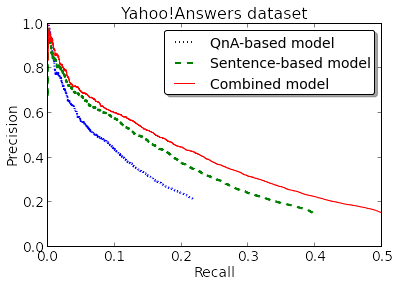
\includegraphics[width=0.99\textwidth]{img/cqarelextract_qa_vs_sent_ya}
    \label{figure:factoid:cqarelextract:pr_curve:ya}
\end{subfigure}
\begin{subfigure}[h]{0.45\textwidth}
    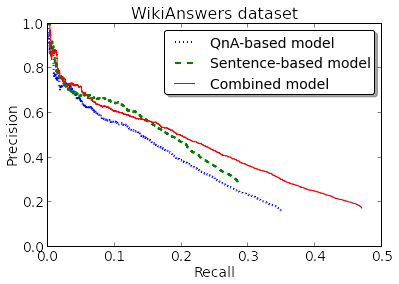
\includegraphics[width=0.99\textwidth]{img/cqarelextract_qa_vs_sent_wa}
    \label{figure:factoid:cqarelextract:pr_curve:wa}
\end{subfigure}
\begin{subfigure}[h]{0.45\textwidth}
    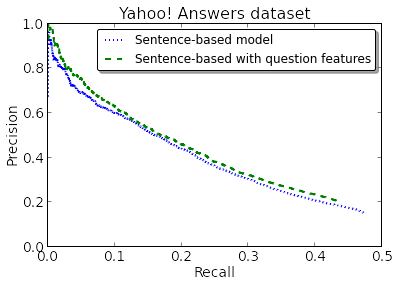
\includegraphics[width=0.99\textwidth]{img/cqarelextract_noqf_vs_qf}
    \label{figure:factoid:cqarelextract:noqf_vs_qf}
\end{subfigure}
\caption{Precision-Recall curves for QnA-based vs sentence-based models and sentence-based model with and without question features.}
\label{figure:factoid:cqarelextract:pr_curve}
\end{figure}

\begin{table}
\centering
\small
\begin{tabular}{p{4.7cm}|ccc|ccc}
& \multicolumn{3}{c|}{Yahoo! Answers} & \multicolumn{3}{c}{WikiAnswers}\\
& QnA & Sent. & Comb. & QnA & Sent. & Comb.\\
\hline
F-1 score & 0.219 & 0.276 & 0.310 & 0.277 & 0.297 & 0.332\\
Number of correct extractions & 3229 & 5900 & 7428 & 2804 & 2288 & 3779 \\
Correct triples not extracted by other model & 20.5\% & 56.5\% & - & 39.4\% & 25.8\% & - \\
\end{tabular}
\caption{Results for relation extraction of QnA-, sentence-based and combined models on Yahoo!~Answers and WikiAnswers datasets.}
\label{table:factoid:cqarelextract:results}
\end{table}

Results demonstrate that from 20.5\% to 39.4\% of correct triples extracted by the QnA-based model are not extracted by the baseline model, and the combination of both models is able to achieve higher precision and recall.
Unfortunately, comparison of the sentence-based model with and without question-based features (Figure~\ref{figure:factoid:cqarelextract:pr_curve}) did not show a significant difference.

\subsection{Analysis and Discussion}
\label{section:factoid:cqarelextract:analysis}

To get an idea of typical problems of the QnA-based model we sampled and manually judged extracted high confidence examples that are not present in Freebase (and thus are considered incorrect for precision-recall analysis).

The major reason (40\%) of false positive extractions is errors in entity linking.
For example: ``\textit{Who is Tim O'Brien? He was born in Austin on October 1, 1946}''.
The model was able to correctly extract [Tim O'Brien, date\_of\_birth, October 1, 1946], however, Tim O'Brien was linked to a wrong person.
In a number of cases (16\%) our discourse model turns out to be too simple and fails for answers, that mention numerous additional information, \eg ``\textit{How old is Madonna really? ...Cher was born on 20 May 1946 which makes her older that Madonna...}''.
A possible solution would be to either restrict QnA-based model to cases when no additional information is present or design a better discourse model with deeper analysis of the answer sentence and its predicates and arguments.
Some mistakes are due to distant supervision errors, for example for the music.composition.composer predicate our model extracts singers as well as composers (which are in many cases the same).

Of course, there are a number of cases, when our extractions are indeed correct but are either missing (33\%) or contradicting with Freebase (8\%).
An example of an extracted fact, that is missing in Freebase is ``\textit{Who is Wole Soyinka? He studied at the University College, Ibadan(1952-1954) and the University of Leeds (1954-1957)}'', and [Wole Soyinka, institution, University of Leeds] is currently not present in Freebase.
Contradictions with Freebase occur because of different precision levels (``pianist'' vs ``jazz pianist'', city vs county, \etc), different calendars used for dates or ``incorrect'' information provided by the user.
An example, when existing and extracted relation instance are different in precision is:``\textit{Who is Edward Van Vleck? Edward Van Vleck was a mathematician born in Middletown, Connecticut}'' we extract [Edward Van Vleck, place\_of\_birth, Middletown], however, the Freebase currently has the USA as his place of birth.

The problem of ``incorrect'' information provided in the answer is very interesting and worth special attention.
It has been studied in CQA research, \eg \cite{shah2010evaluating}, and an example of such QnA pair is: ``\textit{Who is Chandrababu Naidu? Nara Chandra Babu Naidu (born April 20, 1951)}''.
Other authoritative resources on the Web give April 20, 1950, as Chandrababu Naidu's date of birth.
This raises a question of trust to the provided answer and expertise of the answerer.
Many questions on CQA websites belong to the medical domain, \eg people asking advice on different health related topics.
How much can we trust the answers provided to extract them into the knowledge base?
We leave this question to the future work.

Finally, we have seen that only a small fraction of available QnA pairs was annotated with existing Freebase relations, which shows a possible limitation of Freebase schema.
A promising direction for future work is the automatic extraction of new predicates, which users are interested in and which can be useful to answer more future questions.

% \subsection{Summary}
% \label{section:factoid:cqarelextract:summary}

% In this section I described a model for relation extraction from QnA data, which is capable of predicting relations between entities mentioned in question and answer sentences.
% The experiments, conducted on 2 publicly available CQA datasets, showed that our model can extract triples not available to existing sentence-based techniques and can be effectively combined with them for better coverage of a knowledge base population system.

% =-=-=-=-=-=-=-=-=-=-Cqa Relation Extraction: End-=-=-=-=-=-=-=-=-=-=-=-=-=-=-

% =-=-=-=-=-=-=-=-=-=-=-=-=-=-Text2KB: Begin=-=-=-=-=-=-=-=-=-=-=-=-=-=-=-=-=-

\section{Text2KB: Augmenting Knowledge Base Question Answering with External Text Data}
\label{section:factoid:text2kb}

Existing relation extraction tools are not perfect, in particular, due to recall losses a lot of information is left behind.
Moreover, extractions contain a certain level of incorrect information due to precision losses.
Therefore, by applying relation extraction we are lowering the upper bound of the performance of an underlying question answering system.
An alternative approach is to keep the information in its raw unstructured format and design a way to use it along with KB.
In this section, I describe a novel factoid question answering system, that utilizes available textual resources to improve different stages of knowledge base question answering (KBQA).
This work was presented as a full paper at SIGIR 2016 conference~\cite{Savenkov:2016:KBE:2911451.2911536}.

KBQA systems must address three challenges, namely, question entity identification (to anchor the query process); candidate answer generation; and candidate ranking.
We will show that these challenges can be alleviated by the appropriate use of external textual data.
Entity identification seeds the answer search process, and therefore the performance of the whole system greatly depends on this stage~\cite{yao-scratch-qa-naacl2015}.
The question text is often quite short, may contain typos and other problems, that complicate entity linking.
Existing approaches are usually based on dictionaries that contain entity names, aliases and some other phrases, used to refer to the entities \cite{SPITKOVSKY12.266}.
These dictionaries are noisy and incomplete, \eg to answer the question \textit{``what year did tut became king?''} a system needs to detect a mention \textit{``tut''}, which refers to the entity \texttt{Tutankhamun}.
If a dictionary does not contain a mapping \textit{``tut''} $\rightarrow$ \texttt{Tutankhamun}, as happens for one of the state-of-the-art systems, it will not be able to answer the question correctly.
Such less popular name variations are often used along with full names inside text documents, for example, to avoid repetitions.
Therefore, we propose to look into web search results to find variations of question entity names, which can be easier to link to a KB (Figure~\ref{figure:factoid:text2kb:web_search_entitylink}).
This idea has been shown effective in entity linking for web search queries\footnote{\href{url}{http://web-ngram.research.microsoft.com/ERD2014/}} \cite{SMAPH_ERD:2014}.

\begin{figure}[t]
\centering
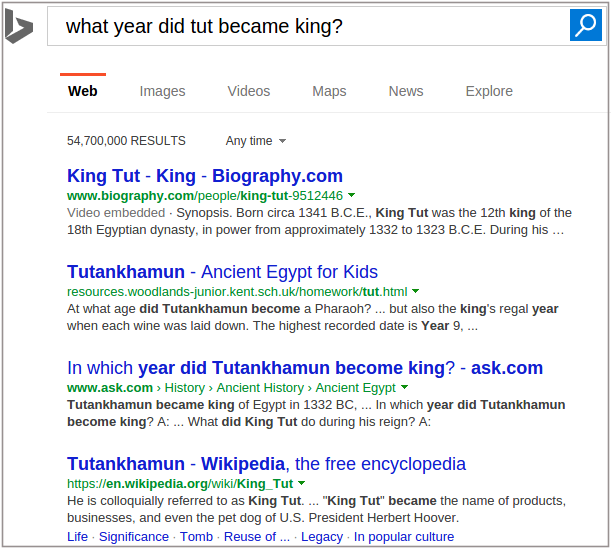
\includegraphics[width=0.75\textwidth]{img/web_search_entitylink}
\caption{Web search results for the question \textit{``what year did tut became king?''}, which mention both the full name of the king and the correct answer to the question.}
\label{figure:factoid:text2kb:web_search_entitylink}
\end{figure}

After question entities have been identified, answer candidates need to be generated and ranked to select the best answer.
A candidate query includes one or multiple triple patterns with predicates, corresponding to words and phrases in the question.
Existing knowledge base question answering approaches~\cite{bastmore:cikm:2015:aquu,BerantCFL13:sempre,BerantL14:parasempre,berant2015imitation,BordesCW14:emnlp,yao2014freebase} rely on a lexicon, learned from manually labeled training data, and supported by additional resources, such as question paraphrases \cite{BerantL14:parasempre} and weakly labeled sentences from a large text collection \cite{YaoD14}.
Such training data tends to be small compared to the number of different predicates in a KB, and therefore the coverage of these lexicons is limited.
By our estimate, in a popular WebQuestions KBQA dataset~\cite{BerantCFL13:sempre}, the answers to $\sim$5.5\% of test questions (112 out of 2032) involve a predicate that does not appear as a ground truth in the training set.
For example, the RDF triple \texttt{[Bigos, food.dish.type\_of\_dish1, Stew]} answers the question \textit{``what are bigos?''}, but no other examples in the training set involve this predicate.
In addition, a lexicon needs to cover all different ways a predicate can be asked about.
For example, questions \textit{``who did jon gosselin cheat with?''} and \textit{``who is the woman that john edwards had an affair with?''} are answered by the same KB predicate but use different language.
Therefore, the presence of the first question in a training set may not help to answer the second question.
On the other hand, traditional Text-QA systems benefit from the redundancy of the information on the Web, where the same facts are stated multiple times in many different ways~\cite{lin2007exploration}.
This increases the chances of a good lexical match between a question and answer statements, which makes even some relatively simple counting-based techniques quite effective~\cite{brill2002analysis}.
The model I developed adapts these ideas from text-based question answering for KBQA.

The general architecture and an example use case of Text2KB is presented on Figure~\ref{figure:factoid:text2kb:model}.
Text2KB is based on the information extraction approach to knowledge base question answering~\cite{YaoD14}, in particular, it extends the Aqqu system of H.Bast et al.~\cite{bastmore:cikm:2015:aquu}, which is one of the best performing open source KBQA system on the WebQuestions dataset.
The left part of the Figure~\ref{figure:factoid:text2kb:model} describes a typical architecture of IE-based KBQA systems, and the right part introduces additional external text data sources, namely Web search results, community question answering (CQA) data, and a collection of documents with detected KB entity mentions.
First, I describe the main stages of the information extraction approach to knowledge base question answering using Aqqu, the baseline system, as an example.

\begin{figure}[t]
\centering
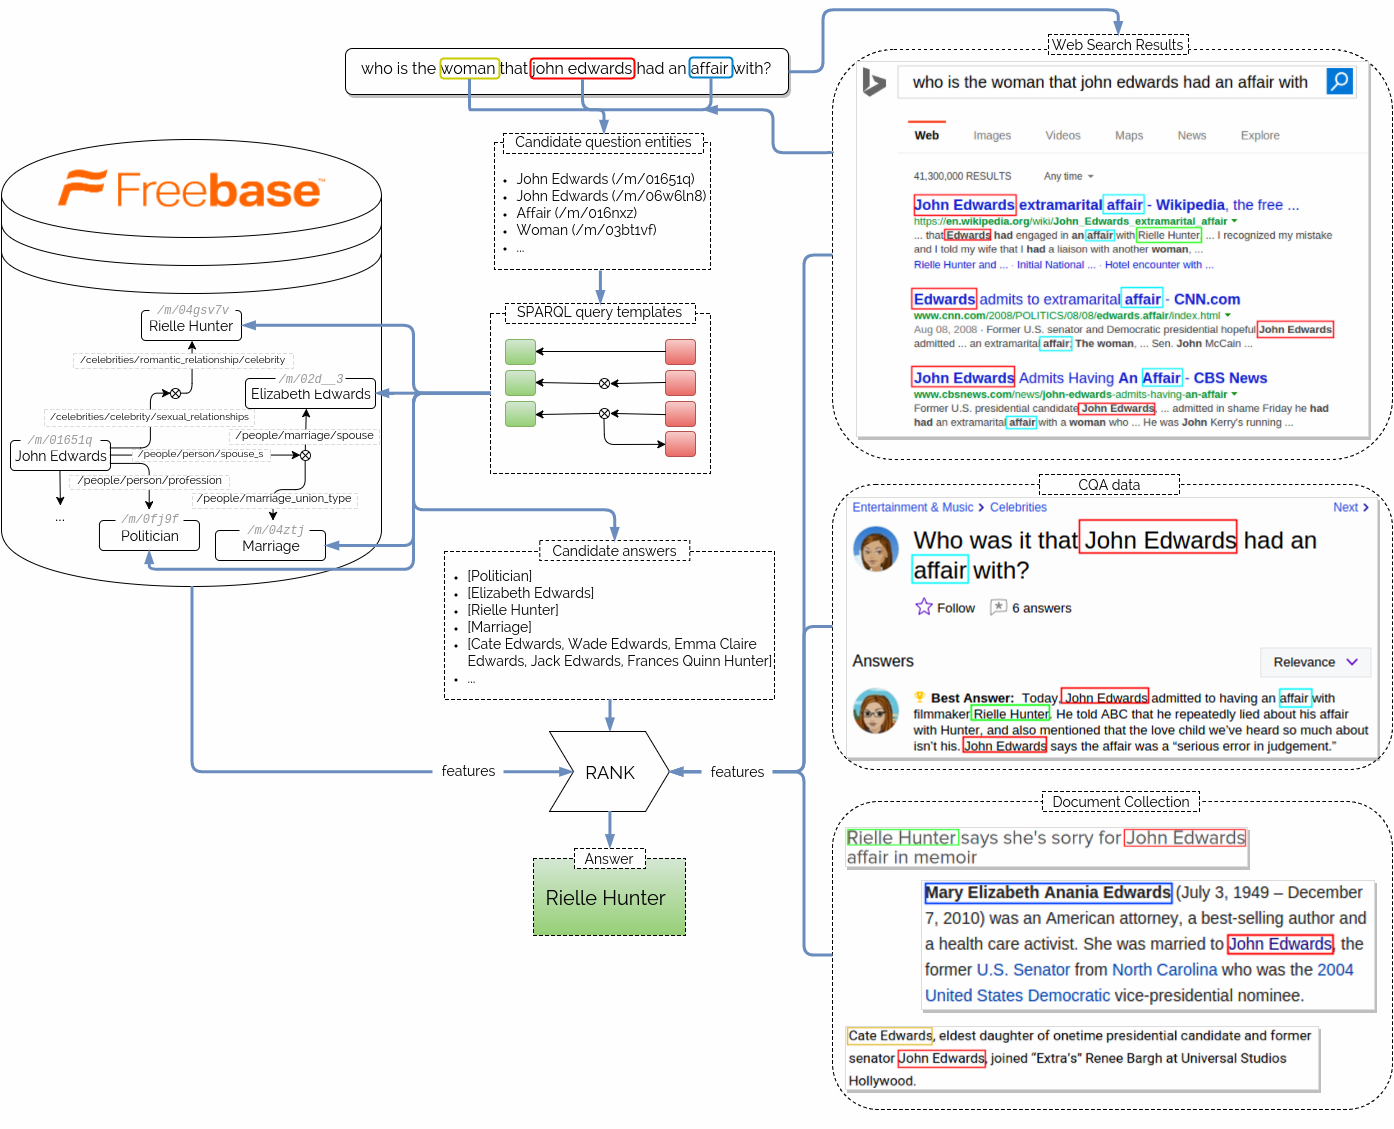
\includegraphics[width=\textwidth]{img/text2kb_model}
\caption{The architecture of the Text2KB Question Answering system.}
\label{figure:factoid:text2kb:model}
\end{figure}

\subsection{Baseline Approach}
\label{section:factoid:text2kb:baseline}

The first stage of the knowledge base question answering process is the identification of question topic entities, which are used as sources for the answer search process.
For concreteness, consider a question from the WebQuestions dataset \textit{``who is the woman that john edwards had an affair with?''}.
Here, the entity \texttt{John Edwards} with Freebase id \texttt{/m/01651q} is the main question entity.
However, Freebase contains millions of entities and it can be difficult to identify the topical ones (\eg entities \texttt{Woman} and \texttt{Affair} are also present in Freebase), or to disambiguate and choose between \texttt{John Edwards} a politician (\texttt{/m/01641q}), an American racing driver (\texttt{/m/06zs089}) and other people with the same name.
Aqqu considers all spans of question words under certain conditions on part of speech tags and uses an entity names lexicon \cite{SPITKOVSKY12.266} to map phrases to potential entities.
Most reported systems, including Aqqu, do not disambiguate entities at this stage, but rather keep a set of candidates along with some information about their popularities (\eg number of mentions in the collection), and mention scores $p(entity| mention\ text)$.

At the next stage, SPARQL query candidates are generated by exploring the neighborhood of the question topic entities using a predefined set of query templates.
Each query template has question entities, predicates and answer placeholders.
The majority of the answers in the WebQuestions dataset can be covered by just 3 templates (q\_entity - question entity, a\_entity - answer entity, cvt\_node - Freebase mediator node, which represents tuples with more than 2 arguments):
\\

\begin{minipage}{\linewidth}
\begin{lstlisting}[frame=single,basicstyle=\small]
SELECT DISTINCT ?a_entity {
   <q_entity> <predicate> ?a_entity .
}
\end{lstlisting}
\end{minipage}

\begin{minipage}{\linewidth}
\begin{lstlisting}[frame=single,basicstyle=\small]
SELECT DISTINCT ?a_entity {
   <q_entity> <predicate_1> ?cvt_node .
   ?cvt_node <predicate_2> ?a_entity .
}
\end{lstlisting}
\end{minipage}

\begin{minipage}{\linewidth}
\begin{lstlisting}[frame=single,basicstyle=\small]
SELECT DISTINCT ?a_entity {
   <q_entity_1> <predicate_1> ?cvt_node .
   ?cvt_node <predicate_2> <q_entity_2> .
   ?cvt_node <predicate_3> ?a_entity .
}
\end{lstlisting}
\end{minipage}

The first template retrieves a set of entities that are directly connected to the given question entity via a certain predicate.
The second template accounts for the presence of a mediator node, that groups together arguments of a multi-argument relation.
And the last template looks for cases when a question also mentions another argument of a multi-argument relation, \eg \texttt{Captain Kirk} and \texttt{Star Trek} for the question \textit{``who played captain kirk in star trek movie?''}.

Each query candidate is represented with a set of features, that includes the scores for linked question entities, various scores for matching between question term n-grams and query predicates, the size of the results list, \etc
The final stage of the question answering process is filtering and ranking.
The Aqqu system employs a pairwise learning-to-rank model, trained on part of the dataset.
For each pair of candidate answers, Aqqu creates an instance, which contains 3 groups of features: features of the first, the second candidate in the pair and the differences between the corresponding features of the candidates. Specifically, a Random Forest model is used in the provided Aqqu implementation. 
A pair where the first candidate is better than the second belongs to class +1, and -1 otherwise.
To reduce the number of pairs for the final ranking, Aqqu includes a simplified linear filtering model, which is trained to detect incorrect answers with high precision. 

In Text2KB we also introduced a couple of extensions to the original Aqqu system, which does not involve external text data.
We noticed that since Aqqu does not use information about the answer entity Freebase types, in many cases it returns an answer that is incompatible with the question: \eg state instead of county \etc
Therefore, we trained a model to return a score that measures compatibility between the question and answer entities, based on the entity notable types and question uni- and bi-grams as features, similar to Aqqu's relations score model.
A second extension introduced a new date range query template, which helps solve cases like \textit{``what team did david beckham play for in 2011?''}, where we need to look at the ranges of dates to determine whether an answer candidate satisfies the question.
\\

\begin{minipage}{\linewidth}
\begin{lstlisting}[frame=single,basicstyle=\small]
SELECT DISTINCT ?a_entity {
   <q_entity_1> <predicate_1> ?cvt_node .
   ?cvt_node <from_predicate> ?date_from .
   ?cvt_node <to_predicate> ?date_to .
   ?cvt_node <predicate_2> ?a_entity .
   FILTER ( <question_date> >= ?date_from AND
            <question_date> <= ?date_to )
}
\end{lstlisting}
\end{minipage}


\subsection{Text2KB Model}
\label{section:factoid:text2kb:model}

Text2KB improves the baseline knowledge base question answering model by utilizing textual resources on various stages of the pipeline.
Our model uses web search results to improve question analysis, \ie identify question topic, and extract additional features to support generated answer candidates.
Question-answer pairs from CQA archives are used to learn associations between question words and KB predicates, and score candidate SPARQL queries.
Finally, a text collection annotated with KB entity mentions is used to build a language model for entity pairs, and generate answer ranking features.

\textbf{Web search results for question understanding and answer ranking.}
Traditional TextQA systems rely on search results to retrieve relevant documents, which are then used to extract answers to users' questions.
Relevant search results mention question entities multiple times and in various forms, which can be helpful for entity linking \cite{SMAPH_ERD:2014}.
Furthermore, retrieved document set often contains multiple occurrences of the answer, which can be a strong signal for candidate ranking~\cite{lin2007exploration}.

To obtain related web search results, Text2KB issues the question as a query to a search engine\footnote{In our experiments, we use the Bing Web Search API \href{url}{https://www.microsoft.com/cognitive-services/en-us/bing-web-search-api} and local Wikipedia search using Lucene}, extracts top 10 result snippets and the corresponding documents.
Next, Text2KB uses Aqqu entity linking module to detect KB entity mentions in both snippets and documents.

Question text provides only a limited context for entity disambiguation and linking; additionally, the entity name can be misspelled or an uncommon variation used.
This complicates the task of entity identification, which is the foundation of KB question answering process.
Fortunately, web search results help with these problems, as they usually contain multiple mentions of the same entities and provide more context for disambiguation.
Text2KB uses the search result snippets to \textit{expand} the set of detected question entities.
More specifically, we count the frequencies of each entity mentioned in search snippets, and most popular ones with names similar to some of the question terms are added to the list of topical entities.
The goal of this similarity condition is to keep only entities that are likely mentioned in the question text and filter out related, but different entities.
To estimate the similarity between a name and question tokens, we use Jaro-Winkler string distance.
An entity is added to the list of question entities if at least one of its tokens $e_t$ has high similarity with one of the question tokens $q_t$ excluding stopwords ($Stop$):
$$max_{e_t \in M \backslash Stop, q_t \in Q \backslash Stop} 1 - dist(e_t, q_t) \geq 0.8$$

The information stored in KBs can also be present in other formats, \eg text statements.
For example, on Figure \ref{figure:factoid:text2kb:web_search_entitylink} multiple search snippets mention the date when Tutankhamun became a king.
TextQA systems use such passages to extract answer to users' questions.
However, text may not provide sufficient context information about the mentioned entities, and systems have to infer the useful details, \eg entity types, which can be problematic \cite{yih2014semantic}.
On the other hand, KBQA systems can utilize all the available KB knowledge about the entities in a candidate answer and would benefit from additional text-based information to improve ranking.
More specifically, Text2KB proceeds as follows (full list of features is given in Table~\ref{table:factoid:text2kb:features}):

\begin{enumerate}
\item Precompute term and entity IDFs. We used Google n-grams corpus to approximate terms IDF by collection frequencies and available ClueWeb Freebase entity annotations\footnote{\href{url}{http://lemurproject.org/clueweb09/FACC1/}} to compute entity IDF scores.
\item Each snippet $s_i$ and document $d_i$ are represented by two TF-IDF vectors of lowercased tokens ($t_{s_i}$ and $t_{d_i}$) and mentioned entities ($e_{s_i}$ and $e_{d_i}$).
\item In addition, vectors of all snippets and all documents are merged together to form combined token and entity vectors: $t_{\cup s_i}$, $t_{\cup d_i}$, $e_{\cup s_i}$ and $e_{\cup d_i}$.
\item Each answer candidate $a_j$ is also represented as TF-IDF vector of terms (from entity names), and entities: $t_{a_j}$ and $e_{a_j}$
\item Cosine similarities between answer and each of 10 snippet and document vectors are computed: $\cos(t_{s_i}, t_{a_j})$, $\cos(t_{d_i}, t_{a_j})$ and $\cos(e_{s_i}, e_{a_j})$, $\cos(e_{d_i}, e_{a_j})$.
We use the average score and the maximum score as features.
\item We also compute answer similarities with the combined snippet and document vectors: $\cos(t_{\cup s_i}, t_{a_j})$, $\cos(e_{\cup s_i}, e_{a_j})$, $\cos(t_{\cup d_i}, t_{a_j})$, $\cos(e_{\cup d_i}, e_{a_j})$.
\end{enumerate}

\textbf{CQA data for matching questions to predicates.}
Recall that a major challenge in KBQA is that natural language questions do not easily map to entities and predicates in a KB.
An established approach for this task is supervised machine learning, which requires labeled examples of questions and the corresponding answers to learn this mapping, which can be expensive to construct.
Researchers have proposed to use weakly supervised methods to extend a lexicon with mappings learned from \textit{single sentence statements} mentioning entity pairs in a large corpus \cite{YaoD14}.
However, the language used in questions to query about a certain predicate may differ from the language used in statements.
In Section~\ref{section:factoid:cqarelextract} we demonstrated how distant supervision can be applied to question-answer pairs from CQA archives for a related task of information extraction for knowledge base completion.
In a similar way, we use weakly labeled collection of question-answer pairs to compute {\em associations} between question terms and predicates to \textit{extend} system's lexicon (Figure~\ref{figure:factoid:text2kb:cqa_example}).
We emphasize that this data does not replace the mappings learned from single sentence statements, which are already used by our baseline system, but rather introduces the new ones learned from the CQA data.

\begin{figure}[t]
\centering
\fbox{
 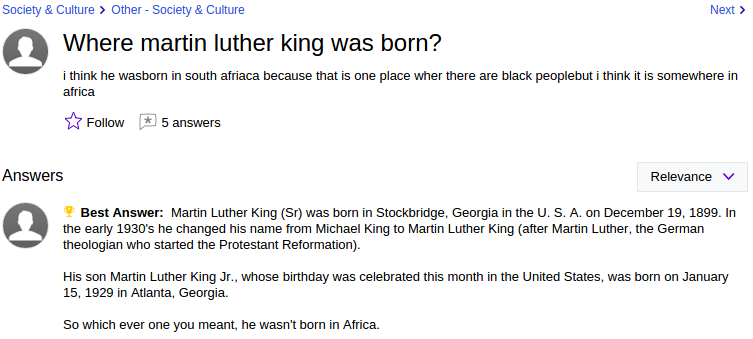
\includegraphics[width=0.7\textwidth]{img/cqa_example}
}
\caption{Example of a question and answer pair from Yahoo! Answers CQA website.}
\label{figure:factoid:text2kb:cqa_example}
\end{figure}

For our experiments, we use 4.4M questions from Yahoo! WebScope L6 dataset\footnote{\href{url}{https://webscope.sandbox.yahoo.com/}}.
Question and answer texts were run through an entity linker, that detected mentions of Freebase entities.
Next, we use distant supervision assumption to label each question-answer pair with predicates between entities mentioned in the question and in the answer.
These labels are used to learn associations between question terms and predicates by computing pointwise mutual information scores (PMI) for each term-predicate pair.
Examples of scores for some terms are given in Table~\ref{table:factoid:text2kb:cqa_npmi}.

\begin{table}[t]
\centering
\begin{tabular}{rp{8.5cm}l}
Term & Predicate & PMI\\
\hline
born & \texttt{people.person.date\_of\_birth} & 3.67\\
 & \texttt{people.person.date\_of\_death} & 2.73\\
 & \texttt{location.location.people\_born\_here} & 1.60\\
\hline
kill & \texttt{people.deceased\_person.cause\_of\_death} & 1.70\\
& \texttt{book.book.characters} & 1.55\\
\hline
currency & \texttt{location.country.currency\_formerly\_used} & 5.55 \\
& \texttt{location.country.currency\_used} & 3.54 \\
\hline
school & \texttt{education.school.school\_district} & 4.14 \\
& \texttt{people.education.institution} & 1.70\\
& \texttt{sports.school\_sports\_team.school} & 1.69 \\
\hline
illness & \texttt{medicine.symptom.symptom\_of} & 2.11\\
& \texttt{medicine.decease.causes} & 1.68\\
& \texttt{medicine.disease.treatments} & 1.59\\
\hline
win & \texttt{sports.sports\_team.championships} & 4.11\\
& \texttt{sports.sports\_league.championship} & 3.79\\
\end{tabular}
\caption{Examples of term-predicate pairs with high PMI scores, computed using distant supervision from a CQA collection.}
\label{table:factoid:text2kb:cqa_npmi}
\end{table}

In Text2KB we evaluate candidate answer predicates by using the association (\eg PMI) scores between predicates and the question terms (missing pairs are given a score of 0).
The minimum, average and maximum of these values are used as features to represent a candidate answer.
Such associations data can be sparse, we also use pretrained word2vec word embeddings\footnote{\href{url}{https://code.google.com/p/word2vec/}}.
We compute predicate embeddings by taking a weighted average of term vectors from predicate's PMI table.
Each term vector is weighted by its PMI value (terms with a negative score are skipped).
Then, we compute cosine similarities between predicate vector and each of the question term vectors and take their minimum, average, maximum as features.
Finally, we average embeddings of question terms and compute its cosine similarity with the predicate vector (full list of features is given in Table~\ref{table:factoid:text2kb:features}).

\textbf{Estimating entity associations using a semantically annotated text collection.}
A key step for ranking candidate answers is to estimate whether the question and answer entities are related in a way asked in the question.
Existing KBQA approaches usually focus on scoring the mappings between question phrases and KB concepts from a candidate SPARQL query.
However, textual data can provide another angle on the problem, as question and answer entities are likely to be mentioned together somewhere in text passages.
For example, in the bottom right corner of Figure~\ref{figure:factoid:text2kb:model} we can see some passages that mention a pair of people, and the context of these mentions explains the nature of the relationships.
This data can be viewed as additional edges in a KB, which connect pairs of entities and have associated language models, estimated from text phrases, that mention these entities.
Such edges do not have to coincide with the existing KB edges and can connect arbitrary pairs of entities, that are mentioned together in the text, therefore extend the KB.

We use the ClueWeb12 corpus with existing Freebase entity annotations and count different terms that occur in the context of a mention of a pair of different entities (we only consider mentions within 200 characters of each other).
To compute this unigram language model we use the terms separating the entities, as well as the terms within a small window (\eg 100 characters) before and after the entity mentions.
A small sample of this data is presented in Table~\ref{table:factoid:text2kb:clueweb_entitypairs_langmodel}.

\begin{table}
\centering
\small
\begin{tabular}{rlp{7cm}}
Entity 1 & Entity 2 & Frequent terms\\
\hline
 & Rielle Hunter & campaign, affair, mistress, child, former ...\\
 & Cate Edwards & daughter, former, senator, courthouse, greensboro, eldest ...\\
John Edwards & Elizabeth Edwards & wife, hunter, campaign, affair, cancer, rielle, husband ...\\
 & Frances Quinn & daughter, john, rielle, father, child, former, paternity...\\
 \hline
\end{tabular}
\caption{Example of entity pairs along with the most popular terms mentioned around the entities in ClueWeb12 collection.}
\label{table:factoid:text2kb:clueweb_entitypairs_langmodel}
\end{table}

We use this data to compute candidate ranking features as follows.
Consider question words $Q$ and an answer candidate, which contains a question entity $e_1$ and one or more answer entities $e_2$.
For each answer candidate, we compute a language model score:
$$p(Q|e_1, e_2) = \prod_{t\in Q} p(t | e_1, e_2)$$
and use the minimum, average and maximum over all answer entities as features.
To address the sparsity problem, we again use embeddings, 
\ie for each entity pair a weighted (by counts) average embedding vector of terms is computed and minimum, average and maximum cosine similarities between these vectors and question token embeddings are used as features (full list of features is given in Table~\ref{table:factoid:text2kb:features}).

\textbf{Internal text data to enrich entity representation.}
In addition to external text data, many knowledge bases, including Freebase, contain text data as well, \eg Freebase includes a description paragraph from Wikipedia for many of its entities.
These text fragments provide a general description of entities, which may include information relevant to the question \cite{Sun:2015:ODQ:2736277.2741651}.
For completeness, we include them in our system as well.
Each entity description is represented by a vector of tokens, and a vector of mentioned entities.
We compute cosine similarities between token and entity vectors of the question and description of each of the answers and use the minimum, average and maximum of the scores as features.

The final list of text-based features used in Text2KB model is presented in Table~\ref{table:factoid:text2kb:features}.

\begin{table}[h!]
\centering
\small
\begin{tabular}{r|p{8cm}}
Data Source & Feature\\
\hline
Search results (\texttt{Wiki} or \texttt{Web}) & - number of entity mentions in search results \\
 & - max and average tf-idf cosine similarity between answer and search snippets/documents \\
 & - max and average embeddings cosine similarity between question tokens and search snippets/documents \\
CQA data (\texttt{CQA}) & - sum, average, minimum and maximum PMI scores between question tokens and answer predicates \\
 & - sum, average, minimum and maximum embeddings cosine similarity scores between question tokens and PMI-weighted answer predicates tokens \\
Text collection (\texttt{CL}) & - min, max and average entity-pair language model score for question topic and answer entities \\
 & - min, max and average entity-pair embeddings score for question topic and answer entities \\
\end{tabular}
\caption{The list of text-based features used in the Text2KB model.}
\label{table:factoid:text2kb:features}
\end{table}

\subsection{Experimental Results}
\label{section:factoid:text2kb:eval}

This section reports the experimental setup, including the dataset and metrics, as well as the main methods compared for evaluating the performance of our Text2KB system. Additionally, we describe a series of ablation studies to analyze the contribution of different system components.

\textbf{Methods Compared}.
We compare our system, Text2KB, to state-of-the-art approaches, notably:
\begin{itemize}[noitemsep]
\item{\textbf{Aqqu}}: a state-of-the-art baseline KBQA system~\cite{bastmore:cikm:2015:aquu}, described in Section~\ref{section:factoid:text2kb:baseline}.
\item{\textbf{Text2KB(Web search)}}: Our Text2KB system, using the Bing search engine API over the Web. 
\item{\textbf{Text2KB(Wikipedia search)}}: Our Text2KB system, using the standard Lucene search engine over the February 2016 snapshot of the English Wikipedia, in order to validate our system without the potential ``black-box'' effects of relying on a commercial Web search engine (Bing) and changing corpus (Web).
\item{\textbf{STAGG}}: One of the best\footnote{It was the best result published before summer 2016, \ie the camera-ready version of my paper, describing Text2KB system.} current KBQA systems~\cite{yih:ACL:2015:STAGG} as measured on the WebQuestions dataset.
\end{itemize}
Additionally, other previously published results on WebQuestions are included to provide context for the improvements introduced by our Text2KB system.

\textbf{Datasets}.
I followed the standard evaluation procedure for the WebQuestions dataset and used the original 70-30\% train-test split (3,778 training and 2,032 test instances). Within the training split, 10\% was set aside for validation to tune the model parameters and only the best-performing set of parameters selected on the validation data was used to report the results on the official test split.

\textbf{Evaluation Metrics}. 
Recent papers using the WebQuestions dataset have primarily used the average F1-score as the main evaluation metric, defined as:
$avg\ F1 = \frac{1}{|Q|} \sum_{q \in Q} f1(a^*_q, a_q)$
$$f1(a^*_q, a_q) = 2\frac{precision(a^*_q,a_q) recall(a^*_q,a_q)}{precision(a^*_q,a_q) + recall(a^*_q,a_q)}$$
$precision(a^*_q, a_q)=\frac{|a^*_q \cap a_q|}{|a_q|}$ and $recall(a^*_q, a_q) = \frac{|a^*_q \cap a_q|}{|a^*_q|}$, $a^*_q$ and $a_q$ are correct and given answers to the question q, which can be lists of entities.
Additionally, I report average precision and recall, to gain a better understanding of the trade-offs achieved by different methods.

\begin{table}[t]
\centering
\small
\begin{tabular}{rp{1.9cm}p{1.7cm}p{1.9cm}p{1.2cm} }
System & $\overline{Recall}$ & $\overline{Precision}$ & F1 of $\overline{P}$ \& $\overline{R}$ & $\overline{F1}$ \\
\hline
OpenQA \cite{Fader:2014:OQA:2623330.2623677} & - & - & - & 0.35 \\
YodaQA \cite{baudivs2015yodaqa} & - & - & - & 0.343 \\
\hline
Jacana \cite{YaoD14} & 0.458 & 0.517 & 0.486 & 0.330\\
SemPre \cite{BerantCFL13:sempre} & 0.413 & 0.480 & 0.444 & 0.357\\
Subgraph Embed \cite{BordesCW14:emnlp} & - & - & 0.432 & 0.392\\
ParaSemPre \cite{BerantL14:parasempre} & 0.466 & 0.405 & 0.433 & 0.399\\
Kitt AI \cite{yao-scratch-qa-naacl2015} & 0.545 & 0.526 & 0.535 & 0.443\\
AgendaIL \cite{berant2015imitation} & 0.557 & 0.505 & 0.530 & 0.497\\
DepLambda \cite{reddy2016transforming} & 0.611 & 0.490 & 0.544 & 0.503 \\
STAGG \cite{yih2014semantic} & 0.607 & 0.528 & 0.565 & 0.525\\
Textual Evidence\cite{xu2016enhancing} & - & - & - & 0.533 \\
FMN \cite{jain2016question} & \textbf{0.649} & \textbf{0.552} & \textbf{0.597} & \textbf{0.557}\\
\hline
Aqqu (baseline) \cite{bastmore:cikm:2015:aquu} & 0.604 & 0.498 & 0.546 & 0.494\\
Text2KB$_{Wiki Search}$ & \textbf{0.632}$_{(+4.6\%)}^*$  & 0.498 & 0.557$_{(+2.0\%)}^*$ & 0.514$_{(+4.0\%)}^*$ \\
Text2KB$_{Web Search}$ & \textbf{0.635}$_{(+5.1\%)}^*$ & 0.506$_{(+1.6\%)}^*$ & \textbf{0.563}$_{(+3.1\%)}^*$ & \textbf{0.522}$_{(+5.7\%)}^*$ \\
\end{tabular}
\caption{Average performance metrics of the Text2KB system on WebQuestions dataset compared to the existing approaches. The differences of scores marked * from the baseline Aqqu system are significant with p-value $<$ 0.01.}
\label{table:factoid:text2kb:webquestions_results}
\end{table}

\textbf{Main Results.}
The results of existing approaches and our Text2KB system are presented in Table~\ref{table:factoid:text2kb:webquestions_results}.
We should note, that text-based QA systems typically return a ranked list of answers, whereas many answers on WebQuestions dataset are lists, which complicates the comparison between KBQA and text-based systems.
The result reported for YodaQA system is the F1 score at position 1.
As we can see, Text2KB significantly improves over the baseline system.

\textbf{Data Source and Features Contribution}.
To analyze the contribution of the features and data sources I introduced, I report results from a series of ablation studies. For convenience, I introduce the following short-hand notations for different components of our system:

\begin{itemize}[noitemsep]
\item \texttt{T} - notable type score model as a ranking feature
\item \texttt{DF} - date range filter-based query template
% \item TF - using notable type based filter
\item \texttt{WebEnt} - using web search result snippets for question entity identification
\item \texttt{WikiEnt} - using wikipedia search result snippets for question entity identification
\item \texttt{Web} - using web search results for feature generation
\item \texttt{Wiki} - using wikipedia search results for feature generation
\item \texttt{CQA} - using CQA-based \texttt{[question term, KB predicate]} PMI scores for feature generation
\item \texttt{CW} - features, computed from entity pairs language model, estimated on ClueWeb
\end{itemize}

In the results table I will use the notation \texttt{+$<$comp$>$} for a system with a certain component added, and \texttt{-$<$comp$>$} when it is removed.
For example, the baseline system will be denoted as ``\texttt{Aqqu}''.
The same system with additional date range filter query templates and notable types score model is denoted as ``\texttt{Aqqu +DF+T}'', which represents the same system as ``\texttt{Text2KB -WebEnt-Web-CQA-CL}'' (we will call it Text2KB (base)).
Our full system ``\texttt{Text2KB}'' can be also denoted as ``\texttt{Aqqu +DF+T+WebEnt+Web+CQA+CL}''.

First, I analyze the improvements introduced by different components of the system (Table~\ref{table:factoid:text2kb:ablation:entities_vs_features}).
As we can see, additional date range filters and notable types model (\texttt{Aqqu+DF+T}) are responsible for an increased recall and a drop in precision compared to the baseline model.
Features generated from Wikipedia search results, CQA data and ClueWeb entity pair language models (\texttt{+Wiki+CQA+CL}) improve average F1 by 0.007 (+1.4\%) compared to the base model, adding entity linking using Wikipedia search results improves results even more (+3\%).

Web search results (\texttt{+Web+CQA+CL}) turned out to be more helpful than Wikipedia results (\texttt{+Wiki+CQA+CL}), which is natural since Wikipedia is a subset of the web.
This was one of the reasons we did not combine Wikipedia and Web search together.
Finally, entity linking and all text-based features combined achieves an even higher score, proving that their contributions are independent.

I now analyze the contribution of the different data sources.
I will remove a group of web search, CQA or Clueweb-based features and see how the performance of the whole system changes (Table~\ref{table:factoid:text2kb:ablation:features}).
As we can see, all data sources have an impact on the system performance, and web search results based features provide the most useful signal for answer ranking.

Figure~\ref{figure:factoid:text2kb:ablation:feature_importances} plots a subset of features ranked by their Gini index-based importance scores.
The figure supports the observation that web search results features are the most useful, however, other text data sources also contribute to the improvement.

\begin{table}
\centering
\begin{tabular}{rlll}
System & Recall & Prec & F1 \\
\hline
\texttt{Aqqu} & 0.604 & 0.498 & 0.494\\
\texttt{Text2KB (base) = Aqqu+DF+T} & 0.617 & 0.481 & 0.499 \\
\hline
\texttt{+Wiki+CQA+CL} & 0.623 & 0.487 & 0.506 \\
\texttt{+WikiEnt +Wiki+CQA+CL} & 0.632 & 0.498 & 0.514 \\
\hline
\texttt{+WebEnt} & 0.627 & 0.492 & 0.508 \\
\texttt{+Web+CQA+CL} & 0.634 & 0.497 & 0.514 \\
\texttt{+WebEnt +Web+CQA+CL} & 0.635 & 0.506 & 0.522 \\
\end{tabular}
\caption{Average Recall, Precision (Prec), and F1 of Aqqu and Text2KB system with and without different components. +A means that a component A is added to the Text2KB (base) system.}
\label{table:factoid:text2kb:ablation:entities_vs_features}
\end{table}

\begin{table}[h]
\centering
\begin{tabular}{rlll}
System & Recall & Prec &  F1 \\
\hline
\texttt{Text2KB} (Web search) & 0.635 & 0.506 & 0.522 \\
\hline
% THIS PART ANSWERS HOW GOOD ARE EACH OF THE PROPOSED DATASETS
% extent_cqa_clueweb_dates_typemodel_rf100.log : -web
\texttt{Text2KB -Web} & 0.633 & 0.496 & 0.513 \\
% extent_web_clueweb_dates_typemodel_rf100.log : -cqa
\texttt{Text2KB -CQA} & 0.642 & 0.499 & 0.519 \\
% extent_web_cqa_dates_typemodel_rf100.log : -clueweb
\texttt{Text2KB -CL} & 0.644 & 0.505 & 0.523 \\
\hline
% extent_web_dates_typemodel_rf100.log : -clueweb-cqa
\texttt{Text2KB -CQA-CL} & 0.642 & 0.503 & 0.522 \\
% extent_clue_dates_typemodel_rf100.log : -web-cqa
\texttt{Text2KB -Web-CQA} & 0.631 & 0.498 & 0.514 \\
% extent_cqa_dates_typemodel_rf100.log : -web-clueweb
\texttt{Text2KB -Web-CL} & 0.622 & 0.493 & 0.508 \\
%\hline
% extent_web_cqa_clueweb_dates_types_typemodel_rf100.log : everything, including type filters
%\texttt{Text2KB} & 0.6354 & 0.5059 & 0.5223 \\
\end{tabular}
\caption{Average Recall, Precision (Prec), and F1 of Text2KB with and without features based on web search results, CQA data and ClueWeb collection.}
\label{table:factoid:text2kb:ablation:features}
\end{table}

\begin{figure*}
\centering
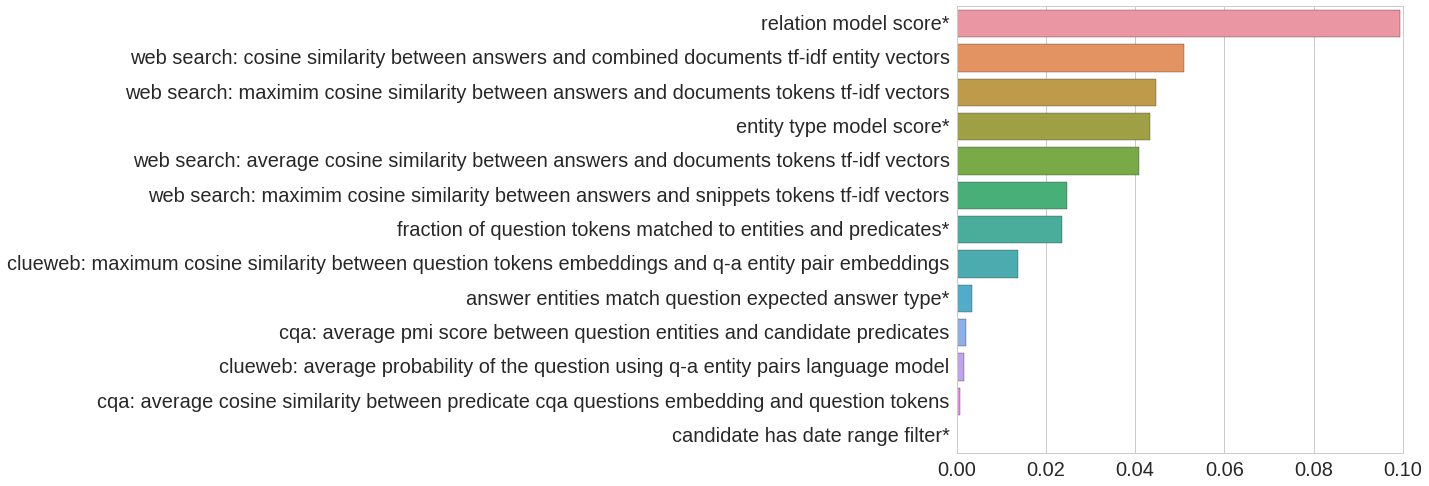
\includegraphics[width=\textwidth]{img/feature_importances}
\caption{A plot of Gini importances of different features of our answer ranking random forest model (features marked * are not text-based and are provided for comparison).}
\label{figure:factoid:text2kb:ablation:feature_importances}
\end{figure*}

In summary, Text2KB significantly outperforms the baseline system, and each of the introduced components contributes to this improvement.
Web search results data turned out to be the most useful resource, and it significantly improves the quality by helping with question entity identification and candidate ranking.
Next, I analyze the system performance in more detail and investigate factors for future extension.

\subsection{Analysis}
\label{section:factoid:approaches:text2kb:analysis}

I now investigate how Text2KB compares to other systems on the same benchmark; then, I investigate in depth the different error modes, which helps identify the areas of most substantial future improvements.

I took an existing KBQA system and demonstrated that by combining evidence from a knowledge base and external text resources we can boost the performance.
A reasonable question is whether the same approach will be helpful for other systems, \eg the best system at the moment of our paper publication -- STAGG~\cite{yih:ACL:2015:STAGG}.
STAGG differs from the baseline system Aqqu in the components: entity linking algorithm, a set of query templates and ranking methods.
Therefore, my approach is ``orthogonal'' to these improvements and should be helpful for STAGG as well.
To support this claim, I made an experiment to combine answers of STAGG and Text2KB.
One of the advantages of the former is its set of filters, that restricts list results to entities of certain type, gender, \etc
Therefore, I combined answers of STAGG and Text2KB using a simple heuristic: I chose to use the answer returned by STAGG if the number of answer entities is less than in the Text2KB answer, otherwise, I used the answer of Text2KB.
Table~\ref{table:factoid:text2kb:combine_stagg} gives the results of the experiment, and as we can see the combination achieves a slightly better average F1 score.
Alternatively, we can look at the Oracle combination of the systems, which always selects the answer with the higher F1.
As we can see such a combination results in a performance of 0.606, which is much higher than either of the systems.

\begin{table}
\centering
\begin{tabular}{rl}
System  & avg F1 \\
\hline
Text2KB & 0.522\\
STAGG~\cite{yih:ACL:2015:STAGG} & 0.525\\
Text2KB + STAGG & 0.532 (+1.3 \%) \\
Text2KB + STAGG (Oracle) & 0.606 (+15.4 \%) \\
\end{tabular}
\caption{Average F1 for combinations of Text2KB and STAGG using a simple heuristic based on the length of the answer list and Oracle upper bound.}
\label{table:factoid:text2kb:combine_stagg}
\end{table}

As I mentioned earlier, answers to 112 of the test questions in the WebQuestions dataset involve predicates that were not observed in the training set, which may be a problem for approaches that rely on a trained lexicon.
I evaluated both systems on these questions, and indeed the performance is very low, \ie the average F1 score of Text2KB is 0.1640 compared to 0.1199 for STAGG\footnote{Unfortunately, the number of questions is too low to show statistical significance (p-value=0.16) of the difference.}.

\begin{figure}
\centering
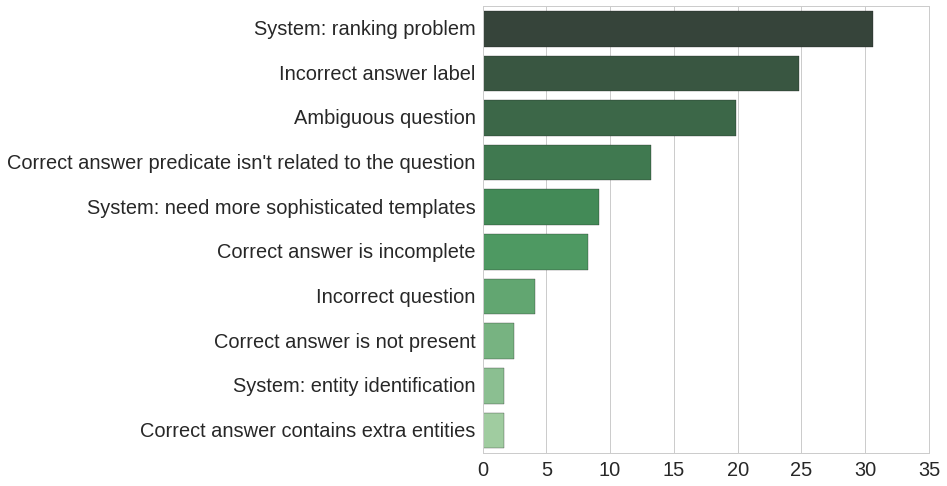
\includegraphics[width=0.7\textwidth]{img/error_analysis}
\caption{Distribution of problems with questions, where Text2KB returns an answer with F1$<$1.}
\label{figure:factoid:text2kb:error_analysis}
\end{figure}

To get better insights into the problems that remain, I collected 1219 questions for which Text2KB did not return a completely correct answer, \ie F1 score $<$ 1.
I manually looked through a couple of hundreds of these examples and grouped the problems into several clusters (Figure~\ref{figure:factoid:text2kb:error_analysis}).

As we can see candidate ranking is still the major problem, and it accounts for $\sim31\%$ of the cases.
The second problem is incorrect ground truth labels (almost 25\% of reported errors).
Another set of questions has incomplete or overcomplete ground truth answer list.
Typical examples are questions asking for a list of movies, books, landmarks, \etc
The ground truth answer usually contains $\sim10$ entities, whereas the full list is often much larger.
This seems to be an artifact of the labeling process, where the answer was selected from the Freebase entity profile page, which shows only a sample of 10 entities, while the rest are hidden behind the ``N values total'' link.
About 20\% of the questions are ambiguous, \ie questions have no strict 1-1 correspondence with any of the predicates and can be answered by multiple ones without any obvious preferences.
For example, the question \textit{``what did hayes do?''} can be answered by profession, occupied position or some other achievements.
Another problem is when there is no predicate that answers the question.
For example, the question \textit{``what do people in france like to do for fun?''} does not have a good match among the facts stored in Freebase.
The ground truth entity \texttt{Cycling} comes from the list Olympic sport competitions country participated\footnote{\texttt{olympics.olympic\_participating\_country.athletes}}.

Text2KB components were quite effective in resolving some of the problems.
Web search results helped identify the right question topical entity in a number of cases, \eg \textit{``what did romo do?''} mentions only the last name of the Dallas Cowboys quarterback and the baseline system were unable to map it to the right entity.
Web search results provides more than enough evidence that ``\textit{romo}'' refers to \texttt{Tony Romo}.
However, there is a number of loses, introduced by added unrelated entities.
For example, the entity \texttt{I Love Lucy} was added for the question \textit{``what was lucille ball?''}, because the term \textit{lucy} had high similarity with \textit{lucille}.
A portion of these problems can be fixed by a better entity linking strategy, \eg \cite{SMAPH_ERD:2014}.
An interesting example, when external text resources improved the performance is the question \textit{``what ship did darwin sail around the world?''}.
This is actually a hard question because the ship entity is connected to the \texttt{Charles Darwin} entity through the ``knownFor'' predicate along with some other entities like \texttt{Natural selection}.
% \footnote{\texttt{user.lindenb.default\_domain.scientist.known\_for}
Thus, the predicate itself is not related to the question, but nevertheless, the name of the ship \texttt{HMS Beagle} is mentioned multiple times in the web search results, and entity pair model computed from ClueWeb also has high scores for the terms ``ship'' and ``world''.

There are several major reasons for the loses, introduced by features based on external text resources.
Some entities often mentioned together and therefore one of them gets high values of co-occurrence features.
For example, the baseline system answered the question \textit{``when did tony romo got drafted?''} correctly, but since \texttt{Tony Romo} is often followed by \texttt{Dallas Cowboys}, Text2KB ranked the team name higher.
Another common problem with our features is an artifact of entity linking, which works better for names and often skips abstract entities, like professions.
For example, the correct answer to the question \textit{``what did jesse owens won?''} is an entity with the name \texttt{Associated Press Male Athlete of the Year}, which is rarely mentioned or it is hard to find such mentions.
Some problems were introduced by a combination of components.
For example, for \textit{``where buddha come from?''} a topical entity \texttt{Buddhism} was introduced from search results, and it generated \texttt{Gautama Buddha} as one of the answer candidates.
This answer was ranked the highest due to a large number of mentions in the search results.

% \subsection{Summary}
% \label{section:factoid:approaches:text2kb:summary}

In summary, in this section, I demonstrated that unstructured text resources can be effectively utilized for knowledge base question answering to improve query understanding, candidate answer generation and ranking.
Textual resources can help KBQA system mitigate the problems of matching between knowledge base entities and predicates and textual representation of the question.

Unfortunately, Text2KB does not help with the problem of knowledge base incompleteness, \ie my system will not be able to respond to the question, which refers to an entity, a predicate or a fact, which is missing in a KB.
Section~\ref{section:factoid:evinets} describes a neural network framework, that naturally combines evidence of different nature for factoid question answering.

% =-=-=-=-=-=-=-=-=-=-=-=-=-=-Text2KB: End=-=-=-=-=-=-=-=-=-=-=-=-=-=-=-=-=-


% =-=-=-=-=-=-=-=-=-=-=-=-=-=-EviNets: Begin=-=-=-=-=-=-=-=-=-=-=-=-=-=-=-=-=-
\section{EviNets: Joint Model for Text and Knowledge Base Question Answering}
\label{section:factoid:evinets}

%Unstructured textual and structured KB resources have their own advantages and disadvantages, that could compensate each other.
%Prior approaches to the problem of combining textual and structured knowledge base data either process data sources using separate pipelines and merge the results~\cite{baudivs2015yodaqa,ferrucci2010building}, extract structured knowledge from text~\cite{Agichtein:2000:SER:336597.336644,Dong:2014:KVW:2623330.2623623,MintzBSJ09}, convert both data sources into a semi-structured format~\cite{Fader:2014:OQA:2623330.2623677}, extend knowledge bases with information extracted from text~\cite{elbassuoni2009language,yahya2016question} or  enrich text with some knowledge about the mentioned entities~\cite{Sun:2015:ODQ:2736277.2741651}.
%Unfortunately, such approaches usually sacrifice some potentially useful information available in the data sources.

A critical task for question answering is the final answer selection stage, which has to combine multiple signals available about each answer candidate.
Most of the recent works in QA have focused on the problem of semantic matching between a question and candidate answer sentences~\cite{he2016pairwise,rao2016noise,yang2016anmm}.
The datasets used in these works, such as Answer Sentence Selection Dataset~\cite{wang2007jeopardy} and WikiQA~\cite{yang2015wikiqa}, typically contain a relatively small set of sentences, and the task is to select those that state the answer to the question.
However, for many questions, a single sentence does not provide sufficient information, and it may not be reliable in isolation. At the same time,
the redundancy of information in large corpora, such as the Web, has been shown useful to improve information retrieval approaches to QA~\cite{clarke2001exploiting}.

% An alternative approach for factoid question answering uses knowledge bases, which are collections of \texttt{[subject, predicate, object]} triples.
% Recent development of large scale open domain knowledge bases, such as dbPedia~\cite{auer2007dbpedia}, Freebase~\cite{Bollacker:2008:FCC:1376616.1376746} and WikiData~\cite{vrandevcic2014wikidata}, motivated research in knowledge base question answering, \eg ~\cite{BerantCFL13:sempre,yih:ACL:2015:STAGG,bastmore:cikm:2015:aquu} and many others.
% However, KBs are inherently incomplete~\cite{Dong:2014:KVW:2623330.2623623}, and do not have sufficient information to answer many other questions~\cite{Fader:2014:OQA:2623330.2623677}.


One approach for joint representation of diverse information is embedding into a low-dimensional space, \ie as achieved by various neural network architectures.
In particular, Memory Networks~\cite{sukhbaatar2015end} and their extensions~\cite{miller2016key} use embeddings to represent relevant data as memories, and summarize them into a single vector, therefore losing information about answers provenances.

In this section, I describe \textit{EviNets}, a novel neural network architecture for factoid question answering, which provides a unified framework for aggregating evidence, supporting answer candidates.
Given a question, \textit{EviNets} retrieves a set of relevant pieces of information, \eg sentences from a corpora or knowledge base triples, and extracts mentioned entities as candidate answers.
All the evidence signals are then embedded into the same vector space, scored and aggregated using multiple strategies for each answer candidate.
Experiments on the TREC QA, WikiMovies and new Yahoo!~Answers datasets demonstrate the effectiveness of the proposed approach, and its ability to handle both unstructured text and structured KB triples as evidence.
This work was published as a short paper at the Annual Meeting of the
Association for Computational Linguistics 2017~\cite{savenkov_evinets17}.

\subsection{Model and Architecture}
\label{section:factoid:evinets:model}

\begin{figure}[t]
\centering
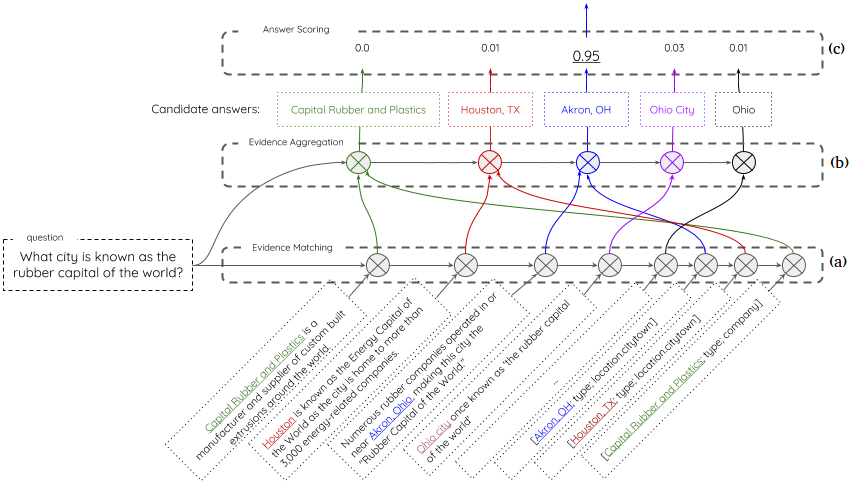
\includegraphics[width=\textwidth]{img/EviNet}
\caption{The architecture of EviNets Neural Networks for combining textual and KB evidence in factoid question answering.}
\label{figure:factoid:evinet:model}
\end{figure}

The high level architecture of \textit{EviNets} is illustrated in Figure~\ref{figure:factoid:evinet:model}.
For a given question, we extract potentially relevant information, \eg sentences from documents retrieved from text corpora using a search system.
Next, we can use an entity linking system, such as TagMe~\cite{ferragina2010tagme}, to identify entities mentioned in the extracted information, which become candidate answers.
\textit{EviNets} can further incorporate additional supporting evidence, \eg textual description of candidate answer entities, and potentially useful KB triples, such as types~\cite{Sun:2015:ODQ:2736277.2741651}.
Finally, question, answer candidates and supporting evidence are given as input to the \textit{EviNets} neural network.

\begin{figure}[t]
\centering
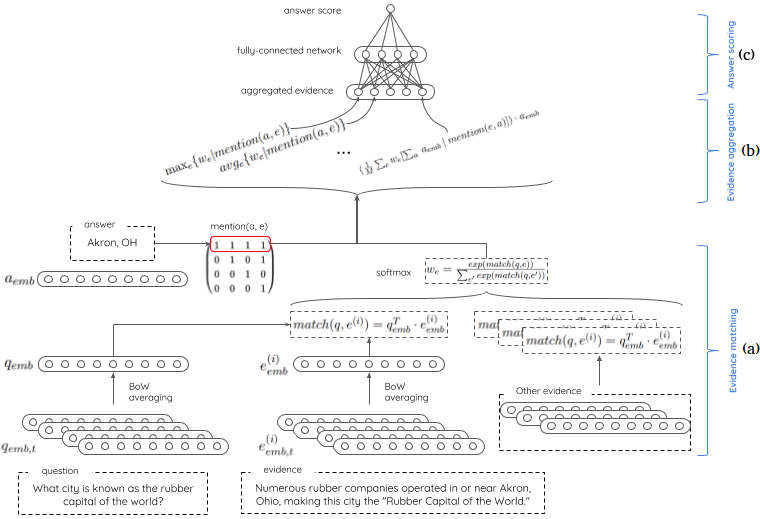
\includegraphics[width=\textwidth]{img/EviNetLayers}
\caption{Layer-wise structure of the EviNets Neural Networks framework for factoid question answering. Evidence matching (a), aggregation (b) and answer scoring (c) stages correspond to those in Figure~\ref{figure:factoid:evinet:model}.}
\label{figure:factoid:evinet:layers}
\end{figure}

Let us denote a question by $q$, and $\{q_t\in~R^{|V|}\}$, as a one-hot encoding of its tokens from a fixed vocabulary $V$.
$a_i$ is a candidate answer from the set $A$, and we will assume, that each answer is represented as a single entity.
For each question, we have a fixed set $E=E_{text} \cup E_{KB}$ of evidence statements $e^{(i)}, i=1..M$, and their tokens $e_t^{(i)}$.
A boolean function $mention:~A\times E\rightarrow\{0, 1\}$ provides the information about which answer candidates are mentioned in which evidences.
Individual tokens $q_t, a_i, e_t^{(i)}$ are translated into the embedding space using a matrix $W_{D\times~|V|}$, where $D$ is the dimension of the embeddings, \ie $q_{emb,t}~=~Wq_t$, $a_{emb,i}~=~Wa_t$ and $e^{(i)}_{emb,t}~=~We^{(i)}_t$.
In the experiments, I use the same matrix for questions, evidence, and answers.
KB entities are considered to be individual tokens, while predicates and type names are tokenized into constituent words, \ie by splitting on underscore and dot characters for Freebase predicates.
A layer-wise architecture of \textit{EviNets} is displayed on Figure~\ref{figure:factoid:evinet:layers}.
The evidence matching module ((a) on Figures~\ref{figure:factoid:evinet:model} and \ref{figure:factoid:evinet:layers}) estimates the relevance of each statement in the memory, and computes their weights using the softmax function.
The evidence aggregation module (b) uses multiple ways to compute the aggregated statistics of evidences, mentioning each answer candidate.
Finally, the answer scoring module (c) uses a fully connected network to predict a score for each answer candidate.
EviNets selects the answer with the highest score as the final response.

\subsubsection{Evidence Matching Module}

Evidence matching is responsible for estimating the relevance of each of the pieces of evidence to the question, i.e., $w_e~=~softmax(match(q, e))$.
The function \textit{match(q, e)} can be implemented using any of the recently proposed semantic similarity estimation architectures\footnote{e.g., see the ACL Wiki on Question\_Answering\_(State\_of\_the\_art).}.
One of the simplest approaches is to average question and each evidence token embeddings and score the similarity using the dot product: $q_{emb} = \frac{1}{L_q}\sum_t q_{emb,t}$ and $e^{(i)}_{emb} = \frac{1}{L_e}\sum_t e^{(i)}_{emb,t}$ and $match(q, e^{(i)}) = q^T_{emb} \cdot e^{(i)}_{emb}$.

\subsubsection{Evidence Aggregation Module}

\begin{table}[h!]
\centering
\small
\begin{tabular}{p{5.2cm}|p{7.8cm}}
Evidence Feature & Description \\
\hline
Maximum evidence score mentioning the answer & $\max_e \{w_e | mention(a, e)\}, e\in E,E_{text}~or~E_{KB}$ \\
Average evidence score mentioning the answer & $avg_e \{w_e | mention(a, e)\}, e\in E,E_{text}~or~E_{KB}$ \\
Sum of evidence scores mentioning the answer & $\sum_e \{w_e | mention(a, e)\}, e\in E,E_{text}~or~E_{KB}$ \\
Number of mentions & $\sum_e \{1 | mention(a, e)\}, e\in E_{text}$ \\
Weighted memory similarity to the question & $(\frac{1}{M}\sum_i w_e e^{(i)}_{emb})\cdot q_{emb}$\\
Weighted memory similarity to the answer~\cite{sukhbaatar2015end} & $(\frac{1}{M}\sum_i w_e e^{(i)}_{emb})\cdot a_{emb}$ or $R^T(\frac{1}{M}\sum_i w_e e^{(i)}_{emb} + q_{emb}) \cdot a_{emb}$, where $R_{D\times~D}$ is a rotation matrix \\
Weighted memory answer mentions similarity to the answer~\cite{miller2016key} & $(\frac{1}{M}\sum_e w_e [\sum_a~a_{emb}~|~mention(e, a)]) \cdot a_{emb}$ \\
\end{tabular}
\caption{Signals used in \textit{EviNets} to aggregate evidence in support for each of the answer candidates $a$.}
\label{table:factoid:evinet:aggregation}
\end{table}

After all the evidence signals have been scored, \textit{EviNets} aggregate the support for each answer candidate.
Table~\ref{table:factoid:evinet:aggregation} summarizes the aggregation features used.
With these features, \textit{EviNets} captures different aspects, \ie how well individual sentences match the question, how frequently the candidate is mentioned and how well a set of answer evidences covers the information requested in the question.

\subsubsection{Answer Scoring Module}

Finally, \textit{EviNets} uses the aggregated signals to predict the answer scores, to rank them, and to return the best candidate as the final answer to the question.
For this purpose, we use two fully-connected neural network layers with the ReLU activation function, with 32 and 8 hidden units respectively.
The model was trained end-to-end by optimizing the cross entropy loss function using the Adam algorithm~\cite{kingma2014adam}.

\subsection{Experimental Evaluation}
\label{section:factoid:evinet:eval}

\begin{table}
\small
\centering
\begin{tabular}{lp{9cm}}
Dataset & Example Questions \\
\hline
\textbf{TREC QA} & Where is the highest point in Japan? \\
1236 train & What is the coldest place on earth? \\
202 test & Who was the first U.S. president to appear on TV?\\
\hline
\textbf{WikiMovies} & what films did Ira Sachs write? \\
96185 train & what films does Claude Akins appear in? \\
10000 dev & the movie Victim starred who? \\
9952 test & what type of film is Midnight Run? \\
\hline
\textbf{Yahoo! Answers} & What is Elvis's hairstyle called? \\
1898 train & Who is this kid in Mars Attacks? \\
271 dev & who invented denim jeans? \\
542 test & who's the woman on the progressive.com commercials? \\
\end{tabular}
\caption{Statistics of the TREC QA, WikiMovies and Yahoo!~Answers factoid datasets.}
\label{table:factoid:evinet:datasets}
\end{table}


To test our framework we used TREC QA~\cite{Sun:2015:ODQ:2736277.2741651}, WikiMovies~\cite{miller2016key} benchmarks and the new Yahoo!~Answers dataset\footnote{available for research purposes at \href{url}{http://ir.mathcs.emory.edu/software-data/}} derived from factoid questions posted on the CQA website (Table~\ref{table:factoid:evinet:datasets}).
In all experiments, embeddings were initialized with 300-dimensional vectors pre-trained with Glove~\cite{pennington2014glove}.
Embeddings for multi-word entity names were obtained by averaging the word vectors of constituent words.

\subsubsection{Baselines}
\label{section:factoid:evinet:eval:baselines}

As baselines for different experiments depending on availability and specifics of a dataset we considered the following methods: 
\begin{itemize}[noitemsep,nolistsep]
\item IR-based QA systems: \textit{AskMSR}~\cite{brill2002analysis} and \textit{AskMSR+}~\cite{tsai2015web}, which select the best answer based on the frequency of entity mentions in retrieved text snippets. 
\item KBQA systems: \textit{SemPre}~\cite{BerantCFL13:sempre} and \textit{Aqqu}~\cite{bastmore:cikm:2015:aquu}, which identify possible topic entities of the question, and select the answer from the candidates in the neighborhood of these entities in a KB.
\item Hybrid system \textit{QuASE}~\cite{Sun:2015:ODQ:2736277.2741651} detects mentions of knowledge base entities in text passages, and uses the types and description information from the KB to support answer selection.
\item Hybrid system \textit{Text2KB}~\cite{Savenkov:2016:KBE:2911451.2911536}, which uses textual resources to improve different stages of the KBQA pipeline, described in Section~\ref{section:factoid:text2kb}.
\item Memory Networks: \textit{MemN2N}~\cite{sukhbaatar2015end} and \textit{KV MemN2N}~\cite{miller2016key} represent relevant information with embeddings, and summarize the memories into a single vector using the soft attention mechanism. Additionally, KV MemN2N splits memories into key-value pairs, where keys are used for matching against the question, and values are used to summarize the memories.
\end{itemize}


\subsubsection{TREC QA dataset}
\label{section:factoid:evinet:eval:trecqa}

The TREC QA dataset is composed of factoid questions, which can be answered with an entity, and were used in TREC 8-12 question answering tracks.
Similarly to~\cite{Sun:2015:ODQ:2736277.2741651} we used web search (using the Microsoft Bing Web Search API) to retrieve top 50 documents, parsed them, extracted sentences and ranked them using tf-idf similarity to the question.
To compare our results with the existing state-of-the-art, we used the same set of candidate entities as used by the QuASE model.
We note that the extracted evidence differs between the models, and we were unable to match some of the candidates to our sentences.
For text+kb experiment, just as QuASE, we used entity descriptions and types from Freebase knowledge base.

Table~\ref{table:factoid:evinet:eval:trecqa} summarizes the results.
\textit{EviNets} achieves competitive results on the dataset, beating KV MemN2N by $13\%$ in F1 score, and, unlike QuASE, does not rely on expensive feature engineering and does not require any external resources to train.

\begin{table}
\centering
\begin{tabular}{lrrr}
Method & P & R & F1 \\
\hline
SemPre & 0.157 & 0.104 & 0.125 \\
Text2KB & 0.287 & 0.287 & 0.288 \\
AskMSR+ & 0.493 & 0.490 & 0.491 \\
QuASE (text) & 0.550 & 0.550 & 0.550 \\
QuASE (text+kb) & 0.579 & \textbf{0.579} & \textbf{0.579} \\
\hline
MemN2N & 0.333 & 0.328 & 0.330 \\
KV MemN2N & 0.517 & 0.500 & 0.508 \\
EviNets (text) & 0.580 & 0.560 & 0.569 \\
EviNets (text+kb) & \textbf{0.585} & 0.564 & 0.574 \\
\end{tabular}
\caption{Precision, Recall and F1 of KB- and Text-based question answering methods on the TREC QA dataset. The improvements over the Key-Value memory networks are statistically significant at p-value $<$ 0.01.}
\label{table:factoid:evinet:eval:trecqa}
\end{table}

\subsubsection{WikiMovies dataset}
\label{section:factoid:evinet:eval:wikimovies}

The WikiMovies dataset contains questions in the movies domain along with relevant Wikipedia passages and the OMDb knowledge base.
Since KVMemN2N already achieves an almost perfect result answering the questions using the KB, we focus on using the provided movie articles from Wikipedia.
We followed the preprocessing procedures described in~\cite{miller2016key}.
Unlike TREC QA, where there are often multiple relevant supporting pieces of evidence, answers in the WikiMovies dataset usually have a single relevant sentence, which, however, mentions multiple entities.
To help the model distinguish the correct answer, and explore its abilities to encode structured and unstructured data, we generated additional \textit{entity type} triples.
For example, if an entity $e$ appears as an object of the predicate \texttt{directed\_by} in OMDb, we added the \texttt{[e, type, director]} triple.
As baselines, we used MemN2N and KV MemN2N models, and the results are presented in Table~\ref{section:factoid:evinet:eval:wikimovies}.
As we can see, with the same setup using individual sentences as evidence/memories \textit{EviNets} significantly outperforms the KV MemN2N model by $27\%$.
Moreover, the proposed approach can effectively incorporate additional entity type RDF triples, and significantly improve the performance over the text-only version.
It is important to emphasize that the best-reported results of memory networks were obtained using \textit{entity-centered windows} as memories, which requires special pre-processing and increases the number of memories.
Additionally, these models used \textit{all} of the KB entities as candidate answers, whereas \textit{EviNets} relies only on the mentioned ones, which is a more scalable scenario for open-domain question answering, where it is not realistic to score millions of candidate answers in real-time.

\begin{table}
\centering
\begin{tabular}{lr}
Method & Accuracy \\
\hline
MemN2N (wiki windows) & 0.699* \\
KV MemN2N (wiki windows) & 0.762* \\
\hline
AskMSR (entities) & 0.314 \\
KV MemN2N (wiki sent) & 0.524 \\
EviNets (wiki sent) & 0.616  \\
EviNets (wiki sent + entity types) & \textbf{0.667} \\
\end{tabular}
\caption{Accuracy of EviNets and baseline models on the WikiMovies dataset. The results marked * are obtained using a different setup, \ie they use pre-processed entity window memories, and the whole set of entities as candidates.}
\label{section:factoid:evinet:eval:wikimovies}
\end{table}

\subsubsection{New Yahoo! Answers factoid questions dataset}
\label{section:factoid:evinet:eval:yahoo}

Yahoo! recently released a dataset with search queries, which lead to clicks on factoid Yahoo!~Answers questions, identified as questions with the best answer containing less than 3 words and a Wikipedia page as the specified source of information\footnote{L27 dataset \href{url}{https://webscope.sandbox.yahoo.com}}.
This dataset contains 15K queries, which correspond to 4725 unique Yahoo!~Answers questions (Table~\ref{table:factoid:evinet:datasets}).
We took these questions, and mapped answers to KB entities using the TagMe entity linking library~\cite{ferragina2010tagme}.
We filtered out questions, for which no answer entities with a good confidence\footnote{A minimum  $\rho$ score of 0.2 from TagMe was required.} were identified, \eg date answers, and randomly split the rest into training, development and test sets, with 2711 questions in total.
Similarly to the TREC QA experiments, we extracted textual evidence using Bing Web Search API, by retrieving top 50 relevant documents, extracting the main content blocks, and splitting them into sentences.
We applied the TagMe entity linker to the extracted sentences, and considered all entities of mentions with the confidence score above the 0.2 threshold as candidate answers.
For candidate entities we also retrieved relevant KB triples, such as entity types and descriptions, which extended the original pool of evidences.

\begin{table}
\centering
\begin{tabular}{p{6cm}rrr}
Method & P & R & F1 \\
\hline
Aqqu & 0.116 & 0.117 & 0.116 \\
Text2KB & 0.170 & 0.170 & 0.170 \\
AskMSR (entities) & 0.175 & 0.319 & 0.226 \\
\hline
MemN2N & 0.072	& 0.131 & 0.092 \\
KV MemN2N & 0.126 & 0.228 & 0.162 \\
\hline
% EviNets (text) & 0.210 & 0.383 & 0.271\small{$_{+67\%}$} \\
% EviNets (text+kb) & \textbf{0.226} & \textbf{0.409} & \textbf{0.291}\small{$_{+79\%}$} \\
EviNets (text) & 0.210 & 0.383 & 0.271 \\
EviNets (text+kb) & \textbf{0.226} & \textbf{0.409} & \textbf{0.291} \\
\hline
Oracle & 0.622 & 1.0 & 0.767 \\
\end{tabular}
\caption{Precision, Recall and F1 of different methods on Yahoo! Answers factoid QA dataset. The Oracle performance assumes candidate answers are ranked perfectly and is bound by the performance of the initial retrieval step.}
\label{table:factoid:evinet:eval:yahoo}
\end{table}

Table~\ref{table:factoid:evinet:eval:yahoo} summarizes the results of \textit{EviNets} and some baseline methods on the created Yahoo!~Answers dataset.
As we can see, knowledge base data is not enough to answer most of these questions, and a state-of-the-art KBQA system Aqqu gets only 0.116 precision.
Adding textual data helps significantly, and Text2KB improves the precision to 0.17, which roughly matches the results of the AskMSR system, that ranks candidate entities by their popularity in the retrieved documents.
EviNets significantly improves over the baseline approaches, beating AskMSR by $28\%$ and KV MemN2N by almost $80\%$ in F1 score.
Using text along with KB evidence gave higher performance metrics, boosting F1 from 0.271 to 0.291.

In the above-mentioned experiments we used bag-of-words representation for questions and evidence, and a reasonable question is whether more complicated methods could achieve higher results.
Table~\ref{table:factoid:evinet:eval:yahoo_bilstm} compares bag-of-words representation with bidirectional LSTM~\cite{WangN15}.
On Yahoo!~Answers dataset BOW representation showed better performance, which is most likely due to a relatively low size of the dataset for the variety of questions present there.

\begin{table}
\centering
\begin{tabular}{lrrr}
Method & P & R & F1 \\
\hline
EviNets (text+kb): BOW & 0.226 & 0.409 & 0.291 \\
EviNets (text+kb): biLSTM & 0.196 & 0.356 & 0.252 \\
\end{tabular}
\caption{Precision, Recall and F1 of EviNets with bag-of-words and bidirectional LSTM representations of questions and evidence.}
\label{table:factoid:evinet:eval:yahoo_bilstm}
\end{table}


\subsection{Discussion}
\label{section:factoid:evinet:discussion}

\textit{EviNets}, described in this section, is a neural network for question answering, which encodes and aggregates multiple evidence signals to select answers.
Experiments on TREC QA, WikiMovies and Yahoo!~Answers datasets demonstrate that \textit{EviNets} can be trained end-to-end to use both the available textual and knowledge base information.
EviNets improves over the baselines, both in cases when there are many or just a few relevant pieces of evidence, by helping build an aggregate picture and distinguish between candidates, mentioned together in a relevant memory, as is the case for WikiMovies dataset.
The results of the experiments also demonstrate that EviNets can incorporate signals from different data sources, \eg adding KB triples helps to improve the performance over text-only setup.
As a limitation of the approach and a direction for future research, \textit{EviNets} could be extended to support dynamic evidence retrieval, which would allow retrieving additional answer candidates and evidence as needed.

% =-=-=-=-=-=-=-=-=-=-=-=-=-=-EviNets: End=-=-=-=-=-=-=-=-=-=-=-=-=-=-=-=-=-

\section{Summary}
\label{section:factoid:summary}

This Chapter introduced several approaches for combining unstructured, semi-structured and structured data sources to improve factoid question answering.
Relation extraction from question-answer pairs aims at filling some gaps in KB fact coverage.
The experiments show, that we can use distant supervision to extract factual knowledge from community question answering archives and increase the recall of the existing sentence-based relation extraction techniques.
However, extraction techniques are not perfect and suffer from both precision and recall losses.
As an alternative strategy, we can use semantic annotations of entity mentions in a text to connect knowledge base and textual data.
Such annotation allows to quickly find relevant textual resources and improve KBQA methods, as demonstrated by Text2KB model, or use both data sources together, as pieces of supporting evidence for generated answer candidates.
Diverse information can be mapped into the embedding space and aggregated together with a neural network architecture, such as \textit{EviNets}.

Factoid questions represent just a part of user information needs. Many problems require a more elaborate response, such as a sentence, list of instructions or, in general, a passage of text.
Such questions are usually referred to as non-factoid questions and they will be the focus of Chapter~\ref{chapter:non-factoid}.



% Example of the algorithm package.

% \begin{algorithm}[ht!]
% \caption[How to write a thesis]{How to write a thesis}
% \begin{algorithmic}[1]
%  \REQUIRE Some good ideas, nice figures, and some time to type it.
%  \ENSURE A nice thesis.
% \WHILE{thesis is not done}
% \STATE{keep working on it}
% \STATE{do not sleep}
% \STATE{have enough fast food at home}
% \ENDWHILE
% \FORALL{committee members}
% \STATE{take them for a beer}
% \STATE{show them the nice figures}
% \IF{they all like it}
% \STATE{\label{line:print}}{print everything and turn it in}
% \ELSE
% \REPEAT
% \STATE{\label{line:beer}}{give them another beer}
% \UNTIL{they like it}
% \ENDIF
% \ENDFOR
% \end{algorithmic}
% \end{algorithm}
		\clearpage
\chapter{Improving Non-factoid Question Answering}
\label{chapter:non-factoid}

Factoid questions studied in Chapter~\ref{chapter:factoid} represent only a fraction of user information needs, and there are many other types of questions, which cannot be answered with entity names or dates.
The variety of user information needs is reflected in different types of questions, that people post to community question answering websites~\cite{harper2010question,ignatova2009annotating,Liu:2008:USA:1599081.1599144}.
Such questions usually require a longer response, \eg a paragraph of text, list of instructions, \etc
For the majority of such questions, modern search engines still return the ``10 blue links'', and delegate the task of digging into the information and extracting relevant pieces of knowledge to the user, which can be quite time-consuming.
In this Chapter, I focus on improving question answering for such generic information needs.

Previous research on non-factoid question answering either focused on a small subset of questions (\eg definition questions~\cite{hildebrandt2004answering}), or considered this as a problem of ranking existing answers in CQA archives, which can be reused to answer new questions~\cite{carmel2000eresponder,Shtok:2012:LPA:2187836.2187939}.
To advance the research in the area of automatic question answering for a general class of user information needs in 2015 TREC started a series of LiveQA evaluation campaigns\footnote{\href{url}{http://trec-liveqa.org}}.
The TREC LiveQA track task is to develop a real-time system to answer real user questions, that are posted live to Yahoo!~Answers\footnote{\href{url}{http://answers.yahoo.com/}} community question answering platform.

This chapter describes the methods and ideas I implemented in a system, that participated in 2015 and 2016 versions of the track.
The system uses a combination of semi-structured information, \ie question-answer pairs from different CQA platforms, with unstructured information, which can be extracted from regular web documents.
The former strategy of retrieving similar previously posted questions was shown to be quite effective~\cite{carmel2000eresponder,Shtok:2012:LPA:2187836.2187939}, as it allows a system to return a naturally looking answer in cases when a good match was found.
However, many similar questions are formulated differently, which complicates the retrieval problem, additionally, many incoming information needs are still unique and there are simply no similar questions in the archive.
In this case a system can extract its answer from potentially relevant passages of regular web documents.
In Section~\ref{section:non-factoid:system} I will describe the architecture of \textit{EmoryQA}: the system I developed to participate in the TREC LiveQA shared task.

Despite the indisputable improvements in automatic answer selection\footnote{\href{url}{http://aclweb.org/aclwiki/index.php?title=Question\_Answering\_(State\_of\_the\_art)}}, the analysis of results of TREC LiveQA 2015 task demonstrated, that we still have a big gap in performance between human and automatic question answering.
Mistakes, that were made by trained machine learning models for answer passage selection, could be easily spotted by a human in fractions of a second even when a person does not have enough expertise in the area of the question.
To build on this observation, we looked into how an automatic system can integrate crowdsourcing to improve its performance.
More specifically, we propose to use feedback of a crowd of workers to extend the answers pool and obtain quality labels for generated answer candidates.
Section~\ref{section:non-factoid:crowdsourcing} describes the design of the crowdsourcing component and the results of TREC LiveQA 2016, which demonstrated its effectiveness for near real-time question answering.

In summary, the main contributions of this chapter include:
\begin{itemize}
\item An open-source state-of-the-art automatic question answering system for a general class of user information needs, evaluated at TREC LiveQA 2015 and 2016 tracks.
The architecture of the system and evaluation results were published in TREC conference proceedings~\cite{savenkov2015trec,savenkov2016trec}.
\item A novel hybrid question answering system, that incorporates a crowdsourcing module, but still operates in near real-time, and significantly improves performance over the pure automatic approach.
This work was presented as a full paper at HCOMP 2016~\cite{savenkov_crqa2016}.
\end{itemize}

% -=-=-=-=-=-=-=-=-=-=-=-= LiveQA : Begin -=-=-=-=-=-=-=-=-=-=-=
\section{Ranking Answers and Web Passages for Non-factoid Question Answering}
\label{section:non-factoid:system}

In this section, I describe the architecture of \textit{EmoryQA} (Figure~\ref{figure:non-factoid:emoryqa}), the automatic question answering system, which combines semi-structured data from CQA archives and unstructured web document passages to cover a variety of questions that users have.

\begin{figure}
    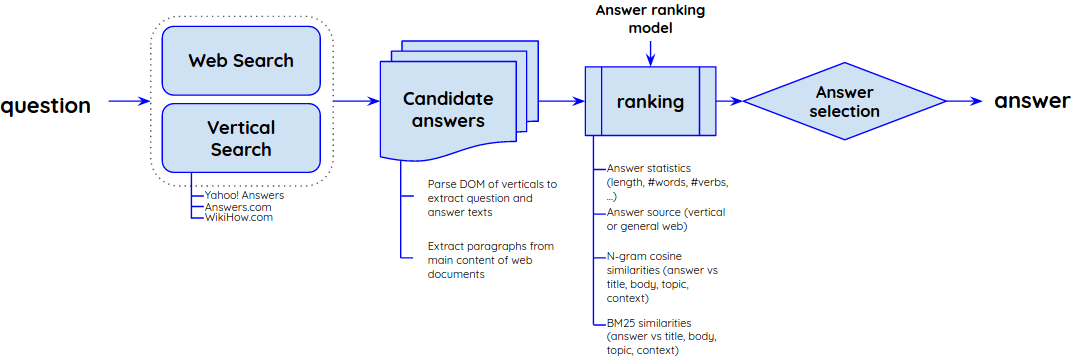
\includegraphics[width=\textwidth]{img/emoryqa_design}
    \caption{Architecture of the EmoryQA non-factoid question answering system, participated in TREC LiveQA shared task.}
    \label{figure:non-factoid:emoryqa}
\end{figure}

Community Question Answering websites became quite popular and millions of users post their questions there and hope to receive a response from the community.
The questions on these websites typically consist of question title, body, and category.
Since CQA archives accumulated a lot of question data, we chose this question format for our development, similar to the setup proposed for the TREC LiveQA shared task.
Below you can see an example question from a CQA website:

\begin{center}
\begin{tabular}{|p{12cm}|}
\hline
\textbf{Question category}: Astronomy \& Space\\
\textbf{Question title}: Why do people claim the Earth is not the center of the universe?\\
\textbf{Question body}: Clearly the sun and moon are moving around the Earth otherwise we would not have night and day.\\
\hline
\end{tabular}
\end{center}

People often have similar tasks and situations which pose the same questions, and therefore community question answering platforms receive many similar questions, which can be answered in a similar way.
Researchers have found out, that a good reply to similar questions can be reused to answer new user questions~\cite{carmel2000eresponder,Shtok:2012:LPA:2187836.2187939}, and a number of approaches have been proposed to rank candidate answer passages~\cite{fried2015higher,sharp2015spinning,soricut2006automatic,surdeanu2011learning,yang2016beyond}.
\textit{EmoryQA} builds on these works and includes components to retrieve a set of candidate answers from a number of community question answering platforms, such as Yahoo!~Answers~\footnote{\href{url}{http://answers.yahoo.com/}}, Answers.com~\footnote{\href{url}{http://answers.com/}} and WikiHow~\footnote{\href{url}{http://wikihow.com/}}.
Besides some frequent questions, there is always a long tail of requests, which are either unique or phrased differently from those that were previously submitted to a CQA website~\cite{bernstein2012direct}.
To help a user with such questions, \textit{EmoryQA} includes a general web search module, which extracts passages from regular web pages to extend the pool of candidate answers.

All candidate answers, extracted from either CQA verticals or regular web documents, are ranked together by a trained answer ranking model, and \textit{EmoryQA} returns the top scoring passage as the final answer to the question.
Next, we will describe candidate generation and ranking modules in more detail.

% ===========================================
\subsection{Candidate Answer Generation}
\label{section:non-factoid:system:candidates}

When the \textit{EmoryQA} system receives a user question, it first generates a set of candidate answers from CQA vertical and regular web search data sources.
User questions vary in language~\cite{AgichteinLG01} and the level of details, therefore to increase the recall and retrieve as many relevant results as possible, for each question we generate multiple search queries:
\begin{itemize}[itemsep=0em]
\item Question title, which most often captures the gist of the question
\item Two longest question sentences (detected by the presence of the question word at the beginning or question mark at the end of a sentence) from the title and body of the question. In some cases, the real user question is hidden inside the body, while the title just provides the overall topic of the question.
\item Concatenation of the question word, verbs and top-5 terms from the question title by inverse document frequency\footnote{IDF of terms are estimated using Google N-gram corpus: \href{url}{https://catalog.ldc.upenn.edu/LDC2006T13}}.
% This strategy targets over-specific questions, which often retrieve few if any search results.
\end{itemize}

For CQA verticals, \textit{EmoryQA} issues the queries to the built-in search interfaces of Yahoo!~Answers, Answers.com and WikiHow.com and extracts top-10 similar questions with the corresponding answers, posted by the community, and adds them to the candidates pool.
For regular web search, we rely on the Bing Web Search API\footnote{\href{url}{https://datamarket.azure.com/dataset/bing/searchweb}}, which we query to retrieve top-10 relevant documents and extract paragraphs of text from their main content, as detected by a method based on~\cite{Kohlschutter_2010}.

In addition to the candidate answers themselves, \textit{EmoryQA} extracts certain meta-data, that helps to estimate the relevance of a passage to the current question.
For regular web page paragraphs, it is useful to know the topic of the page (\eg its title) and the context (such as text that immediately precedes the paragraph in the document), as shown by Di Wang and Eric Nyberg in ~\cite{wang2015cmu}.
For CQA answers, our system stores the text of the corresponding question title, body, and category.
For convenience, we will refer to this question title and web page title as \textit{``answer topic''}, while the body of the retrieved question and the preceding text block for web candidates as \textit{``answer context''}.

% ===========================================
\subsection{Candidate ranking}
\label{section:non-factoid:system:ranking}

\textit{EmoryQA} represents each candidate answer with a set of features (Table~\ref{table:non-factoid:system:features}).
To predict the quality of the accumulated candidates and select the best answer we use a trained learning-to-rank model, which sorts the answers and selects the top response as the final answer to the question.
There are multiple ways to train such a ranking model depending on the type of data available.

\begin{table}[t]
\centering
\small
\begin{tabular}{p{13cm}}

\textbf{Answer statistics} \\
\hline
--- Length in chars, words and sentences \\
--- Average number of words per sentence \\
--- Fraction of non-alphanumeric characters  \\
--- Number of question marks \\
--- Number of verbs  \\
\hline
\textbf{Answer source} \\
\hline
--- Binary feature for each of the search verticals: Web, Yahoo! Answers, Answers.com, WikiHow.com \\
\hline
\textbf{N-gram matches}\\
\hline
--- Cosine similarities using uni-, bi- and tri-gram representations of the question title and/or body, and answer text, topic or context\\
--- The lengths of longest spans of matched terms between question title and/or body, and answer text, topic or context\\
\hline
\textbf{Information Retrieval score}\\
\hline
--- BM25 scores between question title and/or body, and answer text, topic or context\\ 
\end{tabular}
\caption{The list of candidate answer ranking features used by the EmoryQA non-factoid question answering system.}
\label{table:non-factoid:system:features}
\end{table}

% ------------------------------------------------
\subsubsection{Training answer ranking model using unlabeled CQA data}
\label{table:non-factoid:system:cqa_training}

The problem of learning to rank for information retrieval usually assumes the presence of labeled data, that provides some kind of partial order of documents for a set of queries~\cite{liu2009learning}.
For question answering that would mean that one needs to provide relevance labels for passages, which can be retrieved for a question.
This process is more expensive than for regular document search, since there are many more passages than documents, and a QA system is not even restricted to return a continuous text from a single document.

When no explicit labeled data is available, we can use implicit information available in CQA archives, \eg selected best answers.
The version of \textit{EmoryQA}, developed to participate in TREC LiveQA 2015, had two trained models: LSTM recurrent neural network based model, used as one of the features for the final logistic regression model that scores all candidates and selects the best one as the answer.
To train these models I used WebScope Yahoo!~Answers dataset\footnote{\href{url}{https://webscope.sandbox.yahoo.com/catalog.php?datatype=l}}, and the process of building the training datasets is explained on Figure~\ref{figure:non-factoid:system:model_training}.

\begin{figure}[t]
    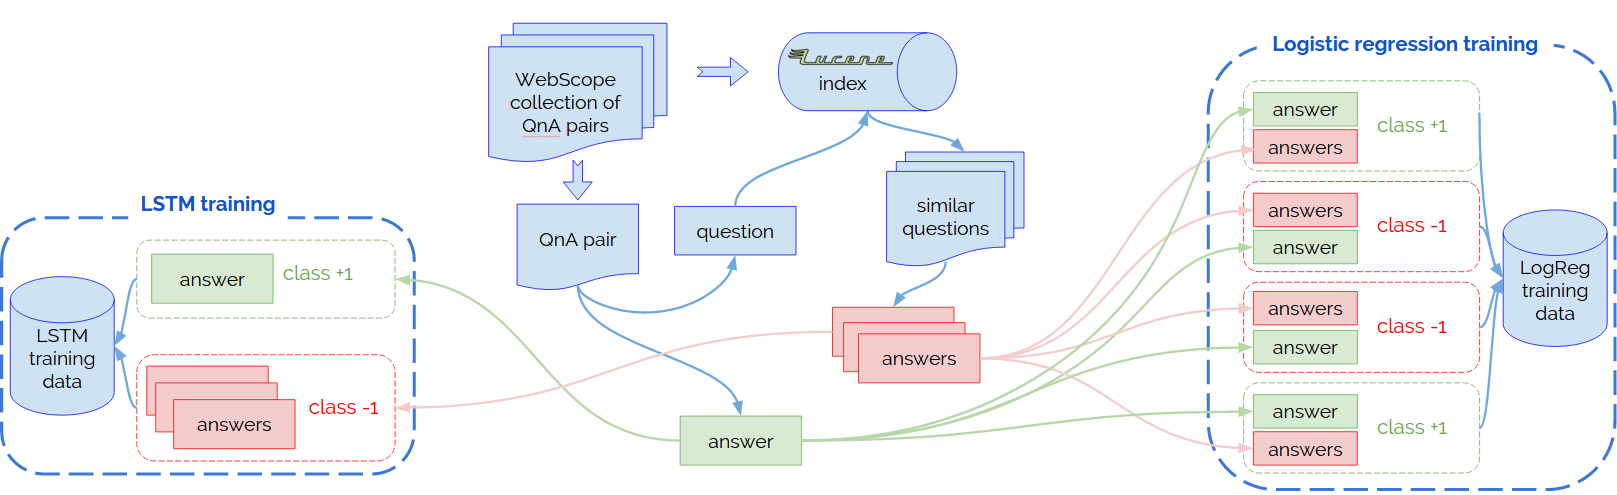
\includegraphics[width=\textwidth]{img/liveqa_model_training}
    \caption{Dataset generation workflow for training logistic regression and LSTM answer ranking models used in EmoryQA system participated in TREC LiveQA 2015.}
    \label{figure:non-factoid:system:model_training}
\end{figure}

\textbf{LSTM model}.
Deep learning models had a huge success in image and speech problems and showed very promising results in natural language processing and question answering, \eg \cite{yu2014deep,WangN15} to name a few.
Long Short-Term Memory (LSTM)~\cite{hochreiter1997long} is a particular architecture of recurrent neural networks that helps with the vanishing gradients problems.
The model reads the question and answer tokens and produces a probability score based on a vector representation of a QnA pair.
Figure~\ref{figure:non-factoid:system:lstm_model} shows the structure of the model.

\begin{figure}[t]
    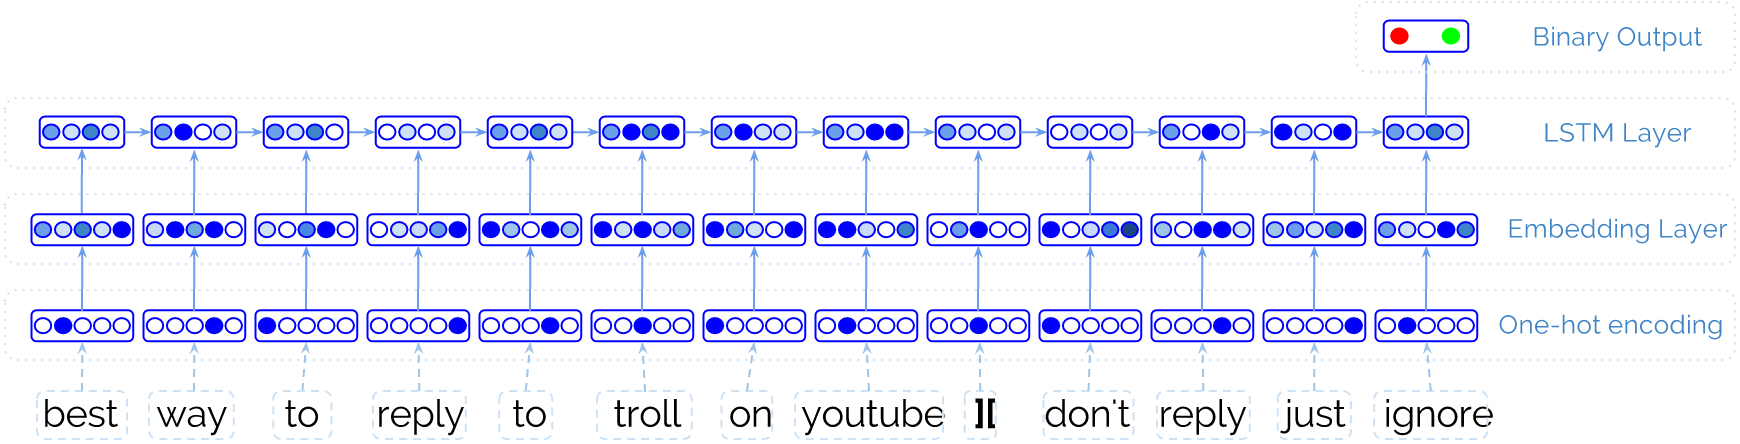
\includegraphics[width=\textwidth]{img/liveqa_qa_lstm}
    \caption{LSTM model for answer scoring used in EmoryQA system, which participated in TREC LiveQA 2015 shared task. The example shows a QnA pair where the question is ``Best way to reply to trolls on youtube?'' and the answer is ``Do not reply, just ignore''.}
    \label{figure:non-factoid:system:lstm_model}
\end{figure}

Question (title with the body) and answer texts are tokenized, punctuation characters are removed and for each token lowercased lemma is taken.
The sequences are limited to 100 elements and concatenated through a sentinel separator character so the model could learn where the question ends and the answer starts.
The hidden state of the model after the whole sequence is processed is used by logistic regression unit to output a probability, that a candidate answers the question well.

The model was trained in a pointwise learning-to-rank fashion~\cite{liu2009learning}, \ie we trained the model to distinguish between the selected best answer and some negative examples.
Random negative examples would be too unrelated to the current question, therefore I chose to use answers to similar questions only.
All QnA pairs were indexed with Lucene\footnote{\href{url}{https://lucene.apache.org/}} and similar questions were retrieved using the built-in BM25 retrieval model.
For each question and correct answer pair from the dataset 10 similar questions were retrieved and the corresponding answers were used as negative examples for training, even though some of them can indeed be relevant to the original question.

The model was implemented using the Keras\footnote{\href{url}{http://keras.io}} library.
I used an embedding and hidden layers of dimension 128 and the vocabulary size of 1M words.
The model was trained using the Adam optimization technique~\cite{kingma2014adam} with mini batches of 200 instances for 100 epochs.

\textbf{Logistic regression model}.
The final model that ranks all answer candidates is a linear L2-regularized logistic regression model.
To train the model we used a different from LSTM model split of QnA pairs from Yahoo! Answers WebScope dataset.
For each question, the corresponding ``best answer'' is taken as the correct one.
To get a sample of negative examples Lucene index is used again and answers to 10 most similar questions are retrieved.
Different from LSTM model training, here I took a pairwise approach for learning-to-rank and generated training examples from pairs of different answers to the same question, where one answer is the correct one.
That is, let the current question be $Q$, its ``correct'' answer $A^*$, and retrieved candidates $A_1, ..., A_n$.
Each candidate is represented with a set of features: $f(Q, A^*)$, $f(Q, A_1)$, ..., $f(Q, A_n)$.
For each $i=1..n$ we create two training instances, i.e. class 1: $\langle A^*, A_i\rangle$ and class -1: $\langle A_i, A^*\rangle$.
Each such instance is represented with pairwise differences of features, e.g. $\langle A^*, A_i\rangle: f_{pair}(Q, \langle A^*, A_i\rangle) = f(Q, A^*) - f(Q, A_i)$.
The trained model is linear, therefore if $w(f(Q, A^*) - f(Q, A_i)) > 0$ then $w f(Q, A^*) > w f(Q, A_i)$ and we can rank candidates by the score produced by the model, i.e. $w f(Q, A_i)$.

% ---------------------------------------
\subsubsection{Learning to rank answers with graded relevance data}
\label{table:non-factoid:system:rel_training}

The approach described in the previous section works well, but the automatic labeling introduces a certain level of noise.
When we have a set of candidate answers with specified graded relevance, as was the case for TREC LiveQA 2016, it is possible to utilize this cleaner data to train an answer ranking model.
Therefore, in TREC LiveQA 2016 for \textit{EmoryQA} we used the listwise approach to learning-to-rank and trained the LambdaMART model~\cite{burges2010ranknet}, which gave the best results on the development set.
This model was trained using the RankLib library\footnote{\href{url}{https://sourceforge.net/p/lemur/wiki/RankLib/}} on the data from the previous year TREC LiveQA task\footnote{\href{url}{https://sites.google.com/site/trecliveqa2016/liveqa-qrels-2015}}.
This data includes 1087 questions with answers provided by the participants, each of which was rated on a scale from 1(bad) to 4(excellent) by professional NIST assessors.



\subsection{Evaluation}
\label{section:non-factoid:system:evaluation}

The experimental evaluation of our \textit{EmoryQA} non-factoid question answering system was done on TREC LiveQA 2015 and 2016 tasks.
The task was to build a live question answering system to respond to user questions, which were sampled from the live stream of questions posted to the Yahoo!~Answers community question answering website by its users.
Each input question consisted of a short question title, body, and category.
A QA system had to provide an answer of 1000 characters or less within a 1 minute period using any available data source.
A reader can refer to \cite{overviewliveqa15,overviewliveqa16} for more details on TREC LiveQA 2015 and 2016 results and analysis.

During the evaluation periods, each system received 1,087 and 1,088 questions correspondingly, and responses were recorded by the organizers.
The answers to the questions were judged by the organizers on a scale:\\
\textbf{4: Excellent} - a significant amount of useful information, fully answers the question.\\
\textbf{3: Good} - partially answers the question.\\
\textbf{2: Fair} - marginally useful information.\\
\textbf{1: Bad} - contains no useful information for the question.\\
\textbf{-2} - the answer is unreadable (only 15 answers from all runs were judged as unreadable).

The official performance metrics used for the tasks are:
\begin{itemize}
\item \textbf{avg-score(0-3)}: average score over all questions, where scores are translated to 0-3 range (1 is subtracted from each judgment). This metric considers ``Bad'', unreadable answers and unanswered questions, as scored 0.
\item \textbf{succ@i+}: success at i+ metrics measures the fraction of answers with score i or greater (i=1..4).
\item \textbf{prec@i+}: precision at i+ measures the number of questions with score i or greater (i=2..4) divided by the number of answered questions.
\end{itemize}

\begin{table}[t]
\centering
\footnotesize
\begin{tabular}[t]
{p{2.5cm}|p{0.8cm}p{1.2cm}p{1.2cm}p{1.2cm}p{1.2cm}p{1.2cm}p{1.2cm}}
& avg score (0-3) & succ@2+ & succ@3+ & succ@4+ & prec@2+ &  prec@3+ & prec@4+ \\
\hline
\multicolumn{8}{c}{Results from TREC LiveQA 2016} \\
\hline
$HUMAN_{qual}$ & 1.561 & 0.655 & 0.530 & 0.375 & 0.855 & 0.692 & 0.490\\
$HUMAN_{speed}$ & 1.440 & 0.656 & 0.482 & 0.302 & 0.784 & 0.576 & 0.362\\
\hline
1. \textit{EmoryCRQA} & 1.260 & 0.620 & 0.421 & 0.220 & 0.644 & 0.438 & 0.228 \\
2. CMU OAQA & 1.155 & 0.561 & 0.395 & 0.199 & 0.596 & 0.420 & 0.212 \\
3. \textbf{EmoryQA} & 1.054 & 0.519 & 0.355 & 0.180 & 0.530 & 0.362 & 0.184 \\
\hline
Avg results & 0.643 & 0.329 & 0.212 & 0.104 & 0.422 & 0.271 & 0.131 \\
\hline
\multicolumn{8}{c}{Results from TREC LiveQA 2015} \\
\hline
1. CMUOAQA &  1.081 & 0.532 & 0.359 & 0.190 & 0.543 & 0.367 & 0.179 \\
2. ecnucs &  0.677 & 0.367 & 0.224 & 0.086 & 0.401 & 0.245 & 0.094\\
3. NUDTMDP1 &  0.670 & 0.353 & 0.210 & 0.107 & 0.369 & 0.219 & 0.111\\
\hline
\multicolumn{8}{c}{...} \\
\hline
7. \textbf{EmoryQA} & 0.608 & 0.332 & 0.190 & 0.086 & 0.408 & 0.233 & 0.106\\
\hline
Avg results & 0.467 & 0.262 & 0.146 & 0.060 & 0.284 & 0.159 & 0.065\\
\end{tabular}
\caption{Top results of the TREC LiveQA 2015 and 2016 shared tasks. EmoryQA is the described fully automatic question answering system. EmoryCRQA is a system with the integrated crowdsourcing module, described in Section~\ref{section:non-factoid:crowdsourcing}.}
\label{table:non-factoid:system:results}
\end{table}

Table~\ref{table:non-factoid:system:results} provides the results of the challenge in 2015 and 2016.
The full results can be found in the official overview reports~\cite{overviewliveqa15,overviewliveqa16}.
As we can see, \textit{EmoryQA} achieves competitive results during both 2015 and 2016 evaluation campaigns.
Improvements made in 2016, \ie additional data sources, listwise learning to rank model, trained on data from previous year task, helped to improve the average answer score by $\approx 70\%$.

Yahoo!~Answers~(qual) and Yahoo!~Answers~(speed) are answers, collected by the organizers from the original questions after a week from the postings.
The \textit{speed} answers are those submitted chronologically first, while \textit{qual} were selected as best answers by the asker, or by Yahoo's quality scoring algorithm.
As we can see, the quality of community answers are still far better, than those of QA systems.
In particular almost $\sim 50\%$ of the questions received a perfect answers from Yahoo!~Answers community, compared to $\sim 22\%$ from the winning system.
However, $\sim 20\%$ of the questions did not receive any response from the community, even though human had the whole week to respond, which stresses an importance of developing automatic approaches even more.

The distribution of answer quality scores and the difference in precision between community and QA systems show, that the later often returns an answer, which is not relevant to the question.
In addition, a quick error analysis also revealed that automatic systems often have trouble recognizing non-relevant passages, which are easily detected by a human even without domain expertise.
The next section describes \textit{EmoryCRQA}, the winning approach from TREC LiveQA 2016, which utilizes crowdsourcing inside a real-time question answering system, and significantly improves performance over the fully automatic approach.


% This plot is using my crowdsourced labels, not official, and it breaks the flow here.
% \begin{figure}
% \centering
% 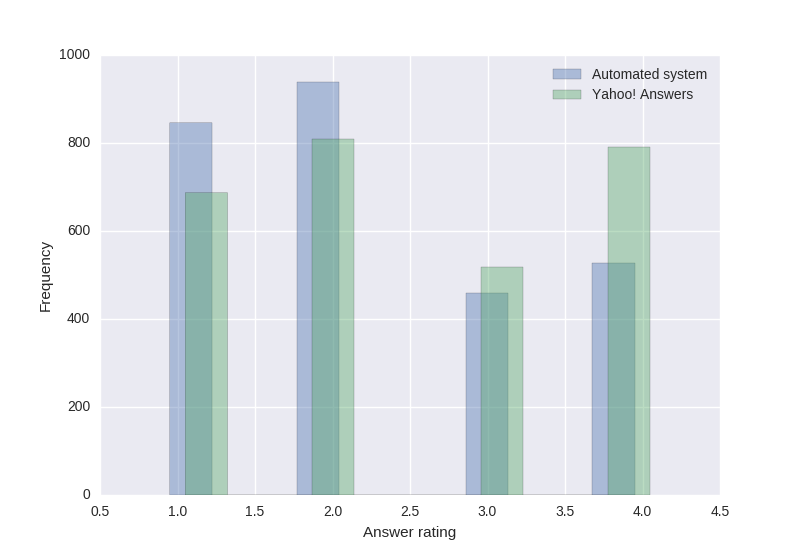
\includegraphics[width=\textwidth]{img/emoryqa_vs_yahoo_scores}
% \caption{Histogram of scores received by EmoryQA and community generated answers}
% \label{figure:non-factoid:system:emoryqa_ya_scores}
% \end{figure}

% On Figure~\ref{figure:non-factoid:system:emoryqa_ya_scores} we can see the distribution of scores received by answers retrieved by EmoryQA system and posted by the community on Yahoo! Answers.

% -=-=-=-=-=-=-=-=-=-=-=-= LiveQA : End -=-=-=-=-=-=-=-=-=-=-=-=-


% ---------------------------------------------------------------------------

\section{CRQA: Crowd-powered Real-time Automatic Question Answering System}
\label{section:non-factoid:crowdsourcing}

As we have seen in the previous section, existing question answering systems are still far from being able to handle every human question.
Answers, submitted by the community users for TREC LiveQA 2016 questions, are $\approx 35\%$ better than the answers from the best performing fully automatic system: CMU OAQA (Figure~\ref{table:non-factoid:system:results}).
One way to overcome the above-mentioned challenges in complex question answering is to develop a hybrid human-computer question answering system, which could consult a crowd of workers in order to generate a good response to the user question.
This section first describes the initial analysis of the feasibility of obtaining different types of feedback from a crowd in real-time.
Then, we present \textit{EmoryCRQA}, a crowd-powered, near real-time automated question answering system for complex informational tasks, that incorporates a crowdsourcing module for augmenting and validating the candidate answers.

More specifically, in this section we answer the following questions:
\begin{enumerate}[itemsep=0em]
\item Can crowdsourcing be used to judge the quality of answers to non-factoid questions under a time limit?
\item Is it possible to use crowdsourcing to collect answers to real user questions under a time limit?
\item How does the quality of crowdsourced answers to non-factoid questions compare to original CQA answers, and to automatic answers from TREC LiveQA systems?
\item Can crowdsourcing be used to improve the performance of a near real-time automated question answering system?
\item What is the relative contribution of candidate answer ratings and answers provided by the workers to the overall question answering performance?
\item What are the trade-offs in performance, cost, and scalability of using crowdsourcing for real-time question answering?
\end{enumerate}

Part of the described results was published at Human-Computer Question Answering workshop at NAACL 2016 conference~\cite{savenkov_crowdsourcing2016a}, and another appeared as a full paper titled ``CRQA: Crowd-powered Real-time Automated Question Answering System'' on HCOMP 2016 conference~\cite{savenkov_crqa2016}.

\subsection{Evaluating crowdsourcing for question answering}
\label{section:non-factoid:crowdsourcing:approach}

In this section I explore two ways crowdsourcing can assist a question answering system that operates in (near) real-time: by providing answer \textit{validation}, which could be used to filter or re-rank the candidate answers, and by \textit{creating} the answer candidates directly.
To test the hypothesis that crowd workers can quickly provide reliable feedback we conducted a series of crowdsourcing experiments using the Amazon Mechanical Turk platform\footnote{\href{url}{http://mturk.com}}.
We used questions from the TREC LiveQA 2015 shared task, along with the systems answers, rated by the NIST assessors\footnote{\href{url}{https://sites.google.com/site/trecliveqa2016/liveqa-qrels-2015}}.
The questions for the task were selected by the organizers from the live stream of questions posted to the Yahoo! Answers CQA platform on the day of the challenge (August 31, 2015).
For these questions, we also crawled their community answers, that were eventually posted on Yahoo!~Answers\footnote{As the answer we took the one selected as the ``Best answer'' by the author of the question or by the community.}.

\subsubsection{Answer validation experiment}
\label{section:non-factoid:crowdsourcing:approach:validation}

To check if crowdsourcing can be used to judge the quality of answers under a time limit, we asked workers to rate answers to a sample of 100 questions using the official TREC rating scale:
\begin{enumerate}[itemsep=0em]
\item Bad --- contains no useful information
\item Fair --- marginally useful information
\item Good --- partially answers the question
\item Excellent --- fully answers the question
\end{enumerate}

\begin{figure}
\centering
\begin{subfigure}[b]{0.49\textwidth}
\centering
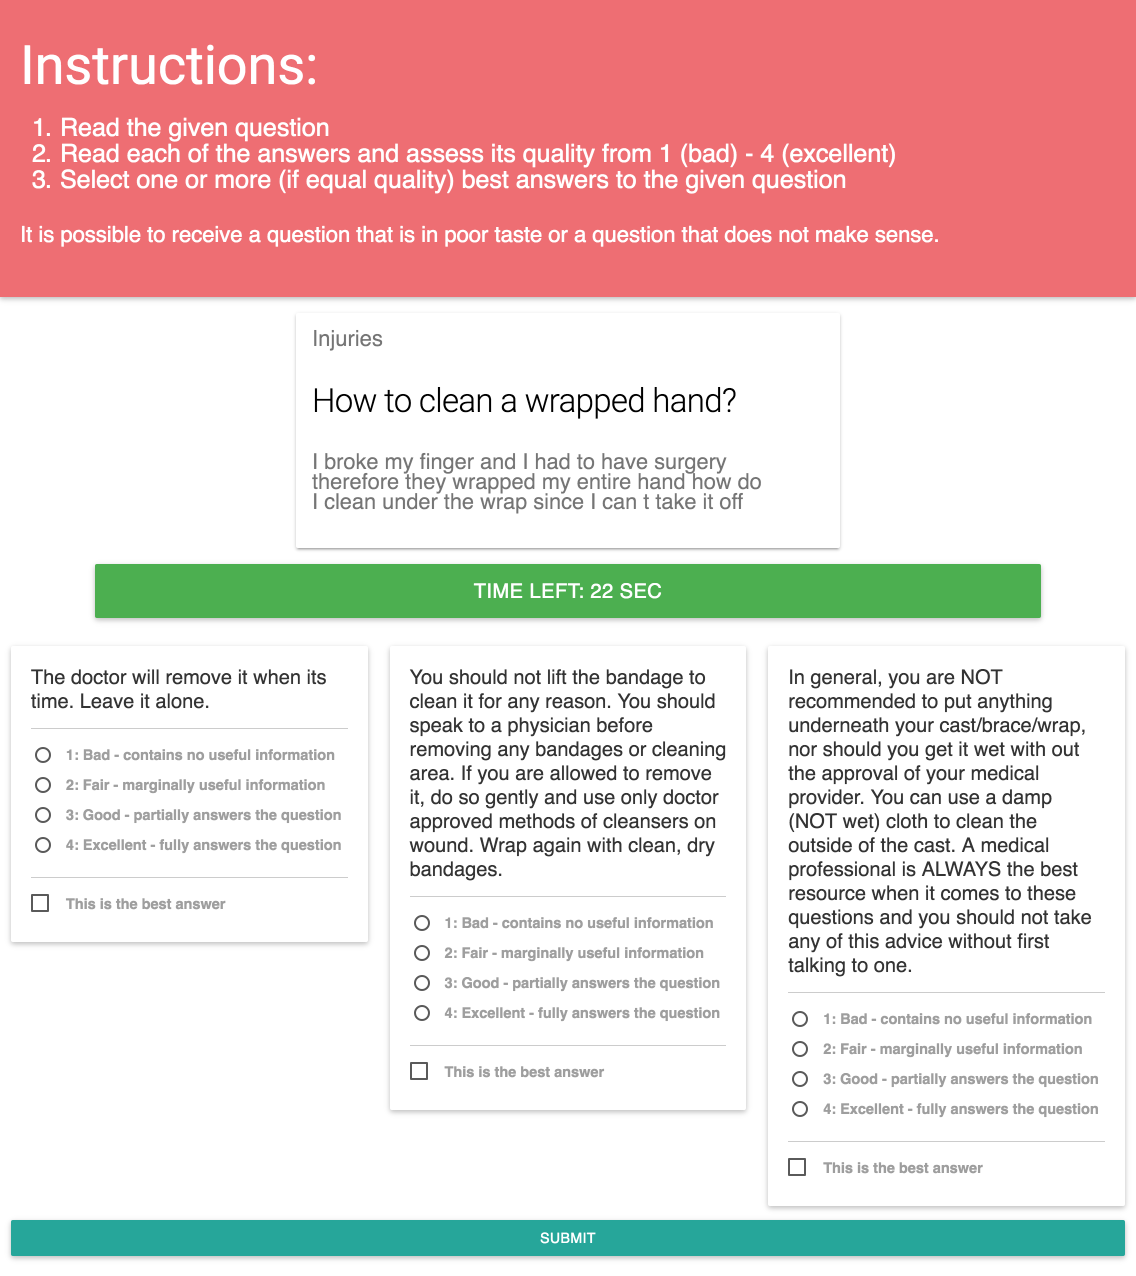
\includegraphics[width=\linewidth]{img/validation_screenshot}
\caption{Answer validation form}
\label{figure:non-factoid:crowdsourcing:interfaces:validation}
\end{subfigure}
\begin{subfigure}[b]{0.49\textwidth}
\centering
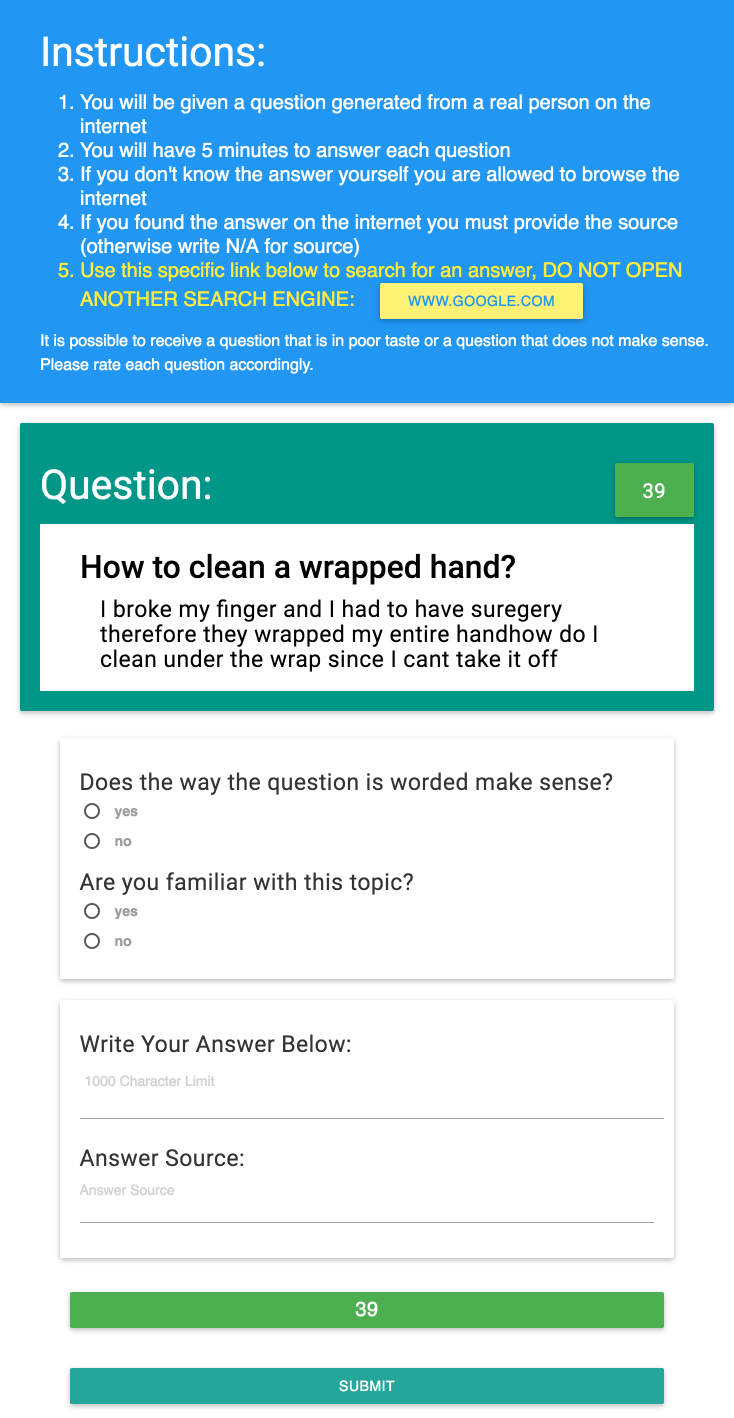
\includegraphics[width=0.9\linewidth]{img/answering_screenshot}
\caption{Answer crowdsourcing form}
\label{figure:non-factoid:crowdsourcing:interfaces:answer}
\end{subfigure}

\caption{User Interface for the answer quality judgment experiment using real-time crowdsourcing.}
\label{figure:non-factoid:crowdsourcing:interfaces}
\end{figure}

We chose to display 3 answers for a question, which were generated by three of the top-10 automatic systems from TREC LiveQA 2015 evaluation \cite{overviewliveqa15}.
To study the effect of time pressure on the quality of judgments we split participants into two groups. One group made their assessments with a 1-minute countdown timer shown to them, while the other could complete the task without worrying about a time limit.
Within each group, we assigned three different workers per question, and the workers were compensated at a rate of \$0.05 per question for this task.

The interface for collecting answer ratings is illustrated in Figure \ref{figure:non-factoid:crowdsourcing:interfaces:validation}\footnote{The screenshots show the final state of the form, as we describe later in this sections fields were unhidden step-by-step for proper timing of reading, answering and validation.}.
On top of the interface, workers were shown the instructions on the task, and question and answers were hidden at this time.
They were instructed to read the question, read the answers, and rate each answer's quality on a scale from 1 (Bad) to 4 (Excellent), and finally, choose a subset of candidates that best answer the question.
Upon clicking a button to indicate that they were done reading the instructions, the question, a 60-second countdown timer and 3 answers to the question appeared on the screen.
At the 15 second mark, the timer color changed from green to red.
In the experiments without time pressure, the timer was hidden, but we still tracked the time it took for the workers to complete the task.

At the end, we collected 6 ratings (3 with and 3 without time pressure) for each of three answers for a sample of 100 questions, which makes it a total of 1800 judgments.
Each answer also has an official NIST assessor rating on the same scale.
Figure \ref{figure:non-factoid:crowdsourcing:score_correlation} shows the correlation between official NIST assessor relevance judgments and ratings provided by our workers.
The Pearson correlation between the scores is $\rho=0.52$.
The distribution of scores shows that official assessors were very strict and assigned many extreme scores of 1 or 4, whereas mechanical turk workers preferred intermediate 2s and 3s.
The results did not show any significant differences between experiments with and without time pressure.
Figure \ref{figure:non-factoid:crowdsourcing:validation_time} shows that even though the median time to rate all three answers is around 22-25 seconds in both experiments, the upper bound is significantly lower in the experiment with the time pressure.

\begin{figure}
    \centering
    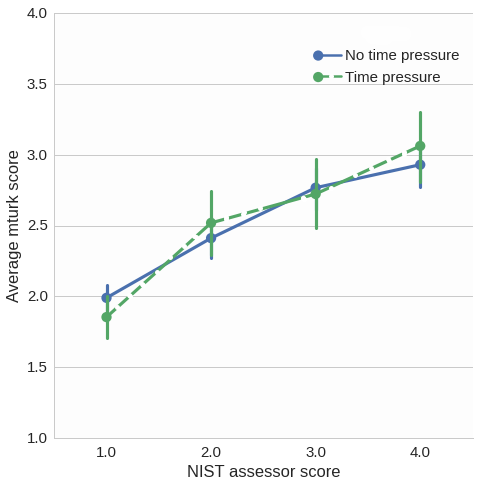
\includegraphics[width=0.5\textwidth]{img/score_correlation}
    \caption{Correlation between NIST assessor scores and crowdsourced ratings with and without time limit on the work time for answers from a sample of 100 questions from TREC LiveQA 2015 task.}
    \label{figure:non-factoid:crowdsourcing:score_correlation}
\end{figure}

\begin{figure}
    \centering
    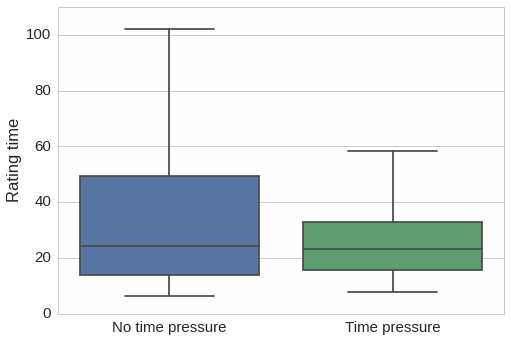
\includegraphics[width=0.5\textwidth]{img/validation_time}
    \caption{Box plot of answer rating time by workers on Amazon Mechanical Turk platform with and without time pressure.}
    \label{figure:non-factoid:crowdsourcing:validation_time}
\end{figure}

Therefore, we conclude that in general we can trust crowdsourced ratings, and on average one minute is enough to judge the quality of three answers to CQA questions.

\subsubsection{Answer generation experiment}
\label{section:non-factoid:crowdsourcing:approach:experiments:generation}

In another experiment, designed to check whether crowd workers can provide an answer to a given question within a limited amount of time, we asked different workers to answer the questions from TREC LiveQA 2015.
We split the workers into two groups and displayed a one-minute countdown timer for one of them.
We left a grace period and let the workers submit their answers after the timer had run out.
The workers received a \$0.10 compensation for each answer.
The form for answer crowdsourcing is shown in Figure \ref{figure:non-factoid:crowdsourcing:interfaces:answer}, and similar to the answer rating form, it starts with a set of instructions for the task.
We let the users browse the internet if they were not familiar with the topic or could not answer the question themselves.
To prevent them from finding the original question on Yahoo! Answers, we included a link to Google search engine with a date filter enabled\footnote{\href{url}{https://www.google.com/webhp?tbs=cdr:1,cd\_max:8/30/2015}}.
Using this link, workers could search the web as it was on 8/30/2015, before TREC LiveQA 2015 questions were posted and therefore workers were in the same conditions as automatic systems on the day of challenge\footnote{The ranking of search results could be different on the day of the challenge and for our workers}.
Initially, the question was hidden for proper accounting of question-reading and answering times.
Upon clicking a button to indicate that they were done reading the instructions, a question appeared along with a button, which needed to be clicked to indicate that they were done reading the question.
After that, the answering form appears, it contained four fields:
\begin{enumerate}[itemsep=0em]
\item Does the question make sense: ``yes'' or ``no'' to see if the question was comprehensible
\item Are you familiar with the topic: A yes or no question to evaluate whether the worker has had prior knowledge regarding the question topic
\item Answer: the field to be used for the user's answer to the given question
\item Source: the source used to find the answer: URL of a webpage or NA if the worker used his own expertise
\end{enumerate}

At the end, we collected 6 answers (3 with and without time pressure) for each of the 1087 LiveQA'15 questions.
Since we have answers from different sources, let's introduce the following notations:
\begin{itemize}[itemsep=0em]
    \item \textit{Yahoo! Answers} - answers eventually posted by users on Yahoo! Answers for the original questions
    \item \textit{Crowd} - answers collected from Mechanical Turk workers without time pressure
    \item \textit{Crowd-time} - answers collected from Mechanical Turk workers with one minute time pressure
    \item \textit{LiveQA winner} - answers from the TREC LiveQA'15 winning system
\end{itemize}

Table \ref{table:non-factoid:crowdsourcing:answer_stats} summarizes some statistics on the answers.
The first thing to notice is that, unlike CQA websites, where some questions are left unanswered, by paying the crowd workers we were able to get at least one answer for all LiveQA questions (after filtering ``No answer'' and ``I do not know'' kind of responses).
The length of the answers, provided by Mechanical turk users is lower, and time pressure forces users to be even more concise.
The majority of workers ($\sim90 \%$) did not use the web search and provided answers based on their experience, opinions and common knowledge.

\begin{table}[h]
\centering
\begin{tabular}{p{3cm}|rrrr}
Statistic & Y!A & mTurk & mTurk-time & LiveQA'15 winner\\
\hline
\% answered & 78.7\% & 100.0\% & 100.0\% & 97.8\% \\
Length (chars) & 354.96 & 190.83 & 126.65 & 790.41 \\
Length (words) & 64.54 & 34.16 & 22.82 & 137.23 \\
\end{tabular}
\caption{Statistics of different types of answers for Yahoo! Answers questions.}
\label{table:non-factoid:crowdsourcing:answer_stats}
\end{table}

\begin{figure}
    \centering
    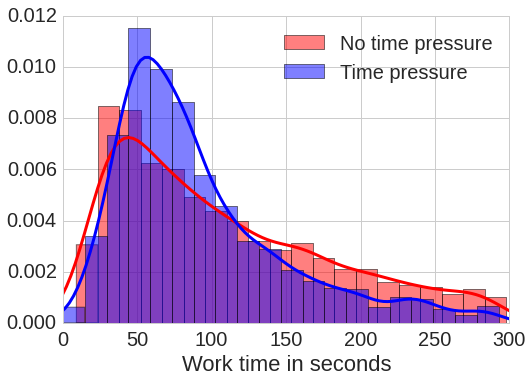
\includegraphics[width=0.6\textwidth]{img/answering_time_distribution}
    \caption{Distribution of answering times for experiments with and without time pressure.}
    \label{figure:non-factoid:crowdsourcing:answering_time_distribution}
\end{figure}

From Figure~\ref{figure:non-factoid:crowdsourcing:answering_time_distribution} we can see that adding time pressure shifts the distribution of answering times\footnote{We had separate timers for reading the instructions, the question, and writing the answer, the inclusion of instruction-reading time is why the total time could be more than 1 minute}.
The tail of longer work times for no time limit experiment becomes thin with time restrictions and the distribution peaks around one minute.

\subsubsection{Answer quality comparison}
\label{section:non-factoid:crowdsourcing:approach:experiments:comparison}

Finally, to compare the quality of the collected answers with the automatic system and CQA responses we pooled together the crowdsourced answers, the answers from the winning and \textit{EmoryQA} systems from LiveQA'15, and the original answers crawled from Yahoo! Answers.
We took a sample of 100 questions and repeated the answer rating experiment on this data.
Each answer was judged by 3 different workers (without time pressure), and their scores were averaged.
Figure~\ref{figure:non-factoid:crowdsourcing:average_score} displays the plot with average score for answers from different sources.
Quite surprisingly the quality of collected answers turned out to be comparable to those of CQA website users.
Average rating of answers produced by the winning TREC LiveQA system is also pretty close to human answers.
Finally, as expected, time pressure had its negative effect on the quality, however, it is still significantly better than the quality of \textit{EmoryQA} answers.

\begin{figure}
    \centering
    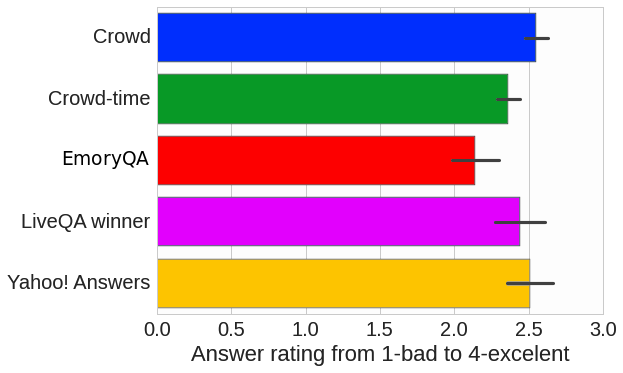
\includegraphics[width=0.6\textwidth]{img/average_score}
    \caption{Average scores of different types of answers to Yahoo! Answers questions.}
    \label{figure:non-factoid:crowdsourcing:average_score}
\end{figure}

\begin{figure}[h]
    \centering
    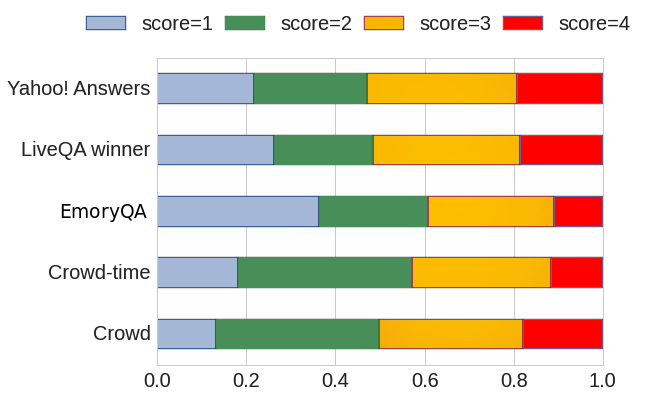
\includegraphics[width=0.6\textwidth]{img/scores_distribution}
    \caption{Distribution of scores for different types of answers to Yahoo! Answers questions.}
    \label{figure:non-factoid:crowdsourcing:scores_distribution}
\end{figure}


Analysis of the score distribution (Figure \ref{figure:non-factoid:crowdsourcing:scores_distribution}) sheds some light on the nature of the problems with automatic and human answers.
The automatic systems generate non-relevant answers ($score=1$) more often than human, either because the systems fail to retrieve relevant information or to distinguish between useful and non-useful answer candidates.
However, by having a larger information store, \eg the Web, automated QA systems can often find a perfect answer ($score=4$), while crowd workers tend to give generally useful, but less perfect responses ($score=2,3$).

Our results suggest that the ``crowd'' can quickly give a reasonable answer to most CQA questions. However, some questions require a certain expertise, which a common crowd worker might not possess.
One idea to tackle this challenge is to design a QA information support system, which a worker can use to help them find additional information.
For example, in our experiment, we let workers use a web search to find answers if they were unfamiliar with the topic; more effective search interfaces may be helpful.

\subsection{System Design}
\label{section:crowdsourcing:approach:crqa}

The findings described in the previous section were used to implement our \textit{EmoryCRQA} system (or simply CRQA), which stands for Crowd-powered Real-time Question Answering.
CRQA integrates a crowdsourcing module into an automated question answering system within an overall learning-to-rank framework for selecting answers to complex questions.
We report extensive experiments of stress-testing the CRQA system, by participating in the TREC LiveQA 2016 evaluation challenge, which provided us with a realistic evaluation setup.

\begin{figure}
    \centering
    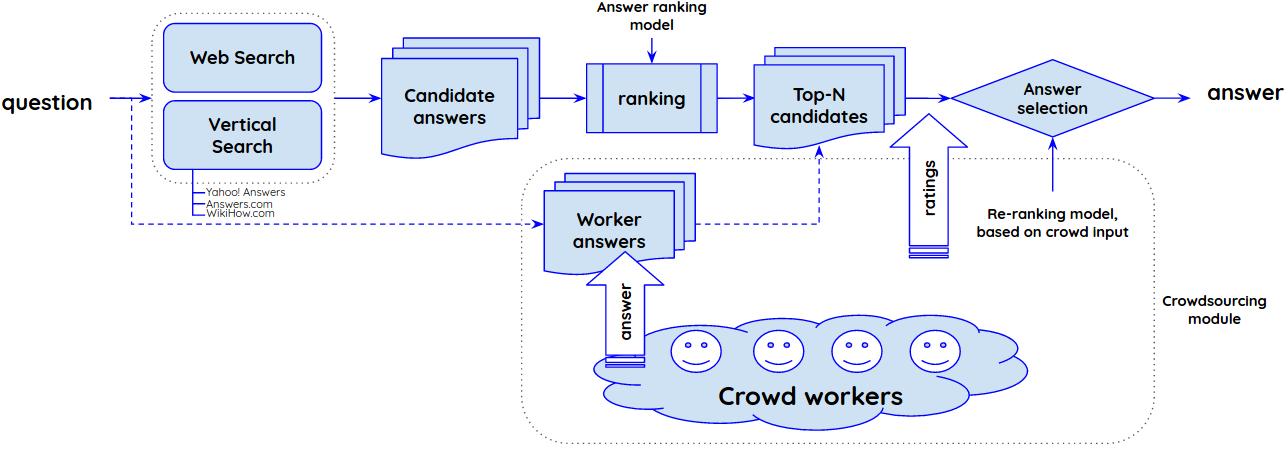
\includegraphics[width=\textwidth]{img/crqa_system}
    \caption{The architecture of our Crowd-powered Real-time Question Answering system, that uses crowdsourcing to augment a list of automatically extracted candidate answers and to rate their quality.}
    \label{figure:non-factoid:crowdsourcing:system}
\end{figure}

The high-level architecture is presented in Figure~\ref{figure:non-factoid:crowdsourcing:system}.
The automated part of the CRQA system is based on EmoryQA system, described in Section~\ref{section:non-factoid:system}.
The crowdsourcing module is designed to overcome two of the most common problems of the automated QA approaches: lack of good candidate answers and ranking errors.
More particularly, CRQA asks crowd workers to provide answers to the given questions if they can, and additionally rate the quality of candidate answers, generated by the automated system.
After the candidate answers are generated, instead of returning the final answer, as EmoryQA does, in CRQA we send the question and top-7 ranked candidates to the crowd workers and wait for the responses.
We chose to give 7 answers based on the average number of rated answers per minute in our preliminary studies.
Figure~\ref{figure:non-factoid:crowdsourcing:crowd_ui} presents the user interface of our crowdsourcing module.

\begin{figure}
    \centering
    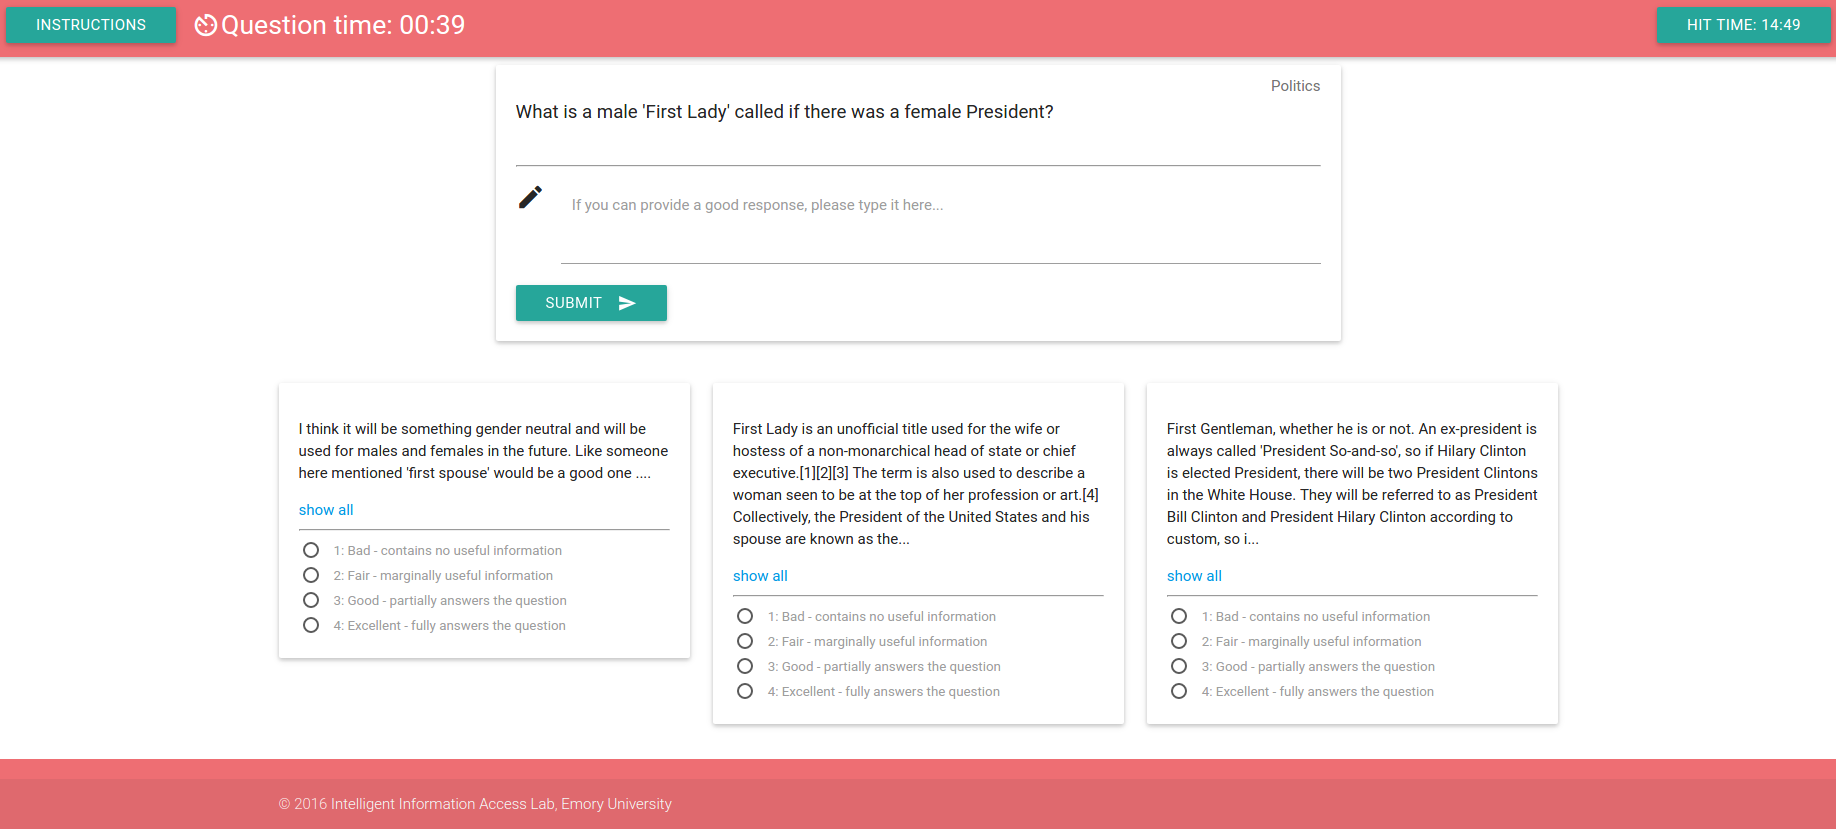
\includegraphics[width=\textwidth]{img/crqa_crowd_ui}
    \caption{User Interface for workers in our Crowd-Powered Question Answering system.}
    \label{figure:non-factoid:crowdsourcing:crowd_ui}
\end{figure}

The overall algorithm for obtaining crowd input for real-time question answering is the following:
\begin{enumerate}[itemsep=0em]
\item When the system receives a question, it is posted to the workers, who will have 50 seconds to provide their input
\item Workers are asked to write an answer if they can provide one (it is optional)
\item Otherwise they are waiting for the answer candidates to arrive
\item When the system is done with generating and ranking candidates it posts top-7 scoring answers to the workers for the rating (which usually leaves $\sim$ 35 seconds for rating)
\item Workers receive a list of answers\footnote{Answers submitted by workers are also sent for ratings to all workers except the author} and rate them until the timer runs off. Each answer is rated on a scale from 1 to 4, using the official TREC LiveQA rating scale:
    \begin{itemize}[itemsep=0em]
    \item 1 --- Bad: contains no useful information
    \item 2 --- Fair: marginally useful information
    \item 3 --- Good: partially answers the question
    \item 4 --- Excellent: fully answers the question
    \end{itemize}
\item The interface displays 3 answers at a time when an answer gets rated, it disappears and its place is taken by another answer from the pool. The interface displays only the first 300 characters of the answer, which was experimentally shown to be enough on average to make a good judgment.
Full answer can be revealed upon clicking the ``show all'' link.
\item When the timer runs off, the question and all the answers disappear, and workers wait for the next question
\end{enumerate}

To hire the workers we used Amazon Mechanical Turk platform\footnote{\href{url}{http://mturk.com}}.
Since the question answering system needs to provide a near real-time response whenever it receives a question, we adapted the ``retainer'' model for real-time crowdsourcing, inspired by the success of this model reported in previous works~\cite{bernstein2011crowds,bigham2010vizwiz}.
Specifically for TREC LiveQA 2016 task, to obtain an even distribution of workers over the 24-hour period, we posted 10 tasks every 15 minutes, and they expired after the next set of tasks became available.
Since not all assignments were accepted by some worker right away, the number of workers for each question varied and could be greater than 10.
When a worker first gets to our crowdsourcing interface, she is shown task instructions (Table~\ref{table:non-factoid:crowdsourcing:crqa:crowd_instructions}) and asked to wait for the questions to arrive.
The workers were paid \$1.00 for the whole 15 minutes task, no matter how many questions they got\footnote{In TREC LiveQA task questions are sent to the systems one by one, therefore there is no concurrency, however, the delays between the questions are possible.}.

\begin{table}[ht]
\centering
\begin{tabular}{p{13cm}}
\textbf{Instructions} \\
\hline
1. This HIT will last exactly 15 minutes\\
2. Your HIT will only be submitted after these 15 minutes\\
3. In this period of time, you will receive some questions, that came from real users on the Internet\\
4. Each question has a time limit after which it will disappear and you will need to want for the next one\\
5. If you know the answer to the question, please type it in the corresponding box\\
6. At some point, several candidate answers will appear at the bottom of the page\\
7. Please rate them on a scale from 1 (bad) to 4 (excellent)\\
8. Do not close the browser or reload the page as this will reset your assignment.\\
\end{tabular}
\caption{EmoryCRQA crowdsourcing task instructions, displayed to the user when she first gets to the task.}
\label{table:non-factoid:crowdsourcing:crqa:crowd_instructions}
\end{table}

The last stage in CRQA is answer re-ranking, which aggregates all the information received from the crowdsourcing and produces the final answer to the question.
The input of the re-ranking module is a set of candidate answers with quality ratings provided by the crowd workers.
Candidates can include the answers posted by the workers, which might also be rated if workers had enough time to do that.
To re-rank the answers we trained a gradient boosting regression trees (GBRT) model~\cite{friedman2002stochastic}.
To build this model we used a training set of questions with answers generated by our system.
The quality of each answer was manually assessed using the official LiveQA scale from 1 (bad) to 4 (excellent).
The features, used for answer re-ranking are listed in Table~\ref{table:non-factoid:crowdsourcing:crqa:reranking_features}.

\begin{table}[ht]
\centering
\begin{tabular}{p{13cm}}
\textbf{Answer-based} \\
\hline
--- The length of the answer \\
--- Source of the answer (Crowd, Web, Yahoo! Answers, Answers.com or WikiHow.com)\\
--- Original rank of the candidate answer or -1 for answers provided by the crowd workers\\
\hline
\textbf{Worker ratings} \\
\hline
--- Number of ratings provided\\
--- Minimum, maximum, median and average ratings\\
\end{tabular}
\caption{The list of features used for answer re-ranking based on crowdsourcing input in EmoryCRQA question answering system.}
\label{table:non-factoid:crowdsourcing:crqa:reranking_features}
\end{table}

CRQA sorts the candidates by the quality score predicted by the model, as returns the top candidate as the final answer.


\subsection{Experiments}
\label{section:non-factoid:crowdsourcing:experiments}

We now describe the experimental setup used to evaluate the performance of CRQA and other methods for near real-time question answering.

The experimental evaluation of our CRQA system was done on the official run of TREC LiveQA 2016 shared task, which happened on May 31, 2016.
All participating systems were running for 24 hours and received questions sampled from the live (real-time) stream of questions, posted by real users to Yahoo! Answers platform.
In total, each system received 1,088 questions, and system responses were recorded by the organizers.

\begin{table}[ht]
\centering
\begin{tabular}{r|l}
Name & Value \\
\hline
Number of questions received & 1088 \\
Number of completed assignments (15 mins each) & 889 \\
Average number of questions per assignment & 11.44 \\
Total cost per question & \$0.81 \\
Average number of answers provided by workers & 1.25 \\
Average number of ratings per answer & 6.25 \\
\end{tabular}
\caption{Aggregate statistics of the crowdsourcing tasks submitted during TREC LiveQA 2016 shared task run.}
\label{table:non-factoid:crowdsourcing:crqa:task_stats}
\end{table}

Overall statistics are provided in Table~\ref{table:non-factoid:crowdsourcing:crqa:task_stats}.
As we can see, on average workers were able to provide at least one answer for each question, and each of the provided answers got 6 ratings.

To perform a full analysis of the system, we used traditional (batch-mode) crowdsourcing to obtain the quality labels for all answer candidates that were given to the workers during the task, as well as the answers provided by the workers.
In addition, on June 2, two days after the TREC LiveQA challenge has completed, we crawled the current answers provided by the community for the questions, used for the task.
All the answers for each question were randomly shuffled and rated on a scale from 1 (bad) to 4 (excellent) by workers hired on Amazon Mechanical Turk.
As we have shown in the previous section, crowdsourced labels correlate well with the official ratings, provided by the professional NIST assessors.
Each answer was labeled by 3 different workers, and we averaged the scores to get the final quality labels for the candidates.

We compared CRQA system against several baselines:
\begin{itemize}
\item \textit{EmoryQA}: automated QA system described in Section~\ref{section:non-factoid:system}.
\item \textit{Re-ranking by score}: a simplified version of the EmoryCRQA re-ranking model, which select the answer with the highest average ratings, provided by the crowd workers.
\item \textit{Yahoo Answers}: traditional, non-real-time community question answering site (Yahoo!~Answers), from which the challenge question originated. The answers were collected two days after the challenge, thus allowing the Yahoo Answers community extra two days to collect the answers through traditional (community-based) crowdsourcing.
\end{itemize}

To evaluate the methods we used the metrics proposed by the organizers of the LiveQA task (Section~\ref{section:non-factoid:system:evaluation}).

\begin{table}[ht]
\centering
\begin{tabular}{p{4.2cm}|rrrrrr}
Method & $\overline{score}$ & $\overline{prec}$ & s@2+ & s@3+ & p@2+ & p@3+ \\
\hline
EmoryQA & 2.321 & 2.357 & 0.697 & 0.297 &  0.708 & 0.302 \\
Re-ranking by score & 2.416 & 2.421 & 0.745 & 0.319 & 0.747 & 0.320  \\
Yahoo! Answers & 2.229 & 2.503 & 0.656 & 0.375 & 0.737 & \textbf{0.421} \\
EmoryCRQA & \textbf{2.550} & \textbf{2.556} & \textbf{0.799} & \textbf{0.402} & \textbf{0.800} & 0.402 \\
\hspace{5mm}worker ratings only & 2.432 & 2.470 & 0.750 & 0.348 & 0.762 & 0.354 \\
\hspace{5mm}worker answers only & 2.459 & 2.463 & 0.759 & 0.354 & 0.760 & 0.355 \\
\end{tabular}
\caption{Evaluation of the baselines and system answers quality based on the ratings of answers obtained via crowdsourcing. The scores are averaged over 100 different 50:50 splits of 1088 questions into the training and test set. The differences between average score and precision of CRQA and the original ranking are significant at p-value $<$ 0.01.}
\label{table:non-factoid:crowdsourcing:crqa:performance}
\end{table}

Table~\ref{table:non-factoid:crowdsourcing:crqa:performance} summarizes the performance of the baselines and our system.
As we can see, the average score and precision of answers generated by CRQA system are higher than the baseline ranking and even community answers on the Yahoo! Answers platform.
However, Yahoo! Answers community answers have a higher percentage of \textit{``4 (excellent)''} scores.
Figure \ref{figure:non-factoid:crowdsourcing:crqa:score_histogram} shows the distribution of scores for the original system ranking, our crowdsourcing system and Yahoo! Answers.
Two peaks on the distribution of scores from Yahoo! Answers community suggest, that there are essentially two kinds of responses: non-useful (\eg spam) or excellent that fully answers the question.
In addition, around 20\% of the questions did not get any answer from the community.
Automatically generated answers, on the contrary, are rarely empty, but on average provide only marginally relevant information, which often does not answer the questions, and therefore rated \textit{``2 (fair)''}.
The introduction of the crowdsourcing module allowed CRQA to cover an additional couple of percents of the questions, for which the automated system was not able to generate any candidates, as well as select better candidates when it was possible using crowd ratings.

\begin{figure}[h]
    \centering
    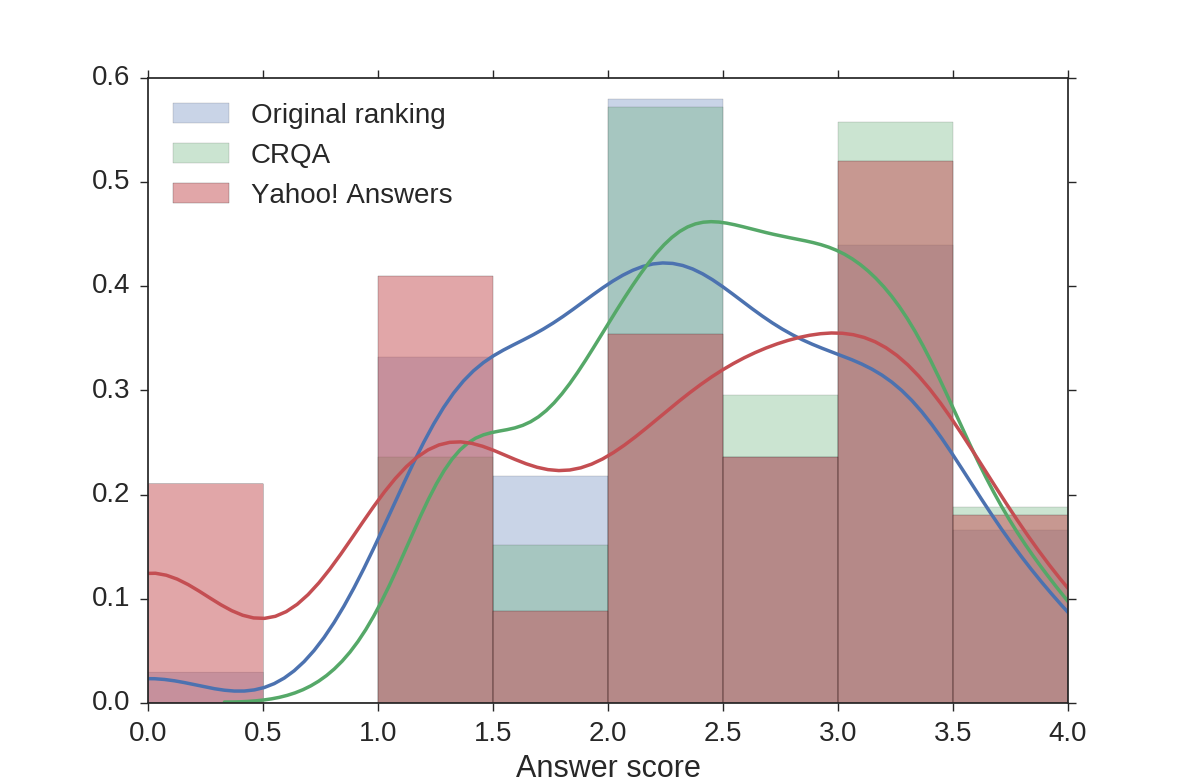
\includegraphics[width=0.75\textwidth]{img/crqa_score_hist}
    \caption{Histogram and kernel density estimation of answer scores for original candidate ranking, CPQA model re-ranking and Yahoo! Answers answers.}
    \label{figure:non-factoid:crowdsourcing:crqa:score_histogram}
\end{figure}

Even though according to the described results our system was able to achieve answer quality comparable to that of the community answers, the official results ~\cite{overviewliveqa16} give slightly different metric values, and demonstrate that there is still a big gap (Table~\ref{section:non-factoid:system:evaluation}).
However, the official scores confirm the effectiveness of crowdsourcing on top of a fully automated QA system.

\subsection{Analysis and Discussion}
\label{section:non-factoid:crowdsourcing:analysis}

In this section, we will analyze some of the results of our experiments and discuss their implications.

\textbf{Worker answers vs ratings}.
First, let's look at the contribution of additional answers and answer ratings provided by the workers.
These two types of contributions are complimentary to each other and attempt to solve different problems.
Table~\ref{table:non-factoid:crowdsourcing:crqa:performance} shows the performance of our question answering system using each of these types of feedback independently.
The results demonstrate that both answers and ratings have a positive effect on the performance.
Even with limited time, workers were able to reliably rate candidate answers, which helped the system to select a better final answer and improve the model precision.
However, this method does not help the system in cases, when it was not able to generate a good candidate in the first place, therefore using ratings only has lower average answer score than using worker generated answers.
By asking the crowd to provide a response if they can answer the question, CRQA covers this gap, which is important as in a real scenario even a fair answer would probably be better for the user than no answer at all.
Of course, given limited time and the fact that a random worker might not possess an expertise required to answer the question, such answers do not always perfectly answer the question.
Table~\ref{table:non-factoid:crowdsourcing:crqa:answer_examples} gives some examples of worker-generated answers with low and high-quality scores.

% To summarize, ratings of answer candidates and worker generated answers both have a similar positive effect on the performance of our question answering system.
% What is more important, the contributions are independent and therefore it is beneficial to use both of them in the final system.

\begin{table}
\centering
\small
\begin{tabular}{p{6cm}|p{5cm}|l}
Question & Answer & Score \\
\hline
 Is Gotu Kola a good herb for mental health? How long does it take to work?? & yes & 1.66\\
 \hline
Can I write any number on line number 5 of a W2?  would like to set up my W2 were I get the most out of my paycheck... & W2 & 1.33\\
 \hline
...i randomly asked my mother why when I lived with you in your home country a man that was our neighbour used to call me his daughter...? & yes & 1.0\\
\hline
\hline
 Is it bad not wanting to visit your family? & It is nt bad. Just be honest with them. They may be upset but they should understand & 3.0 \\
 \hline
Any health concerns with whey protein?... & As long as you use it as directed, there should not be any major problems.  You may want to consult your doctor just in case. & 3.0\\
\hline
Foot pain unable to walk? Hi so today woke with some pain, I am able to put weight on my heel with no problem or pain... & Possible gout in your foot, also possible you may have strained it during the previous day. & 3.0\\
\hline
What is a good remedy/medicine for stomach aches? Specifically ones caused by stress or anxiety? & Chamomile tea should help & 3.66\\
\end{tabular}
\caption{Examples of questions, answers and their quality scores, provided by the crowd workers during TREC LiveQA 2016 shared task.}
\label{table:non-factoid:crowdsourcing:crqa:answer_examples}
\end{table}

\textbf{Selection of answer candidate for rating}.
We have seen that crowd workers are able to provide reliable answer ratings, which can be used to re-rank them and select a better final response.
However, since a system usual has hundreds or thousands of candidate passages, the capacity of crowdsourcing is limited.
We chose to show top-7 answers according to the trained learning-to-rank model, however, the order in which the answers are shown can also have a strong effect on the system performance, because the answers are typically rated one by one in the order they are displayed on the screen.
Our system included two strategies for answer ordering: random or according to their ranking score.
The former strategy provides a uniform coverage for all the answers selected for rating, while the later puts more emphasis on the currently top scoring candidates.
We randomly selected one of the strategies for each user and question.
To analyze the performance of each of the strategies we compute the average score of answers, generated using the corresponding ratings.
The average score for answers generating when candidates are shuffled is 2.508, and it is 2.539 when the candidates are sorted according to their model ranking score.
This suggests, that it is beneficial to allocate more of the worker's attention on the top scoring candidate answers.

\textbf{Cost analysis}.
The results of our experiments clearly demonstrated that crowdsourcing can improve the performance of near real-time question answering system.
The next reasonable question is what is the price of this improvement.
In our study, we paid workers \$1.00 per single 15 minutes task, and each 15 minutes we had 10 assignments, which translates to \$15.00 per 15 minutes.
Overall, our experiment cost \$0.88 per question, and in this section, we will discuss some ideas to reduce this cost.

First, we will study the effect of the number of workers on the performance of our CRQA system.
For this experiment, we randomly sampled a certain percentage of workers and removed all contributions (answers and ratings) of others.
Figure~\ref{figure:non-factoid:crowdsourcing:crqa:nworkers_vs_quality} plots the dependency of the performance of our QA system on the number of workers.

\begin{figure}
  \begin{subfigure}[t]{0.5\textwidth}
    \centering
    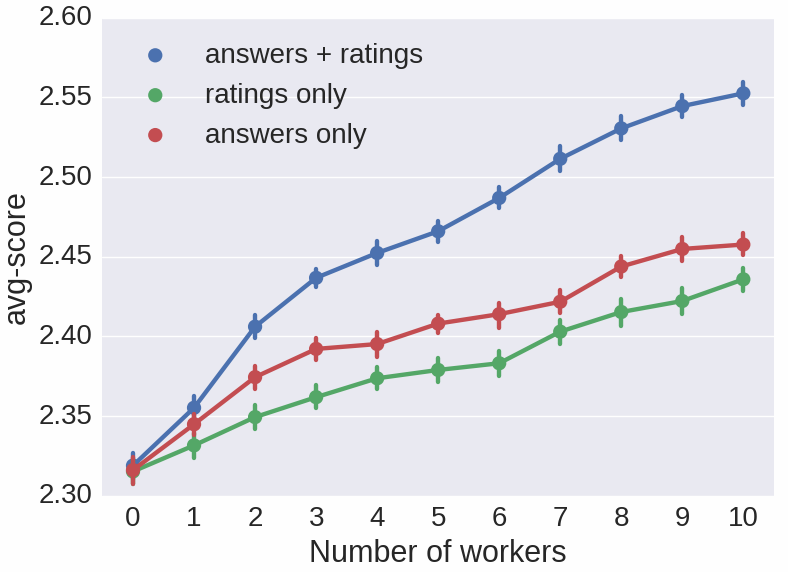
\includegraphics[width=\textwidth]{img/crqa_nworkers_vs_accuracy}
    \caption{avg-score: Average score per question}
    \label{figure:crqa:nworkers_vs_accuracy}
  \end{subfigure}
  \begin{subfigure}[t]{0.5\textwidth}
    \centering
    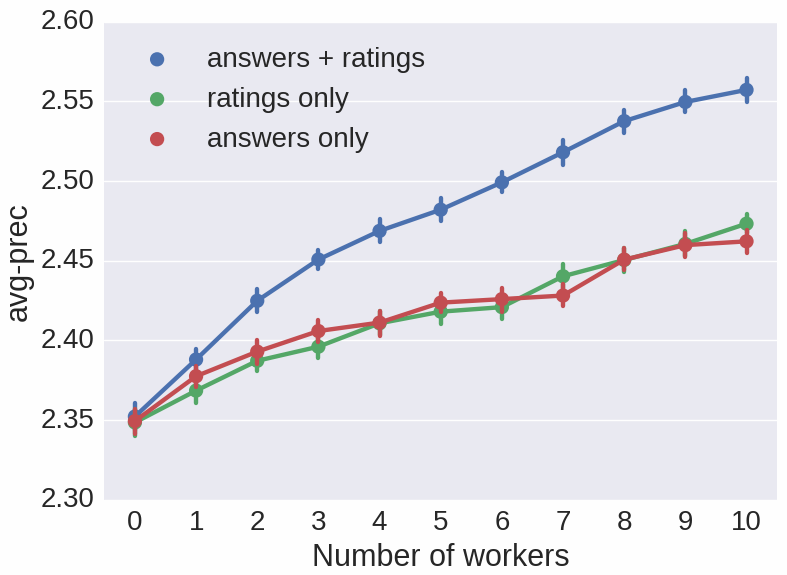
\includegraphics[width=\textwidth]{img/crqa_nworkers_vs_precision}
    \caption{avg-prec: Average score per answer (ignoring non-answered questions)}
    \label{figure:crqa:nworkers_vs_precision}
  \end{subfigure}
    \caption{Plot showing how the quality of the final answer depends on the number of workers per question}
    \label{figure:non-factoid:crowdsourcing:crqa:nworkers_vs_quality}
\end{figure}

Obviously, more workers mean more reliable answer ratings and more answer candidates, which improves the performance of the question answering system.
However, we can observe diminishing returns: the cost per extra gain in performance metrics decreases as the number of workers grows.
Half of the overall performance improvement could be achieved with only 3 workers per question, which would save 70\% of the costs.

An alternative cost-reduction strategy is selective triggering of crowdsourcing, which would only ask for workers feedback for some of the questions.
Such a strategy would be necessary to scale a crowd-powered question answering system to a higher volume of questions.
There are multiple different approaches for such selective crowdsourcing: \eg a system can only ask for crowd contributions if it did not generate enough candidate answers or the predicted quality of the top scoring candidates is low~\cite{carmel2010estimating,he2006query}.
We leave this questions for the future work, as here we focused on the scenario, proposed by the organizers of the TREC LiveQA shared tasks, where questions arrive one by one and it is possible to utilize crowd input for every question.

To summarize, in the explored real-time QA scenario it is possible to reduce the costs of crowdsourcing by reducing the number of workers, although with some performance losses.
Our analysis suggests that paying 30\% of the original cost would give 50\% of the performance improvement.

% The described CRQA implementation is a promising step towards the efficient and close integration of crowd work and automated analysis for real-time question answering.
% It raises many promising issues and opens directions for future work, such as selective crowdsourcing for only the questions deemed ``difficult'' for the automated system; more efficient online learning for obtaining ratings from the crowd and integrating them into the ranking model; and investigating additional features and sources of evidence for improving the joint ranking of the system and crowd input.

\section{Summary}
\label{section:non-factoid:summary}

This chapter described two QA systems aimed at answering a general class of user information needs, often referred to as non-factoid questions.
A fully automatic \textit{EmoryQA} system has information retrieval techniques at its basis, \ie it extracts relevant passages from multiple semi-structured and unstructured sources, represents them with a set of features, uses a learning-to-rank model to sort the candidate answers and selects the top one as the final answer.
The system was experimentally tested on TREC LiveQA 2015 and 2016 shared tasks, achieving very competitive results.
The source code of the system is available at \href{url}{https://github.com/emory-irlab/liveqa}.

The analysis of the TREC LiveQA results revealed that automatic systems often have problems distinguishing between information, that is totally irrelevant and something, that might be of potential use to a user.
As a result, compared to community generated responses, automatic QA systems have a higher fraction of answers, rated ``bad''.
Many of these mistakes can easily be spotted by a human, even without a specific domain expertise.
\textit{EmoryCRQA} extends the fully automatic QA system with a crowdsourcing module, which obtains feedback from a crowd of workers in a form of additional answer candidates and ratings of existing passages, while still operating in near real-time.
Results of TREC LiveQA 2016 task confirmed the effectiveness of crowdsourcing in this scenario.
The analysis presented in Section~\ref{section:non-factoid:crowdsourcing:analysis} shows that both worker contributed answers and ratings make an equal impact on the overall answer quality.
The described CRQA implementation is a promising step towards the efficient and close integration of crowd work and automatic analysis for real-time question answering.

These contributions have laid the groundwork for future research in non-factoid question answering, using various types of semi-structured (QnA pairs), unstructured (web documents) and real-time crowdsourcing data.
Together, the proposed methods enabled substantial performance improvements in answering a wider class of user information needs.		\clearpage
\chapter{Conversational Question Answering}
\label{chapter:conversation}

Chapters~\ref{chapter:factoid} and~\ref{chapter:non-factoid} focused on improving the answer retrieval performance for different types of user information needs.
However, question answering is not a one-way communication, where a user is only responsible for issuing requests and a system has to generate answers.
This setup is quite limited because it does not provide any means for the user to affect the behavior of a question answering system except by issuing new questions.
Similarly, it does not allow QA systems to request any additional information from the user, nor learn from the previous interactions.

Proliferation of mobile devices and more ``natural'' interfaces~\cite{hearst2011} are changing the way people search for information on the web.
Many experts envision that search in the near future will be a dialog between a user and an intelligent assistant, rather than just ``ten blue links'' in response to a one-shot keyword query.\footnote{\url{http://time.com/google-now/}} 
Participants of the SWIRL'2012 workshop foresaw a fusion of traditional IR and dialog systems~\cite{swirl2012}: ``Dialogue would be initiated by the searcher and proactively by the system.
The dialogue would be about questions and answers, with the aim of refining the understanding of questions and improving the quality of answers.''
Today we can witness this trend embodied in such products as Amazon Alexa, Google Home, Microsoft Cortana, Apple Siri, and others.

This chapter presents the research towards designing better conversational search interfaces.
Section~\ref{section:conversation:user-study} describes the user study we performed to learn how people use dialogs for information seeking scenarios and how the experience with modern personal assistants compares to a human-to-human dialog.
Sections~\ref{section:conversation:hints} and~\ref{section:conversation:clarq} focus on two particular interaction strategies, which allows a QA system to help the user either formulate or clarify their questions.

The contributions of the research described in this chapter are:
\begin{itemize}
\item A user study on conversational search, which provides actionable feedback on what people expect from such systems, how the expectations towards an automatic system differ from those towards humans, and what are some of the problems with using existing commercial personal assistants.
This work will be presented at CHI 2017 conference~\cite{vtyurina2017convsearch}.
\item A study of the effect of strategic hints, that a system might provide to the user, on search experience and success rate for complex informational tasks.
This work has been published as a short paper at SIGIR 2014~\cite{savenkov2014hint}.
\item An extensive analysis of clarification questions on community question answering platforms, and a model to predict the subject of a popular type of clarification questions, which shows the potential of such an approach.
This results were published in CHIIR 2017 conference proceedings~\cite{braslavski2017clarq}.
\end{itemize}

% =============================== User Study ===========================
\section{Conversational Search With Humans, Wizards, and Chatbots}
\label{section:conversation:user-study}

Chatbots and conversational assistants are becoming increasingly popular.
However, for information seeking scenarios, these systems still have very limited conversational abilities, and primarily serve as proxies to existing web search engines.
In this section, we ask: what would conversational search look like with a truly intelligent assistant?
To begin answering this question empirically, we conduct a user study, in which 21 participants are each given 3 information seeking tasks to solve using a text-based chat interface.
To complete each task, participants conversed with three conversational agents: an existing commercial system, a human expert, and a \textit{perceived} experimental automatic system, backed by a human ``wizard'' behind the curtain.
The observations and insights of our study help us understand the aspirations of users and the limitations of the current conversational agents -- and to sharpen a frontier of work required to improve conversational assistants for search scenarios.

\subsection{Motivation}
\label{section:conversation:user-study:motivation}

Personal assistants, such as Amazon's Alexa, Google Home, \etc are becoming increasingly popular, and people are integrating them in everyday life, \eg for simple tasks like setting up a timer, checking the calendar, requesting the latest news, a song, etc.\footnote{\href{url}{https://arc.applause.com/2016/09/26/amazon-echo-alexa-use-cases/}}.
The popularity of text-based chatbots is also on the rise in many areas of the web~\cite{ferrara2014rise}.
Most of them are template-based and are designed to fulfill a single, often monotonous, job~\cite{clement2015interacting,edwards2014bot}.
At the same time, a growing proportion of web search queries is formulated as natural language questions~\cite{aula2010does,liu2012web,pang2011search}, which is partially explained by the increasing usage of voice interfaces~\cite{white2015questions}.
Alas, for information seeking scenarios, existing chatbots and intelligent assistants are usually implemented as simply a ``proxy'' to existing web search engines, even though question-answering technology has made dramatic progress handling such question-like queries~\cite{tsai2015web}.
Furthermore, conversation provides additional opportunities to improve search quality. For example, a conversational system should be able to ask clarification questions~\cite{braslavski2017clarq} to better identify searcher's intent, and incorporate explicit user feedback~\cite{radlinski2017} -- something that is not normally available in a traditional web search scenario.
However, before jumping into implementing additional features for conversational search systems, it is important to gain a better understanding what the users' expectations are when interacting with a truly intelligent conversational search agent. It is equally important to anticipate how users might behave when faced with a conversational search system since behavioral feedback is critical for system evaluation and improvements. To this end, we explore the following research questions:

\begin{itemize}[noitemsep]
\item \textbf{RQ1}: What are the main expectations from a conversational search system?
\item \textbf{RQ2}: What are the differences between human-to-human and human-to-computer conversations?
\item \textbf{RQ3}: What characteristics prevent existing conversational agents from becoming effective tools for complex information seeking?
\end{itemize}

As no truly intelligent conversational search systems exist yet, we explore these research questions with a mixture of survey methods and user studies.
In the user study, the participants are faced with 3 complex information search tasks, derived from TREC Session track tasks~\cite{sessionTrack2014Overview}.
To eliminate the voice recognition quality variable, we chose to use text messaging as the interface between a participant and conversational systems.
We use three different conversational systems answering user requests: an existing commercial intelligent assistant, a human expert and a human disguised as an automatic system.
The results of our exploration suggest:
(1) people do not have biases against automatic conversational systems, as long as their performance is acceptable;
(2) existing conversational assistants are not yet up to the task, \ie they cannot be effectively used for complex information search tasks;
(3) by addressing a few requests from users that we identified, even current search systems might be able to improve their effectiveness and usability, with feasible modifications. 

\subsection{Study design}
\label{section:conversation:user-study:design}

\begin{figure}[h!]
	\centering
	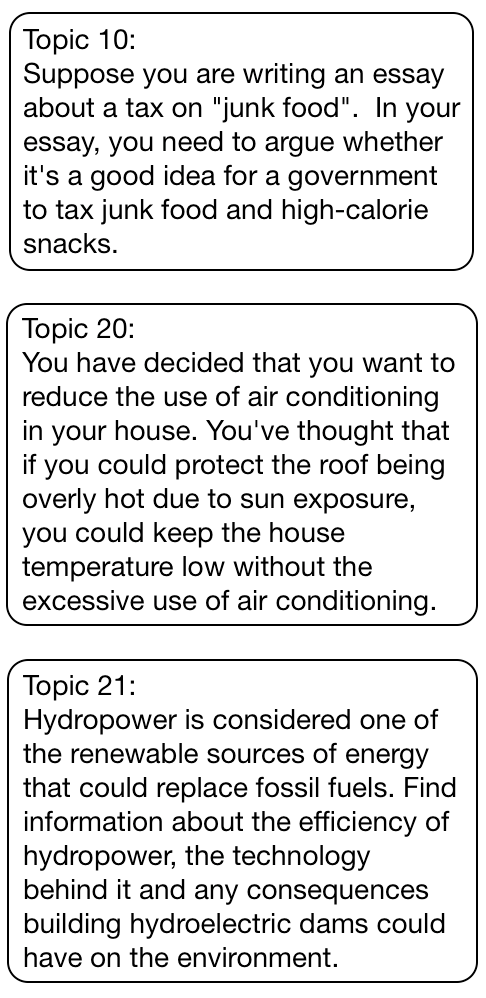
\includegraphics[width=0.4\textwidth]{img/FramedTopicsLeftAlign}
	\caption{Description of the tasks used in the user study on conversational search. All the tasks were obtained from TREC Session track 2014~\cite{sessionTrack2014Overview}.}
	\label{figure:conversation:user-study:tasks}
\end{figure}

We recruited 21 participants (graduate and undergraduate students at Emory University), to complete 3 different complex search tasks, taken from the TREC Session track 2014~\cite{sessionTrack2014Overview} (Figure~\ref{figure:conversation:user-study:tasks}).
The participants were asked to use an assigned text messenger-based conversational agent.
They were not given any instructions on how to use the agent and therefore were free to interact with it in any way they chose.
They were allowed to spend up to 10 minutes working on each task, after which they were asked to move on a topical quiz, consisting of 3 questions, designed for the topic.
After seeing the topical quiz questions, the participants were not allowed to talk to the agent anymore.
By doing so we ensured that the task stayed exploratory in nature, \ie the participants did not have a set of predefined points to cover.
After completing a topical quiz, the participants filled out a preference questionnaire, where they were asked to rate their experience with the agent, provide feedback about advantages and disadvantages of the agent.
After completing all tasks they filled out a final questionnaire.
The communication was implemented through the Facebook Messenger interface\footnote{\href{url}{http://www.messenger.com}}.
Participants used a Facebook account created specifically for the purpose of the study.
Message history was cleared prior to every experiment.

\subsubsection{Wizard agent}
\label{section:conversation:user-study:design:wizard}
Our first research question explores human behavior in human-computer communication.
There are currently no general purpose intelligent conversational search systems, that we could use for our purposes.
Therefore we ``faked'' one by substituting the backend with a person.
However, the participants were told that it was an experimental \textit{automatic} system, thus following a general Wizard-of-Oz setup.
We will be further referring to this system as the Wizard agent, and the person in the backend as the Wizard.
The Wizard had done the research about the topics of the 3 tasks prior to the experiment and compiled a broad set of passages covering most of the aspects of each topic.
At the time of the experiment, the Wizard tried to find the best passage to reply to the participant's question/comment.
However, in cases where such passage could not be found, the Wizard would reply with a passage retrieved from web search, or write a new passage.
In case the participant's question or comment was ambiguous, the Wizard was allowed to ask a clarification question to better identify the information need of the participant.
Our Wizard agent was allowed to maintain the context of the conversation, respond to vague questions, understand implied concepts, and provide active feedback in form of clarification questions when needed (all of these capabilities do not yet exist in commercial systems).
At the same time, by partially restricting the Wizard to a pre-compiled set of passages, we could maintain some consistency of answers between participants, \ie for the same question any participant would receive the same answer.
By analyzing the ways the participants communicated with the Wizard agent, we could gain insights about strategies people use in a human-computer dialogue for solving complex tasks and look for design implications for automatic conversational systems.

\subsubsection{Human agent}
\label{section:conversation:user-study:design:human}
To answer our second research question, about the differences between human-to-human and human-to-computer communication, we devised our second conversational agent -- the Human agent.
In this case, the Wizard from the previous setup was still serving as a backend, but the participants were explicitly informed that they were talking to a live person.
Another difference was that the Human agent was restricted to the pre-retrieved set of passages, but was free to slightly reformulate or revise the passages to better respond to the question.
By including both the Human and Wizard agents in the study, we were able to maintain a constant level of intelligence for both agents, thus comparing not the accuracy of each agent, but rather the participants' attitude and expectations towards a perceived automatic agent compared to a known human.

\subsubsection{Automatic agent}
\label{section:conversation:user-study:design:google}
For a comparison with an existing conversational agent, we used the Google Assistant\footnote{\href{url}{https://assistant.google.com/}} as a backend for our third agent.
Every message sent by a participant was forwarded to the Google Assistant app, and the response was forwarded back to the participant.
Most of the time, the response consisted of an URL and a text snippet. The participants were told that they were interacting with another experimental conversational system, but were not given any specific information about it.
By using a system representative of the state-of-the-art technology, we were able to evaluate its drawbacks, and situations where it failed to respond properly.

\subsection{Results}
\label{section:conversation:user-study:results}

After running the study, we analyzed message logs, answers to topical quizzes, and preference questionnaires and found the most popular trends and answers.
This section describes our findings in detail.
\begin{table}
  \centering
    \begin{tabular}{l*{4}{c}r}
    Agent                      & Human & Wizard & Automatic \\ 
    \hline
    Overall satisfaction       & 4.1 & 3.8 & 2.9 \\ 
    Able to find information   & 1.5 & 1.3 & 1.0 \\ 
    Topical quiz success       & 1.6 & 1.6 & 1.3 \\
    \end{tabular}
  \caption{Statistics on user satisfaction and success rates with human, wizard and automatic agent in conversational search user study.}
  \label{table:conversation:user-study:results}
\end{table}

\subsubsection{Overall satisfaction}
After completing each task participants rated their overall experience of working with each agent on a 1 to 5 Likert scale.
Average ratings for each agent are shown in Table~\ref{table:conversation:user-study:results}.
The differences in ratings of Human vs. Automatic systems, and the Wizard vs. Automatic systems were statistically significant (p $<$ 0.0001 and p $<$ 0.0005 respectively), while the difference between the Human vs. Wizard systems was not significant.
In the final questionnaire, after completing all the tasks, participants were asked which system they liked the most.
Out of 21 people, 8 people preferred the Human agent, 6 -- the Wizard agent, 4 -- the Automatic agent, 2 people said they would use the Wizard or the Human depending on their goals, and 1 person said he would choose between the Human and the Automatic agent depending on her goals.

\subsubsection{Able to find information}
Participants were asked whether they were able to find all the information about the topic they were looking for.
We coded each answer on a 0-2 scale (0 - no, I couldn't; 1 - partially; 2 - yes, I found everything I needed).
Average results for each agent are shown in Table~\ref{table:conversation:user-study:results}.

\subsubsection{Topical quiz success}
After completing each task participants were also asked 3 questions about the topic. We evaluated those questions on a scale 0-2, where 0 meant no answer, 1 - poor answer, 2 - good answer.
On average, participants showed a similar level of success with each agent.
The average user ratings for each agent are shown in Table~\ref{table:conversation:user-study:results}.

These results confirm our initial intuition that human-to-human conversation is more natural for the open-ended problem of the complex search task, compared with automatic conversational agents. This could be because people have experience talking to other people, and the results match their initial expectations. On the other hand, for any system that people have no experience with, they have to learn its functionality and ways to interact with it effectively.

We now turn to qualitative results, reporting the comments participants provided in the post-study questionnaire. The participants' comments broke down into the areas of maintaining context, trustworthiness, and social burden.

\subsubsection{Maintaining context}

\begin{figure}
    \centering
    
\includegraphics[width=0.5\textwidth]{img/conversation_userstudy_context}
    \caption{Automatic system (gray background) fails to maintain context, which causes the participant 15 (blue background) to reformulate his question twice.}
    \label{figure:conversation:user-study:context}
\end{figure}

\textit{Participant 19 (P19): ``It didn't use contextual information so there was no way to expand on the previous answer it gave me.''} Within a conversation, people expect that the main topic of the discussion is maintained, and they tend to ask short questions, omitting the subject, or referring to the subject using pronouns. Formulating a full question takes effort and is unnatural. For the Automatic system, anaphora resolution did not always work, which annoyed the participants. Similarly, when dealing with the Human and Wizard systems, participants pointed out the ease of use, because their partially stated questions were understood, and relevant answers were returned (Figure~\ref{figure:conversation:user-study:context}).

\subsubsection{Trustworthiness of the sources is crucial}

\begin{figure}
    \centering
    
\includegraphics[width=0.5\textwidth]{img/conversation_userstudy_prefersearch}
    \caption{A participant prefers web search to talking to a person. Part of a conversation between participant 7 (blue background) and Human agent (gray background).}
    \label{figure:conversation:user-study:prefersWebSearch}
\end{figure}

\textit{P7: ``I ... like to be able to verify the credibility of the sources used.''} Even though the Automatic system did not always respond with a relevant result, it received approval from our participants for providing sources of its answers. Out of 21 participants, 13 people said that being able to access the URL allowed them to assess the trustworthiness of the source and therefore to accept or reject the answer. On the other hand, in spite the Human and Wizard systems returning more relevant results, they were both criticized for not providing the sources (Figure~\ref{figure:conversation:user-study:prefersWebSearch}).

\subsubsection{Social burden}

\begin{figure}
    \centering
    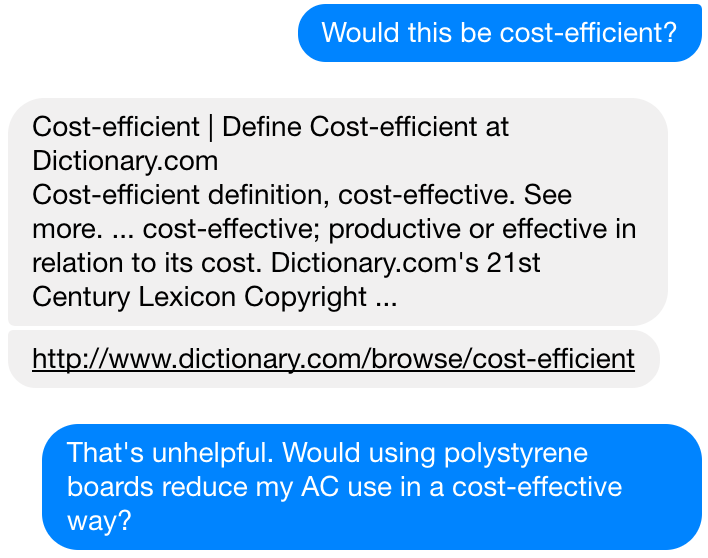
\includegraphics[width=0.5\textwidth]{img/FullExample1}
    \caption{Explicit user feedback could be used to recover from failure. Part of a conversation between participant 12 (blue background) and Automatic system (gray background).}
    \label{figure:conversation:user-study:feedback}
\end{figure}

\textit{P15: ``you have to think about social norms, asking too much, being too stupid, not giving them enough time to respond, troubling them.''} When dealing with the Human system, 4/22 participants reported that they felt uncomfortable talking to a person, thought more about the social norms, were afraid to ask too many questions, were not sure how to start and end a conversation. This additional burden of interacting with humans further motivates research in the area of automated conversational agents as the medium of choice for a notable fraction of use cases (Figure~\ref{figure:conversation:user-study:feedback}).


\subsection{Discussion and design implications}
\label{section:conversation:user-study:discussion}

Based on our findings we devised a list of recommendations for a conversational agent design, that according to our empirical study will improve user experience significantly.

\textbf{Context.}
Maintaining a context of the conversation to enable short questions and comments is crucial to user experience since formulating long sentences each time feels unnatural and takes longer.

\textbf{Provide sources of answers.}
Finding relevant and precise answers is important. But trustworthy sources are equally important, and their absence may diminish the credibility of the system. While the Automatic agent supported each answer with an URL, Human and Wizard did not, unless specifically asked. 
%This may have impacted the user satisfaction with the system, confirmed by anecdotal feedback from the participants.

\textbf{Use feedback.}
One crucial difference of conversational setup from web search is the ability of a user to provide the system with explicit feedback. It is likely to contain essential information that may help the system to get back up from failure and improve upon the previous result. 
%Feedback processing may also be of help in case a user decides to switch the focus of the search. It will also produce rich data for user satisfaction evaluation. \\

\textbf{Opinion aggregation.}
According to the participants, sometimes what is needed is the \textit{experience} of other people in similar situations.
A good conversational system should be able to aggregate opinions and present them to the user in a short summary, perhaps explaining each one. 
Participant 17 said: \textit{``It would be nice if I could see a summarization of different opinions that there exist -- from different sources.''}
% This is why they may prefer to talk to a friend -- to learn about the experiences of a knowledgeable trustworthy person or to get a broader view from the web.

\textbf{Direct answers vs. expanded information.}
For this aspect, our participants split into 2 camps: those who prefer getting direct answers to the question provided, and those who prefer also getting a broader context.
People from Camp 1 complained that the answers returned by the systems were too long (even for the Wizard and Human), and preferred to have their questions answered directly with minimum extra information.
Camp 2, on the other hand, said that they prefer talking to a person, who would recognize their true information need (beyond the immediate question) and provide the relevant information.


In this section, we investigated human behavior when using conversational systems for complex information seeking tasks.
We also compared participant behavior when talking to a human expert, vs. a perceived automatic system.
We observed that people do not have biases against automatic systems, and are glad to use them as long as their expectations about accuracy were met.
However, existing agents often fail to provide a reasonable response, and users often struggle with finding the right way to ask or reformulate a question.
In the next section, we will investigate search hints, which a system can provide to its users in order to help them solve complex informational search tasks.
%Future research directions include further investigating the possibilities for improving existing conversational agents and studying the effect of these changes on user experience. 


%======================= Search hints begin =======================

\section{Search Hints for Complex Informational Tasks}
\label{section:conversation:hints}

Some informational needs are more complex than others.
While existing technologies can handle relatively simple questions pretty well, they might leave users frustrated with their responses for more difficult requests.
Bilal and Kirby~\cite{Bilal:2002:DSI:637512.637516} reported that about half of the participants of their user study felt frustration when searching.
Xie and Cool~\cite{xie2009understanding} demonstrated that most of the time users have problems with formulating and refining search queries.
Besides good retrieval performance, a successful search requires users to possess certain skills.
Search skills can be trained, \eg Google offers a course\footnote{\href{url}{http://www.powersearchingwithgoogle.com}} on improving search efficiency.
Although very useful, such courses are time-consuming and detached from real search problems of these particular users.
Displaying search hints is another technique that has both learning effect and offers immediate assistance to the user in solving her current search task.
Moraveji et al.~\cite{Moraveji:2011:MIU:2009916.2009966} demonstrated that hints, suggesting certain search engine functionality, help people find answers more quickly, and the effect is retained after a week without hints.

In this section, I explore \textit{strategic} search hints, that are designed to guide a user in solving her search problem.
More specifically, for complex search tasks users might find it helpful to choose the divide-and-conquer strategy, \ie splitting an original difficult question into smaller problems, searching answers to the subtasks and combining them together.
Two sets of strategic hints were manually designed: \textit{generic} hints describing the divide-and-conquer strategy in general and \textit{task-specific} hints providing a concrete strategy to solve the current search task.
To evaluate the effect of the hints on behavior and search success we conducted a user study with 90 participants.
The results of the user study demonstrate that well-designed task-specific hints can improve search success rate.
In contrast, generic search hints, which were too general and harder to follow, may have the negative effect on user performance and satisfaction.

\subsection{User Study}
\label{section:conversation:hints:user-study}

\begin{figure}[t]
\centering
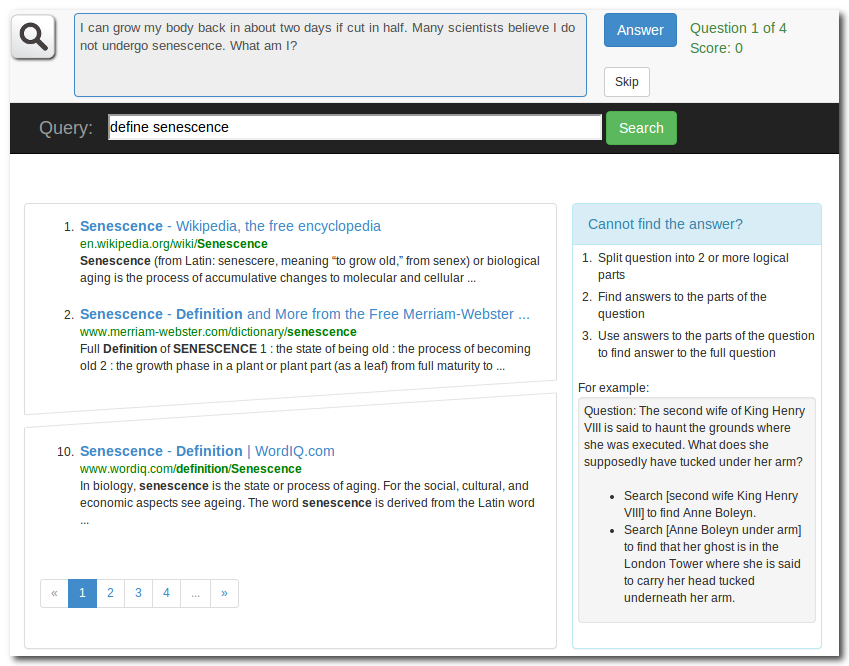
\includegraphics[width=\textwidth]{img/hints_ufindit}
\caption{The interface of the search game used in the study of the effect of strategic search hints on success in solving complex informational tasks.}
\label{figure:conversation:hints:ufindit}
\end{figure}

\begin{table}
\small
\centering
\begin{tabular}{r|p{4cm}|p{4cm}|p{4cm}}
& Question & Correct Answer & Specific hints \\
\hline
1 & I can grow body back in about two days if cut in half. Many scientists think I do not undergo senescence. What am I? & Senescence means ``biological aging''. Hydra is considered biologically immortal and regenerates fast. & \parbox[t]{4cm}{
1. Find what is senescence \\
2. Find who does not undergo senescence \\
3. Find who can also regenerate body and choose the one that satisfies both conditions} \\\hline
2 & Of the Romans "group of three" gods in the Archaic Triad, which one did not have a Greek counterpart? & Archaic Triad includes Jupiter, Mars, and Quirinus. Among those Quirinus did not have a Greek counterpart. &
\parbox[t]{4cm}{
1. Find the names of the gods from the Archaic triad\\
2. For each of the gods find a Greek counterpart
}\\ \hline
3 & As George surveyed the ``waterless place'', he unearthed some very important eggs of what animal? & "Gobi" in Mongolian means ``Waterless place''. The first whole dinosaur eggs were discovered there in 1923. & \parbox[t]{4cm}{
1. Find what is the ``waterless place'' mentioned in the question?\\
2. Search for important eggs discovery in this ``waterless place''}\\ \hline
4 & If you were in the basin of the Somme River at summers end in 1918, what language would you have had to speak to understand coded British communications? & Cherokee served as code talkers in the Second Battle of the Somme. & \parbox[t]{4cm}{
1. Find the name of the battle mentioned in the questions\\
2. Search for which coded communications language was used in this battle\\
} \\
\end{tabular}
\caption{Search tasks and specific search hints used for user study on the effectiveness of strategic hints for complex informational search tasks.}
\label{table:conversation:hints:tasks}
\end{table}

To estimate the effect of strategic search hints on user behavior we conducted a study in a form of a web search game similar to ``a Google a Day''\footnote{\href{url}{http://www.agoogleaday.com/}} and uFindIt \cite{Ageev:2011:FYG:2009916.2009965}.
Participants were hired using Amazon Mechanical Turk\footnote{\href{url}{http://www.mturk.com/}}.

The goal of the web search game was to find answers to several questions with the provided web search interface (Figure~\ref{figure:conversation:hints:ufindit}).
Players are instructed not to use any external tools.
The questions are given one by one and since tasks might be too difficult, a chance to skip a question was provided, although users were instructed that effort put into solving a question will be evaluated.
To answer a question each player needs to provide a link to a page containing the answer as well as its text.
The answer is automatically verified and a pop-up box notifies a player if the answer is incorrect (since the answer can be formulated differently, the presence of a keyword was checked).
A player can then continue searching or skip the question when she gives up.
A bonus payment was made to players who answer all questions correctly.
We used Bing Search API\footnote{\href{url}{https://www.microsoft.com/cognitive-services/en-us/bing-web-search-api}} as a back-end of the game search interface.
All search results and clicked documents were cached so users asking the same query or clicking the same page got the same results.
At the end of the game, a questionnaire was presented asking for feedback on user satisfaction with the game, prior experience, and other comments.

The tasks for the study were borrowed from the ``A Google a Day'' questions archive.
Such questions are factual, not ambiguous and usually hard to find the answer to a single query, which makes them interesting for user assistance research.
We filtered search results to exclude all pages that discuss solutions to ``A Google a Day'' puzzles.
To do this we removed pages that mention a major part of the search question or ``a google a day'' phrase.
To keep users focused throughout the whole game we limited the number of questions to 4.
The tasks are described in Table \ref{table:conversation:hints:tasks} and were presented to all participants in the same order to ensure comparable learning effects.

The questions have multiple parts and to solve them it is helpful to search for answers to parts of the questions and then combine them.
In one of the previous studies, we observed, that most of the users did not adopt the divide-and-conquer strategy, but kept trying to find the ``right'' query.
We decided to estimate the effect of strategic search hints, suggesting users to adopt the new strategy.

We built 2 sets of strategic hints: \textit{task specific} and \textit{generic}.
Task-specific hints described steps of one of the possible solutions to each question (Table \ref{table:conversation:hints:tasks}).
The second set contained a single hint, which was shown for all tasks. Generic hint described the divide-and-conquer strategy:\\

\hrule
\begin{enumerate}[noitemsep]
\item Split the question into 2 or more logical parts
\item Find answers to the parts of the question
\item Use answers to the parts of the question to find answer to the full question
\end{enumerate}

For example, the question: ``The second wife of King Henry VIII is said to haunt the grounds where she was executed. What does she supposedly have tucked under her arm?''
\begin{enumerate}[noitemsep]
\item Search [second wife King Henry VIII] to find Anne Boleyn.
\item Search [Anne Boleyn under arm] to find that her ghost is in the London Tower where she is said to carry her head tucked underneath her arm.
\end{enumerate}
\hrule
\vspace{5mm}

To control for the learning effect demonstrated in~\cite{Moraveji:2011:MIU:2009916.2009966}, each user was assigned to one of the three groups: (1) users who did not get any hints; (2) users who got task-specific hints; (3) users who got the generic hints.


\subsection{Results and Discussion}
\label{section:conversation:hints:results}

From 199 unique participants, who clicked the HIT on Amazon Mechanical Turk only 90 players finished the game.
We further examined all games manually and filtered out 9 submissions for one of the following reasons: lack of effort (\eg skipped several tasks after none or a single query) or usage of external resources (\eg the answer was obtained without submitting any queries or results explored did not contain the answer).
Furthermore, 10 players from the group which received hints indicated in the survey that they did not see them, so we filtered out those submissions and finally, we had 71 completed games (29 for no hints, 20 for task-specific hints and 22 for generic hints groups).

\textbf{Effects of Search Tips on Performance}.
In order to measure search success rate we looked at the number of questions answered correctly by different groups of users\footnote{Since users were allowed to skip a question we are counting the number of questions that were eventually solved correctly even if a player made some incorrect attempts.}.
Figure~\ref{figure:conversation:hints:task_success} shows that success rate is higher for users who saw task-specific hints compared to users who did not get such assistance.
Surprisingly, having the generic hint decreased the success rate, although users could easily ignore a hint they did not like.
A possible explanation is: generic hints were harder to follow and users who tried and failed became frustrated and did not restart their searches.

The plot of average time to answer a question on Figure~\ref{figure:conversation:hints:task_time} does not show an improvement for the task-specific hints group, except for the question 1.
Our task-specific hints represent a possible way to solve a problem and there is no guarantee, that it is the fastest one.
It is worth noting, that users from the generic search hint group had slightly higher variance in success time, which can probably be explained by the fact that some users were successful in finding the right way to follow the hint and some other users struggled with it much longer.
Another insight comes from the number of incorrect attempts users made.
Figure~\ref{figure:conversation:hints:incorrect} demonstrates the average number of incorrect answer attempts for all groups of users.
Although the variance is high, there is a tendency for users who saw task-specific hints to make fewer attempts than both other groups.
This is not in direct correspondence with time spent on the game.
It seems that the users who saw a clear strategy to solve the question were less likely to notice plausible, but incorrect solution.
Moreover, we analyzed texts of incorrect answers and can conclude that a big part of incorrect submission are due to users trying all possible options they found on the way, even if these options are clearly wrong.


\begin{figure}
\small
\centering
  \begin{subfigure}[t]{0.32\textwidth}
  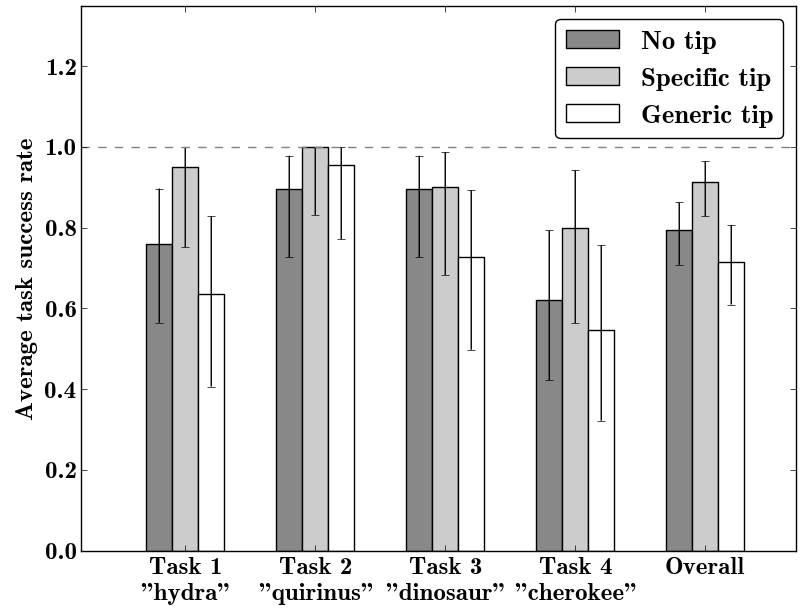
\includegraphics[width=\textwidth]{img/hints_success_per_task}
  \caption{Success rate per task for each group of participants}
  \label{figure:conversation:hints:task_success}
  \end{subfigure}
  \begin{subfigure}[t]{0.32\textwidth}
  \centering
  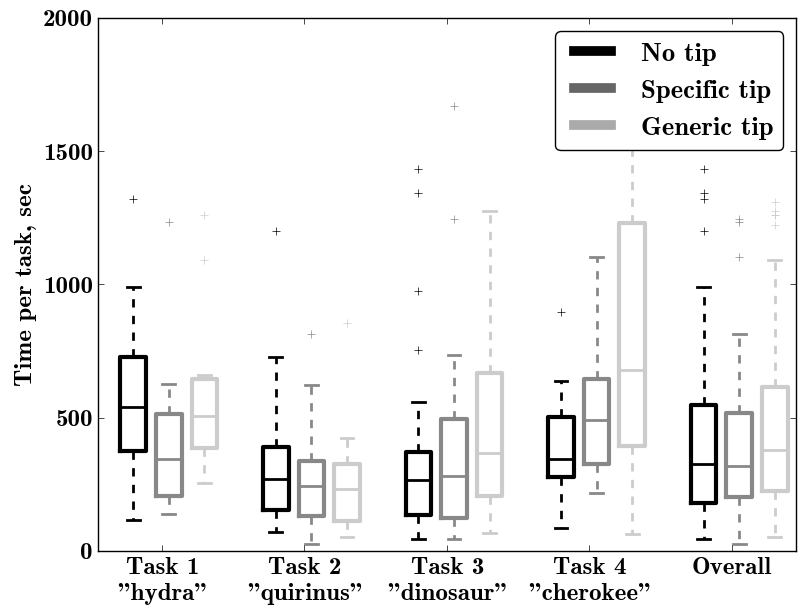
\includegraphics[width=\textwidth]{img/hints_time_per_task}
  \caption{Task completion time for each group of players}
  \label{figure:conversation:hints:task_time}
  \end{subfigure}
  \begin{subfigure}[t]{0.32\textwidth}
  \centering
  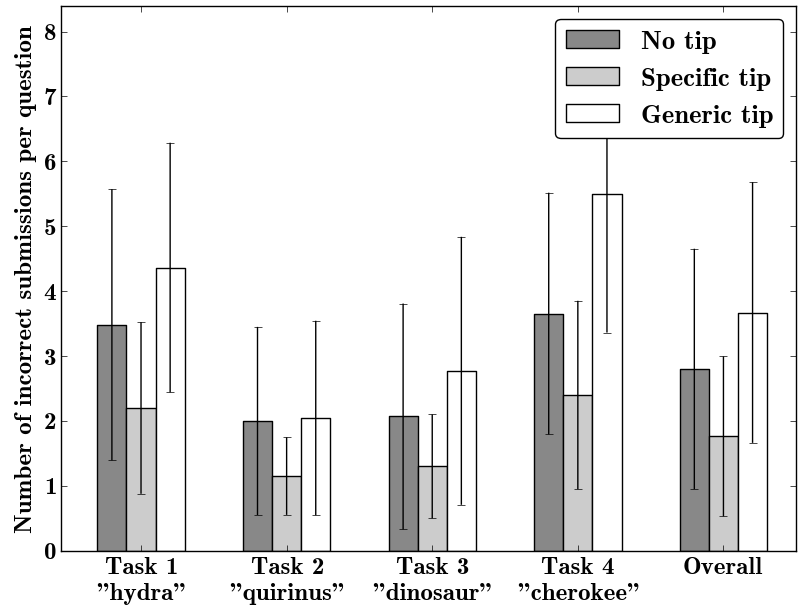
\includegraphics[width=\textwidth]{img/hints_incorrect}
  \caption{The number of incorrect submission attempts per question for all groups of users}
  \label{figure:conversation:hints:incorrect}
  \end{subfigure}
\caption{Results of the user study on the effectiveness of strategic search tips on search task success rate.}
\label{fig:conversation:hints:results}
\end{figure}

\begin{figure}[h]
\centering
\begin{subfigure}[t]{0.32\textwidth}
    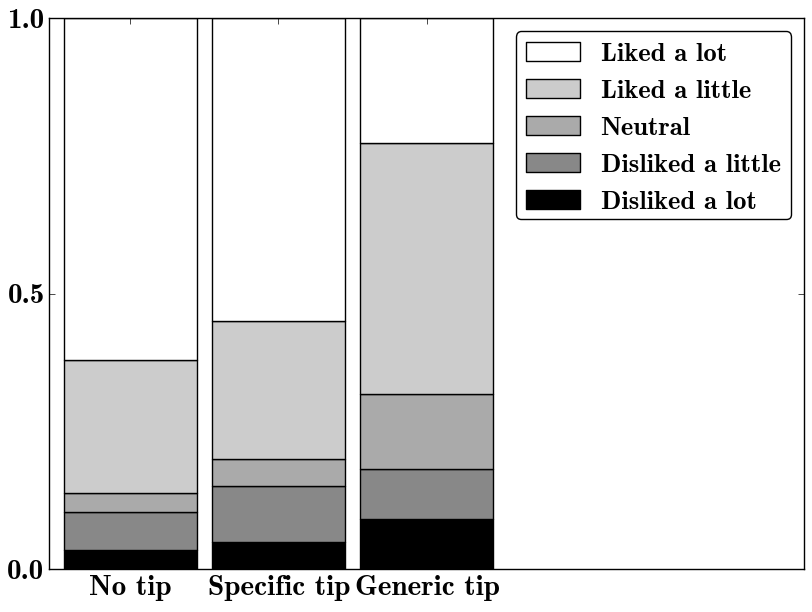
\includegraphics[width=\textwidth]{img/hints_liked}
    \caption{How did you like the game?}
    \label{figure:conversation:hints:survey:liked}
\end{subfigure}
\begin{subfigure}[t]{0.32\textwidth}
    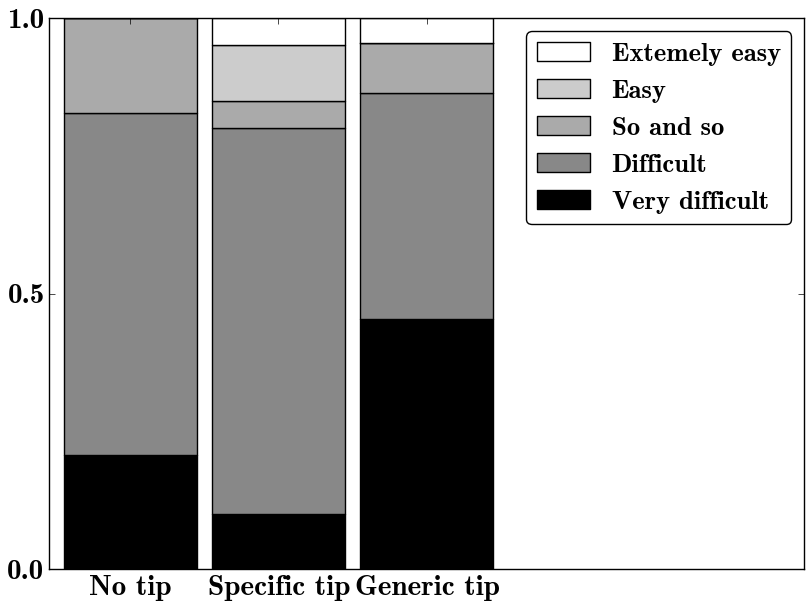
\includegraphics[width=\textwidth]{img/hints_difficult}
    \caption{How difficult was the game?}
    \label{figure:conversation:hints:survey:difficult}
\end{subfigure}
\begin{subfigure}[t]{0.32\textwidth}
    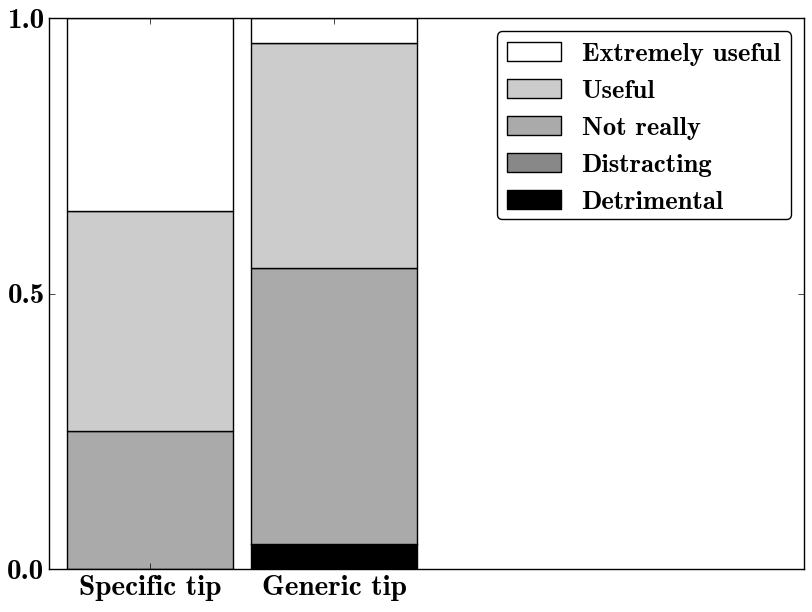
\includegraphics[width=\textwidth]{img/hints_useful}
    \caption{Were search hints useful to you?}
    \label{figure:conversation:hints:survey:useful}
\end{subfigure}
\caption{Proportions of replies to some of the survey question for each group of users.}
\label{figure:conversation:hints:survey}
\end{figure}

We also looked at other search behavior characteristics: number of queries submitted, the number of clicks made, the average length of the queries.
The variance in these characteristics was too high to make any speculations regarding their meaning.

\textbf{Effects of Search Tips on User Experience}.
Finally, we looked at the surveys filled out by each group of users.
Figure \ref{figure:conversation:hints:survey} presents proportions of different answers to three of the questions: ``How did you like the game?'', ``How difficult was the game?'' and ``Were search hints useful to you?''.
Surprisingly, user satisfaction with the game was lower for users who saw hints during the game and users who did not get any assistance enjoyed it more.
The replies to the question about game difficulty are in agreement with the success rate: users who saw task-specific hints rated difficulty lower than participants who struggled to find the correct answers.
The game was very difficult on average, however, some participants from the group who received task-specific hints surprisingly rated it as very easy, which suggests that our hints do help users.
This is supported by the answers to the last question on whether hints were helpful (Figure \ref{figure:conversation:hints:survey:useful}).

% To summarize, the results of the conducted user study suggest that specific search hints can be helpful, which is indicated by higher success rate, lower number of incorrect attempts and positive feedback at the end of study survey.
% In contrast, generic hints can have the negative effect on user experience, which is indicated by lower success rate, increased number of incorrect attempts and higher perceived tasks complexity according to the survey.

\subsubsection{Summary}
\label{section:conversation:hints:summary}

In this section, we studied the effect of strategic search hints on user behavior. 
The conducted user study in a form of a web search game demonstrated the potential of good hints in improving search success rate.
However, to be useful, they should be designed carefully.
Search hints that are too general can be detrimental to search success.
We also find that even searchers who are more effective using specific search hints, feel subjectively less satisfied and engaged than the control group, indicating that search assistance has to be specific and timely if it is to improve the searcher experience.

In addition to providing users with some hints on how to continue their search process, it is important for a QA system to improve question understanding skills.
Unfortunately, some questions contain certain ambiguity.
In conversational settings, a natural thing to do for such requests is to ask a clarification question, which is the focus of the next section of this dissertation.


% =================== Clarification questions : begin ======================

\section{Clarifications in Conversational Question Answering}
\label{section:conversation:clarq}

One key capability required to make conversational question answering effective is asking \textit{clarification questions} (\clarQ) proactively, when a user's intent is not clear, which could help the system provide more useful responses.
With this in mind, we make the first attempt to examine the clarification questions (\clarQ) that users ask on the Stack Exchange community question answering (CQA) platform.
We analyze Stack Exchange data in two domains
corresponding to about 300K questions and comments.
The contributions of this study are threefold:
\begin{itemize}[noitemsep]
\item To learn about user behavior associated with \clarQ and about their role in CQA communications. We find that \clarQ~are quite common on Stack Exchange, and therefore represent a good source of data for analysis.
\item To study the types of \clarQ~users ask in different situations. We classify clarification questions into several categories according to their target as well as syntactic patterns, which help define the space of \clarQ~for future research;
\item To make the first step towards automatic generation of \clarQ: 
we build a model to predict the subject of a popular type of clarification questions, which shows the potential of such approach for future research.
\end{itemize}

\subsection{Dataset Description}
\label{section:conversation:clarq:data}

\begin{figure}[t]
\centering
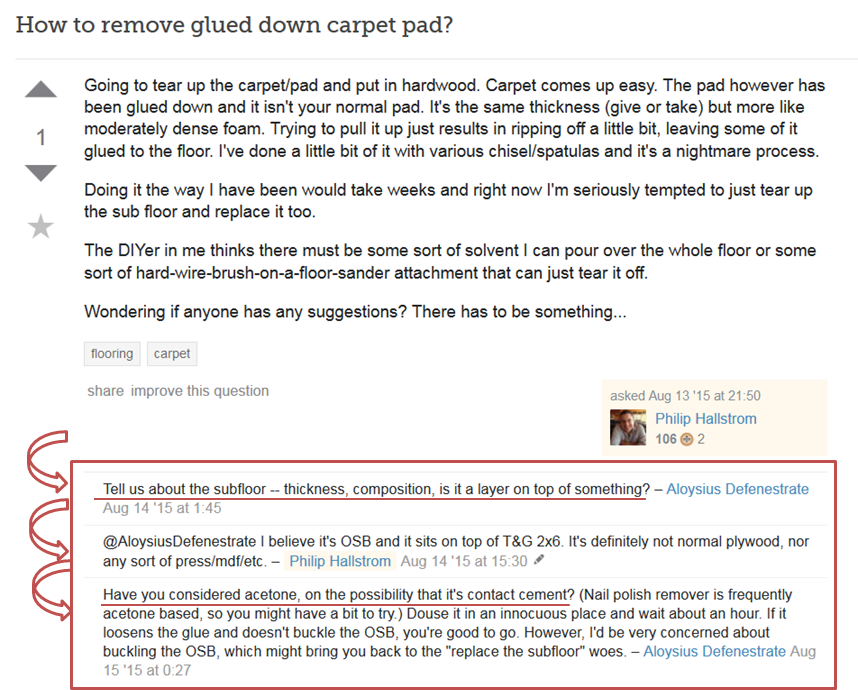
\includegraphics[width=0.95\textwidth]{img/diy}
\caption{Screenshot of a DIY question page from StachExchange CQA platform with threaded conversation in comments.}
\label{figure:conversation:clarq:diy}
\end{figure}

For our analysis we took two Stack Exchange sites -- Home improvements (DIY)\footnote{\href{url}{http://diy.stackexchange.com/}} and Arqade (GAMES)\footnote{\href{url}{http://gaming.stackexchange.com/}}.
These two domains are quite different -- the former is devoted to purely practical real-world problems, the latter -- to the virtual world of video games. Stack Exchange users can comment on the questions and answers;
sometimes it leads to multi-turn forum-like discussions (see Figure~\ref{figure:conversation:clarq:diy}).
The data dumps provided by Stack Exchange\footnote{\href{url}{https://archive.org/details/stackexchange}} cover a period of 5.5 years -- from July 2010 to January 2016. 

We define \clarQ~in a straightforward manner: sentences in comments to the initial questions ending with the question mark, provided by the users different from the asker of the initial question, four words and longer. This heuristic is not perfect, as clarification requests can be formulated as a declarative sentence, \eg \textit{Please provide details...} or question mark can be just missed. At the same time, these interrogative comments may be rhetorical questions, or not on the initial question's subject.
Nevertheless, manual inspection showed that this definition of \clarQ~is operational and allows extraction of \clarQ~ with precision acceptable for an exploratory study.

Basic statistics of the two datasets are reported in Table~\ref{table:conversation:clarq:data}.

\begin{table}[h]
\centering
\small
\begin{tabular}[t]{p{8cm}rr}
& \textit{DIY} & \textit{GAMES}\\
\hline
\# of questions & 20,702 & 62,511\\
\# of answers & 36,580 & 105,167\\
\# of accepted answers & 8,381 & 40,049 \\
\# of comments & 87,238 & 228,074\\
average question length in words & 130.8 & 86.5\\
average comment length in words & 33.8 & 25.8\\
\# of comments on questions & 37,296 & 96,247\\
\# of non-asker comments on questions & 27,873 & 72,495\\
\# of comments on questions with `?' & 11,040 & 21,448 \\
\clarQ~followed by asker's comments & 3,679 & 8,021 \\
\clarQ~followed by post editing & 4,270 & 9,038 \\
\clarQ~followed by post editing by asker & 1,631 & 3,772\\  
\end{tabular}
\caption{Statistics of the Stack Exchange datasets, used for the clarification questions study.}
\label{table:conversation:clarq:data}
\end{table}

\subsection{Results}
\label{section:conversation:clarq:results}

\subsubsection{User behavior}
\label{section:conversation:clarq:behavior}

As Table~\ref{table:conversation:clarq:data} shows, the presence of \clarQ~in CQA is substantial. Many characteristics such as questions/answers, accepted answers/all answers ratios are similar for both domains.
Questions and comments in DIY are longer then in GAMES, which is expected: DIY implies richer and more diverse contexts.
Askers are engaged in communication even after the initial question is posted: they comment on questions and edit them (however, questions are edited by community members more often).
Although there are more comments on questions in DIY, GAMES seem to be somewhat more conversational: askers respond to questions on questions more often.
Interestingly, thousands of initial questions are followed by clarifications, and in many cases, these are followed by the original question being edited, presumably in response to the clarification request. 

Unfortunately, we see that questions followed by \clarQ~do not differ much from questions without any comments in length -- a simple assumption that \clarQ~are targeted at short underspecified questions does not hold.
The hypothesis that questions asked by novice and less experienced community members (based on users' ratings) receive more \clarQ~is not supported either.
We also did not find any topical specificity of questions with \clarQ~based on tags. 

\begin{figure}
\centering
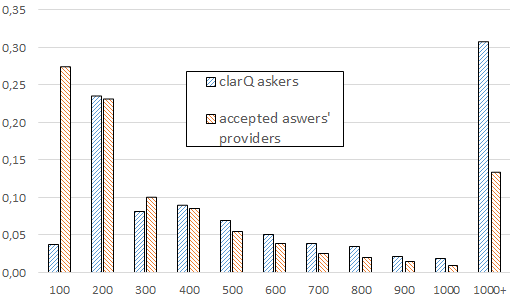
\includegraphics[width=.75\linewidth]{img/user_ratings.png}
\caption{Distribution of users' reputation scores in the groups of accepted answers' providers and commentators on questions (GAMES).}
\label{figure:conversation:clarq:users_scores}
\end{figure}

Figure~\ref{figure:conversation:clarq:users_scores} shows rating distribution of the GAMES users, who ask \clarQ~and those who provide accepted answers (i.e., the best answerers in the community).
We can observe that distribution for the former group is shifted towards higher scores (DIY exhibits a very similar distribution). 
However, the users who ask for clarifications provide answers for the initial questions very rarely. 
This observation suggests that \clarQ~in CQA are a form of `quality control measures' undertaken by most experienced users.


\subsubsection{Question types and patterns}
\label{section:conversation:clarq:types}

\begin{table}[h!]
\centering
\begin{tabular}[t]{lrl}
\textit{Category} & \textit{\%} & \textit{Example} \\
\hline
More Info & 28.6 & What OS are you using? \\
Check & 29.3 & Are you on a 64-bit system?\\
Reason & 8.5 & What is the reason you want a drip pan?\\
General & 10.2 & Can you add more details to this question?\\
Selection & 9.9 & Are you using latex or oil based Kilz?\\
Experience & 10.2 &  Have you tried to update video card drivers?\\
Not a \clarQ & 13.9 & Out of curiosity what elo are you? \\
\end{tabular}
\caption{The distribution of questions in StackExchange comments by type. Some comments contain several \clarQ of different types, so the sum is more the 100\%.}
\label{table:conversation:clarq:qtypes}
\end{table}

\begin{table}[h!]
	\centering
	\small
	\begin{tabular}[t]{p{4cm}rrp{5.5cm}}
		\textbf{Pattern} & \textbf{DIY} & \textbf{GAMES} & \textbf{Example} \\
		\hline
		\textit{have you tried}& 256 & 1,123 & Have you tried reinstalling the game yet?\\
		\textit{do you have}                 & 592 & 692 & Do you have enough disk space left?\\
		\textit{do you mean}                 & 248 & 552 & Do you mean a separate tub and shower? \\
		\textit{are you sure}                & 206 & 366 & Are you sure you have timber frame construction? \\
		\textit{what (is|are) the}             & 558 & 361 & What is the slope of the floor? \\
		\textit{what do you}                 & 103 & 284 & What do you mean by squeaking?\\
		\textit{(are|is) there any}            & 154 & 147 & Are there any airflow ducts in the room already?\\
		\textit{can you (post|provide)}     & 204 & 125 & can you post some pictures? \\
		\textit{how X (is|are)}                & 290 & 117 & how old is the water heater? \\
		\textit{is it a}                     & 186 & 112 & is it a constant 18-22 fps?\\
		\textit{what (kind|type) of}         & 344 & 106 & What kind of texture is on the wallpaper? \\
		\textit{why do you}                 &  73 & 101 & Why do you need to run it from the Flash drive?\\
		\textit{have you checked}             &  66 &  98 & Have you checked the frequency of the outlets? \\
		\textit{is it possible}             &  78 &  84 & Is it possible the tank is just over filling? \\
		\textit{do you know}                 & 120 &  64 & Do you know the manufacturer of the fixture?\\
	\end{tabular}
	\caption{Question patterns in comments (sorted by frequency in GAMES) from StackExchange dataset.}
	\label{table:conversation:clarq:patterns}
\end{table}


In order to investigate \clarQ~breakdown by type, we sampled 294 comments on questions from both domains, and two authors performed manual annotation analogously to~\cite{kato2013}, see results in Table~\ref{table:conversation:clarq:qtypes}.
Comments that are not aimed at clarifying the main question contain rhetorical or humorous questions,
questions to previous comments, citations of other questions on the platform, etc. Interestingly, the breakdown of \clarQ~by type is roughly the same as in~\cite{kato2013}.

Further, upon examining the sample we identified a list of common three-word question starting patterns, and calculated their frequency in the whole dataset, see Table \ref{table:conversation:clarq:patterns}. 
As can be seen from the Table~\ref{table:conversation:clarq:patterns}, some patterns are quite indicative for the clarification type (\eg \textit{what kind of} corresponds to \textit{More info} category, whereas \textit{have you tried} -- to \textit{Experience}).
This observation suggests that recognition of clarification question type is a feasible task.


\subsubsection{Clarification subject prediction}
\label{section:conversation:clarq:subj-prediction}

As we have shown, there are many different kinds of questions that users ask in comments.
Many of them address a certain ambiguity present in questions, \eg \textit{what kind of} questions inquire about a subtype of a mentioned object.
These questions are quite common (Table~\ref{table:conversation:clarq:patterns}) and have a simple structure, which makes them a quite appealing target for automatic question generation.
The first step for such question generation is to predict the object to ask about.
We collected questions, which received at least one \textit{what (kind|type) of} \clarQ~in DIY. 
From these comments and questions, we extracted noun phrases using Stanford CoreNLP parser~\cite{manning-EtAl:2014:P14-5}, and kept only those questions that have a common pair of noun phrases in the question and comment.
We formulated the task as the noun phrase ranking problem, where the noun phrase from the comment should be placed higher on the list than other noun phrases from the question.
Each candidate phrase was represented by the following set of features:
\begin{itemize}[noitemsep]
\item \textbf{prior}: number of times the noun phrase was used in comments (separate from the training and test sets)
\item \textbf{topicality}: number of occurrences of the phrase in the current question (in title and body together)
\item \textbf{position}: position of the first occurrence of the noun phrase relative to the beginning of the question
\item \textbf{entropy}: collection-based statistic, computed using all noun phrases that contain the given noun phrase, which estimates the number of different modifications of the current noun phrase object
\item \textbf{length}: number of words in the noun phrase
\end{itemize}

To train the ranking model we used a random forest algorithm implemented in the RankLib library\footnote{\href{url}{https://sourceforge.net/p/lemur/wiki/RankLib}}.
We optimized DCG@10 and Table~\ref{table:conversation:clarq:np_rank_performance} summarizes the performance metrics on 10-fold cross validation.
As we can see, even with a limited set of features our model was able to place the true subject of a clarification question above other candidates in 35\% of the cases.
To study the contributions of different feature groups we conducted a series of experiments to train the model with each group individually.
The results in Table~\ref{table:conversation:clarq:np_rank_performance} suggest, that the number of occurrences of a phrase and the position of the first occurrence are strong features, and confirms our intuition that \clarQ~are usually asked about the main topic of the question.
However, some noun phrases are more ambiguous in general, therefore the prior feature also contributed significantly to the quality of the model.

\begin{table}[h]
\centering
\begin{tabular}[t]{lrrrr}
\textit{Model} & \textit{P@1} & \textit{MAP} & \textit{RR@10} & \textit{ERR@10} \\
\hline
random & 0.077 & 0.215 & 0.231 & 0.015 \\
+ entropy & 0.143 & 0.334 & 0.350 & 0.024 \\
+ length & 0.148 & 0.337 & 0.345 & 0.024 \\
+ position & 0.165 & 0.335 & 0.357 & 0.024 \\
+ prior & 0.214 & 0.402 & 0.427 & 0.030 \\
+ topicality & 0.319 & 0.426 & 0.473 & 0.032 \\
all features & 0.350 & 0.508 & 0.549 & 0.038 \\
% random & 0.0769 & 0.2151 & 0.2305 & 0.0146 \\
% + entropy & 0.1425 & 0.3336 & 0.354 & 0.0244 \\
% + length & 0.1481 & 0.337 & 0.3498 & 0.024 \\
% + position & 0.1652 & 0.3346 & 0.3568 & 0.0237 \\
% + prior & 0.2137 & 0.4018 & 0.4266 & 0.03 \\
% + topicality & 0.3191 & 0.4255 & 0.4731 & 0.0315 \\
% all features & 0.3504 & 0.5078 & 0.5491 & 0.0381 \\
\end{tabular}
\caption{Performance metrics (P@1 -- precision at~1, MAP -- mean average precision, RR@10 -- reciprocal rank at 10, ERR@10 -- expected reciprocal rank) of the ranking model for ``ambiguous'' noun phrase selection problem.}
\label{table:conversation:clarq:np_rank_performance}
\end{table}

Overall, our experiment showed promising results for predicting the subject for a certain type of \clarQ.
As a next step, our model can be combined with an ambiguity detection classifier, which would trigger clarification as a response from a conversational search agent.

\subsection{Discussion}
\label{section:conversation:clarq:Discussion}

As a step towards general-purpose interactive QA system, we analyzed clarification questions asked by CQA users.
In particular, we examined user interactions related to \clarQ, as well as the role and place of these questions in  CQA.
We analyzed a large sample of \clarQ according to their type and identified most common syntactic patterns in a large collection of \clarQ.
Finally, we conducted an experiment aimed at automatically detecting the subject of clarification question of a particular type.

Based on our analyses, we can conclude that \clarQ~are common in CQA archives, and introduce a valuable resource for user behavior studies and QA research.
Clarification questions asked by community members are an important component in maintaining the quality of user-generated content in CQA.
Furthermore, we see that clarification questions are quite diverse in topic and style, are highly dependent on context and individual characteristics of the users.
However, there are several types of questions and syntactic patterns that are common within each domain.
As a first step towards automatically generating clarification questions, we show promising results on identifying the subject of \clarQ~based on a small set of shallow features.
Our findings suggest that CQA data may be useful for research in the field of interactive QA.

% There is still a long way to go towards automatic generation of clarification questions.
% This capability would require identification of user questions which are indeed ambiguous, choosing an aspect and type of clarification, and generate the text. 
% These steps imply naturally an analysis of answer candidates, which was not addressed in the current work. 
% A significant portion of \clarQ deals with properties, attributes, relations and types of the objects mentioned in the initial question.
% This suggests that domain-specific knowledge-based approach to \clarQ~generation can be promising. 
% These two tasks -- the use of candidate answers and knowledge bases -- define the directions for future research in the area of clarification questions generation for interactive QA.


% =================== Clarification questions : end ======================

\section{Summary}
\label{section:conversation:summary}

This Chapter described the research I have done on conversational question answering, which gives a system opportunities to exploit a rich set of possible interactions with its users.
First, I described the design and implications of the user study we conducted to investigate the current state in conversational search, and looked into what users expect from a dialog agent compared to a human interlocutor, and what is missing from an existing state-of-the-art commercial system.
We learned, that users do not have any prejudice towards automatic question answering agents, and for some people they are actually preferable, avoiding certain social norm issues.
We identified some directions for future research in order to move existing systems towards user expectations, by providing a diverse set of opinions as well as information sources, improving context maintenance techniques, and learning from user feedback.
As the first steps in these directions, I discussed search hints and clarification questions, which can be provided by the system to either help users structure their search process or clarify some of the ambiguities.
The results of the conducted research showed that hints tailored to a specific search problem can effectively guide the user through the search process.
However, generic hints might actually take away the feeling of control from the user and lower both satisfaction and success rate.
To study the phenomenon of clarification questions, we analyzed the data from one of the community question answering platforms and identified different types of clarifications, \eg ``what type of ...'' questions, that aim at requesting information on a particular type of an object mentioned in the question.
The model we built to predict the subject of such questions showed a reasonable performance, and demonstrate the potential of this approach for automatic clarification generation.

Together, the research described in this chapter provides desiderata for future developments in conversational search and question answering and shows promising first steps in some of these directions.		\clearpage
\chapter{Conclusions}
\label{chapter:conclusion}

This chapter concludes the dissertation by providing the summary of the findings, limitations, potential future directions, and the main contributions of my work.

\section{Summary of the Results}
\label{section:conclusion:summary}

In the era of information overload, we have to rely on intelligent systems to help us organize and search the knowledge about the world.
The research described in this dissertation aims to improve the technology behind question answering systems, which can sift through the constantly growing piles of information and give the user the needed response.
In the next sections, I will describe the main results of my research, and how it helps to get closer to the above-mentioned goal.

\subsection{Combining KB and Text Data for Factoid Question Answering}
\label{section:conclusion:summary:factoid}

When we type a question like ``\textit{What is the capital of Peru?}'' into a favorite search engine, we can expect to see a direct answer shown on top of search results.
However, for the majority of more complex tail questions users still have to browse through retrieved web documents and search for the answer themselves.
My Ph.D. research targets the problem of improving both precision and recall of factoid question answering by combining available data sources.
Chapter~\ref{chapter:factoid} described 3 different approaches to this problem.

Relation extraction became a common tool for transforming knowledge from one format to another, \eg from natural language text into structured knowledge base triples.
Existing approaches target some particular subsets of data, \eg facts expressed in statements, such as ``\textit{The capital of Peru is Lima}''.
The proposed model for relation extraction from community generated question-answer pairs (Section~\ref{section:factoid:cqarelextract}) provides an extension of existing techniques to a new domain and helps to extract additional factual triples, therefore increasing the coverage of knowledge bases.
Our experiments on Yahoo!~Answers and WikiAnswers datasets suggest, that by adding the proposed model, which focuses on entity pairs mentioned in the question and answer texts, we can extract $\approx 30\%$ more triples, compared to existing sentence-based techniques.
Extracted triples can be further injected into a knowledge base, \eg using approaches like Google Knowledge Vault~\cite{Dong:2014:KVW:2623330.2623623}, eventually leading to a better coverage, and more answered user questions.

Besides increasing the coverage of underlying data, the dissertation proposes a set of techniques to improve the performance of the core question answering pipeline.
\textit{Text2KB} model, described in Section~\ref{section:factoid:text2kb}, brings the power of text-based question answering to KBQA to improve question interpretation, candidate generation and ranking.
By identifying mentions of knowledge base concepts in text documents it is possible to use text matching techniques to understand the question topic, relate question terms to KB predicates and better rank the generated answer candidates.
The experiments conducted on the WebQuestions benchmark dataset demonstrated, that the proposed techniques can improve the performance of a state-of-the-art KBQA system by $\approx 8\%$.

Finally, the dissertation proposes the \textit{EviNets} neural network framework, which can aggregate answers supporting evidence from different sources, including text and knowledge base data.
By embedding text and KB triples into the same space, the model can estimate the relevance of each statement to the question, and score candidate answers based on their all available evidence.
The experiments performed on TREC QA, WikiMovies and new developed Yahoo!~Answers datasets confirm these expectations and demonstrate that the model indeed can combine KB and text data in a unified framework, improving the performance over existing baseline approaches.

Combined, the techniques proposed in the dissertation allow us to achieve both higher precision and recall in factoid question answering.

\subsection{Ranking Answer Passages for Non-factoid Question Answering}
\label{section:conclusion:summary:non-factoid}

The challenges in non-factoid question answering are due to a diverse nature and types of these questions and answers.
During my Ph.D. studies, I developed a system, that combines vertical search in CQA archives and general web search to retrieve similar question-answer pairs and text passages from relevant documents.
The system achieves state-of-the-art performance in TREC LiveQA 2015 and 2016 shared tasks and can be used as a baseline for future experiments.
According to the results of TREC LiveQA 2016, for more than half of the questions the system was able to return a relevant response, and for $\approx 20\%$ of the questions it gave a perfect answer.

The crowdsourcing module, integrated into \textit{EmoryCRQA} system for obtaining additional answer candidates, and ranking of existing ones, allowed us to significantly boost the performance of the fully automatic QA system.
This hybrid system achieved the highest score among participants of the TREC LiveQA 2016 shared task, with the average answer score of 1.260 on the 1-4 Likert scale.
This score is only within $\approx 20\%$ of this of community-generated response, which was obtained a week after.
The experiment demonstrates, that it is possible to use a crowd of non-expert workers to obtain additional feedback and relevance judgments in real-time, and these signals can significantly improve the performance of an automatic QA system.
Even without special domain expertise random workers were able to contribute additional and judge the relevance of existing answer candidates, and both of these contributions have an equally positive impact on the overall performance.
With crowdsourcing, our system was able to generate a reasonable response to more than $60\%$ of the questions, compared to only $50\%$ for the fully automatic setup.
The crowdsourcing expenses can be reduced by limiting the number of workers per single task and selectively requesting feedback for more complex questions only.
These findings can be useful for building hybrid question answering systems, that would rely on human feedback to improve performance on difficult tasks.


\subsection{Question Answering in Conversational Setting}
\label{section:conclusion:summary:conversation}

While gaining some popularity, personal assistants like Amazon Alexa, Google Home, Microsoft Cortana and Apple Siri, are still mostly used for simple routine tasks, like playing music and checking the news and weather.
In Section~\ref{section:conversation:user-study} we described a user study, designed to learn what is missing from commercial products to be the major tool for informational tasks.
The findings of the study suggest, that users still often prefer search engines because they can offer a variety of data with sources, and give more control over what information a user consumes.
The abilities of existing personal assistants often do not allow natural ways of forming questions, like a person would do in a conversation with an expert.
For example, the commercial chatbot we tested could not properly maintain the context of the conversation, \eg resolve pronouns to the previously mentioned topics.
However, the participants of the user study expressed their interest in such systems, as they allow to shortcut some social rules and get straight into the information finding while providing concise responses.
These findings highlight directions for future research in conversational question answering.

In Sections~\ref{section:conversation:hints} and~\ref{section:conversation:clarq} the dissertation describes some of the first steps in the discovered directions.
For complex search tasks, it is quite important to learn to formulate good search queries, as confirmed by the popularity of query suggestion and other assistance techniques.
The user study we conducted tested how users would react and benefit from strategic search hints, which propose a way to split the original difficult search task into simpler intermediate goals.
When dealing with a complex multi-step question, a conversational system can report a failure to answer and use such hints to suggest next steps to resolve the issue to the user.
The results of the user study reveal, that such hints can be helpful if designed carefully.
However, such assistance takes away some satisfaction from the search process.

As some of the user questions are ambiguous, a conversational system should be able to ask clarifications.
By analyzing the data from StackExchange CQA platform we can conclude that clarifications are a common phenomenon in human information seeking dialogs.
Clarification questions vary by type and form, however, there are some frequent patterns, which can be used to automatically generate questions to resolve ambiguities about objects, mentioned in the question.
As a proof of concept, we built a model to predict objects of ``what kind of ...'' clarification questions.
The performance of this model proves the feasibility of such an approach for template-based clarification question generation.

\section{Limitations and Future Work}
\label{section:conclusion:future_work}

In this Section, I summarize some of the limitations of the describe approaches and results and propose directions for future research.

Community question answering websites became quite popular and accumulate millions of question and answers, that people are interested in.
Therefore, they are quite valuable as a knowledge source, which can be reused to answer future user questions.
Relation extraction approach, proposed in this dissertation, was designed to extract subject-predicate-object triples for a schema-based knowledge base, such as Freebase.
However, many of the user questions do not align well with an existing schema, which restricts the scope of the model.
To resolve this issue, the future work can include developing methods for open information extraction from question-answer pairs, and extracting new predicates for schema-based KB, \eg using approaches similar to~\cite{Gupta:2014:BOS:2732286.2732288}.

Text2KB model, proposed in this dissertation to improve knowledge base question answering by employing techniques from text-based question answering, demonstrated its effectiveness on the WebQuestions benchmark.
However, for candidate generation, it mainly relies on KB data, which, as we saw, often does not contain predicates or entities, that user is asking about.
The EviNets model was designed to resolve this issue by considering both KB and Text data equally, and score answer candidates based on the support extracted from the various pieces of evidence.
One of the limitations of EviNets is that a set of candidate answers and pieces of evidence are ``pre-computed'' and cannot be extended during the model evaluation.
A possible future direction is to extend the evidence pool at run-time and turn to the reinforcement learning techniques for training.
In this case, the problem could be cast as a graph search problem, where entity nodes are connected with either retrieved textual evidence, or KB predicates, or both.
Another limitation of EviNets is the focus on single entities, whereas answers to many real user questions might be lists, and contain attributes, such as dates, numbers, \etc
To cover these answer types we can look into existing research on answer extraction, such as the research conducted on the SQuAD dataset~\cite{rajpurkar2016squad}, where the goal is to extract an answer span from a passage of a Wikipedia article.
It is possible to adopt these techniques to generate candidates, and aggregate all the evidence for each of them using EviNets.

Most of the existing approaches to non-factoid question answering, including the system presented in this dissertation, also rely on ranking existing passages, extracted from somewhere on the web.
The limitation of such an approach is that it does not give a big picture of all the relevant information available out there, suggests an answer, which might not be trustworthy, and/or gives a one-sided opinion on the issue.
In the user study on conversational search, we found out that users care about the source of the information, and want to get a diverse set of opinion.
While some approaches for answer summarization have recently been proposed~\cite{song2017summarizing,tomasoni2010metadata,wang2016query}, the problem is still far from being solved and might require a generative summarization approach~\cite{gambhir2017recent,mitra2016distillation}.

The effectiveness of the crowdsourcing approach for real-time question answering, proposed in this dissertation, is shadowed by its cost.
EmoryCRQA involved crowdsourcing for every question, which requires maintaining a pool of workers constantly ready to assist.
While we presented an analysis to reduce the costs by using less human resources, the future research should look into how to optimally plan question answering and optimize the cost/quality trade-off.
A question answering system or personal assistant should turn to crowdsourcing selectively when it was not able to come up with a good response itself.
On the other hand, some of the user questions might not be urgent, which allows the system to engage slower, but more reliable community of experts on one of the domain-specific CQA websites.
I believe, that future personal assistants should be able to plan and route questions more effectively given the type of question, their time and cost requirements.

The research on chatbots and conversational question answering are at its beginning, and the findings of the presented user study sheds some light into the areas we all should focus on, \eg methods for maintaining context in a conversation, generating clarification questions, taking positive and negative feedback \etc
The limitation of our user study is that we did not consider the voice interface, which adds certain specifics to how a system should present its results~\cite{trippas2015results}.
Some of the participants of our user study also raised an interesting point, that web search offers a possibility to browse related information and stumble upon something unexpected.
For example, when doing a research into the economics behind hydropower, a typical web page will cover multiple related topics, which would require a user to ask multiple questions, and actually assumes you are aware of all these aspects beforehand.
Research into ways to discover and present such related information in a conversational search setting might change the user experience significantly, and bring serendipity to the chat and voice interfaces.


\section{Contributions and Potential Impact}
\label{section:conclusion:contributions}

My Ph.D. dissertation covers a spectrum of aspects related to answering user information needs.
The key element of the proposed techniques and methods is an idea of combining and aggregating information from various unstructured (text), semi-structured (question-answer pairs) and structured (knowledge base) data sources.
This allowed us to exploit advantages of one source to overcome the disadvantages of the other sources, and improve precision and recall of automatic non-factoid question answering.
I believe, that this idea of information aggregation will be a key component of future intelligent systems, which should be able to reason with all the available knowledge, rather than simply returning the best matching item.
The models I developed in my dissertation demonstrate the potential of this approach and provide some insights for future research in this direction.

In addition to improving the core question answering techniques, it is important to optimize the channel, used to communicate with users.
The dialog is a natural activity, that human perform on a daily basis, and proliferation of mobile personal assistants suggest, that conversations might be the next step for information seeking scenarios.
In my dissertation, I presented the results of the user study, which provide the insights on how people use conversations for information seeking tasks, what are the expectations from the personal assistants, and what is currently missing from the commercial systems.
I believe, that this user study is an important step for future research in conversational search, and the suggested directions will help us develop next generations of the systems, that will gain wider adoption and will be quite helpful in everyday life.
Additionally, we explored two particular dialog scenarios for complex informational tasks.
Search hints and clarification questions are two possible response types a question answering system can return for complex or ambiguous questions, instead of returning empty or irrelevant answers.
Both of these types of interactions integrate nicely into a dialog scenario and enrich the arsenal of tools a conversational system possess in order to help user satisfy her goals.

Overall, this dissertation describes methods and techniques for improving the performance of question answering systems by combining various user-generated content, including those created on the fly with crowdsourcing.
These techniques can be integrated into a conversational personal assistant, and the dissertation gives some insights on the expectations and desiderata from such a system, obtained via user studies.
The contributions of this dissertation should help develop the next generation of the systems, that will help serve more than 1.2 trillion information searches per year\footnote{\href{url}{http://www.internetlivestats.com/google-search-statistics/}} for more than 3.5 billion internet users.

%that will help all of us orient in yearly zettabytes\footnote{1 ZB = $1000^7$bytes = $10^{21}$bytes = 1,000,000,000,000,000,000,000 bytes} of data traffic.

		\clearpage
% \myappendix

Here comes the appendix.


\clearpage
\addcontentsline{toc}{chapter}{Bibliography}

%%%%%%%%%%%%%%%%%%%%%%%%%%%%%%%%%%%%%%%
% The bibliography
%%%%%%%%%%%%%%%%%%%%%%%%%%%%%%%%%%%%%%%
\bibliography{thesis}
\bibliographystyle{plain}

\end{document}
